\documentclass[
    % twosupervisors, % uncomment if two supervisors
    11pt,
    a4paper
    ]{mphilthesis}
% options other than twosupervisors are passed to \documentclass[titlepage]{article}
% packages already loaded: amsmath, graphicx, hyperref, natbib, amsthm, thmtools, thm-restate, appendix 

\usepackage{blindtext}
\usepackage{amsmath}
\usepackage{bbm}
\usepackage{bm}
\usepackage{chngpage}
\usepackage{adjustbox}
\usepackage{rotating}
\usepackage{afterpage}




\DeclareMathOperator{\argmax}{argmax}
\usepackage{amssymb}
\usepackage[mathscr]{eucal}

% add here more packages or macros if needed

\author{Gabriela Mara Miyazato Szini}
\title{Correcting for Sample Selection Bias in Dyadic Regressions \\ \large An Application to Gravity Models}
\degree{Master of Philosophy in Economics (research)}
\degreedate{Amsterdam, August 2020}
\college{Tinbergen Institute}
\university{University of Amsterdam}
\supervisor{Prof. Dr. Frank Kleibergen}
\affiliation{University of Amsterdam}
\supervisorB{Dr. B}
\affiliationB{University of B}
\logourl{ti_logoblok.jpg}

\begin{document}
\maketitle
\afterpage{%
\thispagestyle{empty}
\section*{Acknowledgements}

I am extremely greatful to my supervisor Professor Frank Kleibergen. Not only he helped me a lot in shaping my agenda for this thesis, while still allowing me to follow my interests, but he was also extremely patient with me throughout this process. I can definitely say that I learned a lot from him.

I would like to thank my parents, Rosane and Alexander Szini, and my grandparents, Marilene and Missao Miyazato, for the unconditional support they have always provided me since I was a child. Without their support I would not be able to be here at the Tinbergen Institute today. I am also greatful for Roberto Padovani and Professor Vladimir Ponczek for having incentivized me to pursue an academic career since my bachelor days.

I truly appreciate all the comments about this study and my earlier drafts made by Anna Buijsman, Timo Schenk, Mariia Artemova, Julius Il\u{c}iukas, Carlos Lopes and Paloma Assun\c{c}\~{a}o. Finally, I would like to thank all my colleagues at TI that made this journey more fun.

\vspace{20mm}
\begin{flushright}
    \textit{To the memory of Istv\'{a}n Szini}
\end{flushright}
}
\clearpage




\begin{abstract}
We present methods to correct for sample selection bias in the estimation of dyadic regressions. Dyadic datasets can be seen as a pseudo panel data, where both dimensions tend to infinity as the number of individuals grows. We show that including fixed effects for both individuals forming a dyad leads to asymptotically biased estimates of the structural parameters in the first stage of the \cite{heckman1979sample} two step method. This is a consequence of the incidental parameter problem. We reconcile and modify existing approaches to similar problems in standard panel data models to this framework. Our Monte Carlo simulation exercise corroborates to the theoretical predictions that the standard Heckman approach yields biased estimates, while the proposed methods reduce such biases. We apply the proposed estimators to the gravity model for international trade flows. The suggested methods deliver different estimates for the coefficients of trade barriers.
\end{abstract}
\tableofcontents

\newpage 
\section{Introduction} \label{introduction}
\cite{tinbergen1962shaping} established gravity equations, which have been widely used for estimating models of international trade, migration, equity and FDI flows. For instance, in the literature of international trade flows, it is used to infer the effects of institutions such as customs unions, exchange rate mechanisms, ethnic ties, linguistic identity and international boarders on trade flows. 

Even decades after its first appearance in trade models, there is still a substantial lack of understanding on features of its estimation, and econometric methods that considers some potential issues only emerged recently in the literature. The aim of this paper is to provide an ample and deep discussion about different estimation issues in gravity models focusing on its dyadic structure, highlighting and describing in detail proposed estimators that take it into account. 

A great deal of applications rely on the specification of the gravity model proposed by \cite{helpman2008estimating}, due to its tractability and the fact that it demonstrates explicitly how the sample selection problem plays a role in the macroeconomic model. Up to this seminal paper, most studies only considered observations with positive trade flows when estimating such model without imposing any special treatment on it. However, the authors point out that one should account for the self-selection of firms into export markets and their impact on trade volumes. In other words, one should account for sample selection in the estimation. To do so, the authors first relax some assumptions in the theoretical foundation of the gravity model proposed by \cite{anderson2003gravity}, then they propose a parametric estimation of a linear model controlling for the sample selection through the inverse Mills-Ratio approach (\cite{heckman1979sample}). 

However, we show that this methodology suffers from the incidental parameter problem, \cite{neyman1948consistent}. This well-known problem relates to the fact that, as demonstrated by \cite{fernandez2016individual}, the fixed effects estimates in nonlinear models are asymptotically biased, even when both dimensions of a panel dataset tend to infinity. The model proposed by \cite{helpman2008estimating} undergoes such issue, once it accounts for fixed effects for both importer and exporter, which are known in the literature as the multilateral resistance terms.

In order to analyze such problems, and discuss possible solutions to it, we further simplify the estimated equations by \cite{helpman2008estimating}. This simplification highlights the fact that such a framework is applicable to any dyadic data. As defined by \cite{graham2020dyadic}, dyadic data reflects situations where the outcome of interest is determined by pairwise interactions between units. More specifically, the first stage of the estimation - that relies on estimating the probabilities that two units (nodes) interact with each other (that countries trade in the trade application) - delineates a specification for network formation. One particularity of dyadic settings is that as the number of individuals increase, both dimensions of the pseudo panel increase.

The introduction of two-way fixed effects requires that in the first stage of the approach, a more involved estimator needs to be employed to difference out such fixed effects, delivering asymptotically unbiased and consistent estimates for the structural parameters. A clever approach is proposed by \cite{charbonneau2017multiple} and employed in this study. This approach is based on a conditional likelihood estimator.

Once such estimates are obtained, the standard Heckman approach for correcting for sample selection in the observation equation requires that (i) estimates of the fixed effects itself in the first stage (selection equation) are provided such that the predicted probabilities are obtained; and (ii) a functional form for the inverse Mills-ratio is provided, which generally follows from both errors being normally distributed. The \cite{charbonneau2017multiple} estimation results in additional problems related to both items: it does not deliver estimates for the fixed effects itself, and it relies on the assumption that the errors of the selection equation are logistically distributed.

We propose two different approaches to tackle such obstacles. The first is to retrive the estimates of the fixed effects through the traditional unconstrained MLE, by setting the structural parameters to be equal to the estimates provided by \cite{charbonneau2017multiple}. This method is denoted by the hybrid approach by \cite{martin2018bls}. Once the fixed effects estimates are obtained, one can then calculate the predicted probabilities. Moreover, a transformation of the variables proposed by \cite{lee1983generalized} guarantees that the traditional two-step approach given by \cite{heckman1979sample} can be employed, even if the error term of the selection equation is logistically distributed.

A second approach is developed by \cite{kyriazidou1997estimation}. It relies on a weighted least squares estimator based on the idea of differencing out the sample selection effects in the observation equation (the second stage equation of \cite{heckman1979sample}), and, in the trade application, in the estimates for the volumes traded amongst countries. The advantage of this method is that, as we will demonstrate later, it does not require estimates of the fixed effects in the first stage equation. While the original framework in \cite{kyriazidou1997estimation} is a standard panel data model, where equations are differenced over the time dimension, we propose modifications of this approach to accomodate dyadic interactions, where equations are differenced over combinations of dyads. Such modification delivers an approach that can be employed even when the exogenous variables of the observation equation are invariant over time, varying only over dyads.

Even though the proposed approaches already exist in the literature separately (apart from our modification to the estimator proposed by \cite{kyriazidou1997estimation}), this study adds to the literature in that it combines those separate methods to account for sample selection in dyadic structures. Up to our knowledge, although the literature for sample selection corrections is abundant for standard panel data models, it is insufficient for dyadic datasets, and consequently for cases related to network formation.

The structure of this paper is as follows: Section \ref{gravity_model} presents the baseline gravity model by \cite{helpman2008estimating}, Section \ref{estimating_helpman} presents the estimation strategy employed by the authors, Section \ref{model} delineates our simplification of the model, highlighting its dyadic structure and its aspects related to network formation, Section \ref{section_heckman} provides the standard two-stage Heckman approach for this model, Section \ref{section_incidental_parameters} refers to a more formalized discussion of the incidental parameters problem, Section \ref{section_charbonneau} discusses the approach by \cite{charbonneau2017multiple}, Section \ref{first_approach} shows our first proposed approach to correct for sample selectivity in the observation equation, Section \ref{sample_selection_alternative} shows the second proposed approach, Section \ref{simulations} provides our Monte Carlo simulations results for the standard Heckman approach and the two new methods proposed for a set of different designs, Section \ref{application} provides an application to the estimation of the gravity model for international trade flows, and Section \ref{conclusion} concludes.



\section{The gravity model by \cite{helpman2008estimating}} \label{gravity_model}
One of the baseline models for the gravity equation is the model derived by \cite{anderson2003gravity}, as this was one of the first studies to apply the theory of the gravity equations seriously to international trade flows. Specifically, the way the constant elasticity of substitution (CES) expenditure system is manipulated in the model allows for considering multilateral resistance terms for both countries involved in the trade flow in a tractable way. As \cite{anderson2003gravity} explains, these terms are defined as a country's average trade barrier with all its trading partners, being invariant to the country. It is expected that in a pairwise trading relationship the multilateral resistance terms of both involved countries affect the outcome. This follows from, after controlling for the size of the economy of the countries, the more resistant a country is to trade with all other trading partners, the more the country is likely to trade with a given bilateral partner. Thus, bilateral trade is related to size, bilateral trade barriers and the multilateral resistance terms of both countries. 

However, in this study, we use as a baseline the model specified by \cite{helpman2008estimating}. Both models take into account the equation for trade flows for a country $i$ that exports a positive quantity for a given country $j$. Therefore, observations related to pairs of countries that do not trade amongst themselves are not taken into account in the estimation of the equation for trade flows, which generates a sample selection problem. One advantage of the paper by \cite{helpman2008estimating} is that it provides a sound theoretical framework that takes into account sample selection and also accommodates asymmetric trade flows whereas the model by \cite{anderson2003gravity} does not. 

The sample selection is accounted for by considering that it is likely that only a fraction of firms in a country $i$ decides to export to country $j$ (such fraction is allowed to be zero), and that those firms have individual heterogeneous productivity and face both variable and fixed costs of exportation. Therefore, the model is able to predict one of the stylized features of the data, which is that a number of pair of countries displays zero trade flows. Also, it allows for the decomposition of the impact of trade frictions into intensive and extensive margins (the first refers to the trade volume per exporter and the latter to the number of exporters).

We consider that a country $i$ has a measure $N_i$ of heterogeneous firms that differ in terms of productivity, which is measured by $\frac{1}{a}$, where $a$ follows a cumulative distribution function, $G(a)$, with support $[a_L, a_H]$. In this model only the more productive firms decide to export, and the fraction of firms exporting is given by a zero-profit condition - this profitability varies by destination, according to the demand levels of the importing countries, the variable and the fixed costs.

It is further assumed that a firm in country $i$ produces one unit of output with inputs that cost $c_i a$, where $a$ is defined as above and measures the number of bundles of inputs used for production of a unit of output, and $c_i$ measures the cost of the bundle (which is country-specific). If a producer sells its product in country $j$, then it faces additional costs. Those costs are split into a fixed cost, $c_i f_{ij}$, and a variable cost that takes the form of a "melting iceberg" specification \footnote{Which, as defined by \cite{krugman1991increasing}, is modeled according to the fact that for each unit of goods shipped from one region to the other, only a fraction of it arrives.}, assuming that $\tau_{ij}$ units of a product needs to be shipped from country $i$ to $j$ for a unit to arrive. \footnote{Note that those additional costs are country-specific but not firm-specific, nor depending on the firm productivity level.} 

By also assuming CES preferences, that products are differentiated according to their country of origin, and that there is monopolistic competition in the final products, the model delivers the following system of equations:
\begin{align}
    (1-\alpha)\left(\frac{\tau_{i j} c_{i} a_{i j}}{\alpha P_{j}}\right)^{1-\sigma} Y_{j}=c_{i} f_{i j}
    \label{eq:MHR1}
\end{align}

This Equation (\ref{eq:MHR1}) comes from the above mentioned zero-profit condition, where $a_{ij}$ is defined such that at this point profits are exactly zero. We denote by $P_j$ the price index of the economy of country $j$, and $Y_j$ the size of its economy. This equation determines the fraction of country $i$'s $N_i$ firms that export to country $j$, given by $G(a_{ij})$. The fraction of firms exporting can be zero once $a_{ij} \leq a_L$. Note that here we denote that $\sigma = 1/(1-\alpha)$ is the elasticity of substitution across products, that remains the same across countries (as in \cite{anderson1979theoretical}).
\begin{align}
    V_{i j}=\left\{\begin{array}{cc}
\int_{a_{L}}^{a_{i j}} a^{1-\sigma} d G(a) & \text { for } a_{i j} \geq a_{L} \\
0 & \text { otherwise }
\end{array}\right.
\label{eq:MHR2}
\end{align}

Where $V_{ij}$ determines the bilateral trade volume.
\begin{align}
    Y_{1,i j}=\left(\frac{c_{i} \tau_{i j}}{\alpha P_{j}}\right)^{1-\sigma} Y_{j} N_{i} V_{i j}
    \label{eq:MHR3}
\end{align}

Equation (\ref{eq:MHR3}) defines the value of country $j$'s imports from $i$ ($Y_{1,ij}$). It can thus be defined as the gravity equation obtained from this model. One can note that when $a_{ij} \leq a_L$, $V_{ij}$ will be equal to zero, and so will $Y_{1,ij}$. Moreover, from Equation (\ref{eq:MHR3}) it is clear how the fraction of firms exporting plays a role in the trade flows defined by $Y_{1,ij}$. 
\begin{align} \label{eq:MHR4}
    P_{j}^{1-\sigma}=\sum_{i=1}^{I}\left(\frac{c_{i} \tau_{i j}}{\alpha}\right)^{1-\sigma} N_{i} V_{i j}
\end{align}

Finally, this Equation (\ref{eq:MHR4}) defines the price indices of country $j$. One can note from these equations that not only trade flows can be explained, but also asymmetries can be explained, as $Y_{1,ij}$ can be different from $Y_{1,ji}$.

The derivations of this model can be found in the Appendix \ref{gravity_model_derivation}. It is also shown that this model can be used to derive the model given by \cite{anderson2003gravity} (which does not account for sample selection and asymmetric trade flows) under the assumptions of symmetric variable costs ($\tau_{ij} = \tau_{ji}$) and that $V_{ij}$ can be decomposed into a deterministic function of terms that depend only on the importer, the exporter, and country-pair characteristics. For more details, I provide the equivalence between both models also in Appendix \ref{gravity_model_derivation}.

%###################
%- decomposition of the trade resistance into three elements: (i) the bilateral trade barrier between region $i$ and region $j$, (ii) $i$'s resistance to trade with all regions and (iii) $j$'s resistance to trade with all regions.

%Mention this in the estimation part: Finally, this equation leads to a interpretative form on how multilateral resistance terms influence trade flows, when assuming that $\sigma >1$ (which is consistent with empirical results) \textcolor{red}{[provide examples?]}: a higher multilateral resistance of the importer $j$ raises its trade with $i$, as for a given bilateral barrier between $i$ and $j$, higher barriers between $j$ and its other trading partners will reduce the relative price of goods from $i$ and raise imports from $i$. Also, higher multilateral resistance of the exporter $i$ raises trade as well, since it leads to a lower supply price $p_i$.Note that, the multilateral resistance terms are either estimated structurally, as, for instance, in the estimation proposed by \cite{anderson2003gravity}, or, other subsequent studies estimate them in a reduced form, by assuming fixed effects for both the importer and the exporter regions. 


\section{Estimation method of \cite{helpman2008estimating}} \label{estimating_helpman}
Given the theoretical gravity model defined in the previous section, we now focus on the assumptions imposed by \cite{helpman2008estimating} on some variables in order to further pin down the model to be estimated.

The aim of the paper by \cite{helpman2008estimating} is to estimate Equation (\ref{eq:MHR3}), the gravity equation, subject to countries that self-select into trading (i.e., the trading decision that introduces a sample selection). The estimated model is then used to understand the magnitude and to make inference on the coefficients of trade barriers. 

First, the authors assume, as mentioned before:

\begin{assumption} \label{assumption1}
    The firm productivity $1/a$ is Pareto distributed, with support $[a_L, a_H]$. We assume then that the distribution function of $a$ follows $G(a) = (a^k - a_L^k)/(a_H^k - a_L^k)$, with $k > (\sigma -1)$.
\end{assumption}

This framework allows for asymmetric trade flows $Y_{1,ij} \neq Y_{1,ji}$, once we can have that $a_{ij} < a_L$ for some pairs $ij$, while $a_{ji} > a_L$, leading to zero exports from $i$ to $j$, but not the other way round. Therefore, if the productivity is drawn from a truncated Pareto distribution, asymmetric trade frictions are not necessary to generate asymmetric trade flows.

Assumption \ref{assumption1} implies that $V_{ij}$ can be expressed as a function of a new variable $W_{ij}$ defined below. Moreover, both variables are monotonic functions of the proportion of exporters from $i$ to $j$, $G(a_{ij})$, once all parameters in those equations are fixed, with only $a_{ij}$ varying:
\begin{align*}
    V_{ij} = \frac{k a_L^{k-\sigma + 1}}{(k - \sigma +1)(a_H^k - a_L^k)} W_{ij} 
\end{align*}

\begin{align*}
    W_{ij} = \max \Big(\Big(\frac{a_{ij}}{a_L}\Big)^{k-\sigma +1} -1, 0 \Big)
\end{align*}

From now on, we will allow the model to be extended to several periods $t= 1,...T$, since trade datasets are available for several periods. Two additional assumptions are imposed on the structure of the variable and fixed trade costs, where the first affects the volume of firm-level exports and the second the decision to trade:

\begin{assumption} \label{assumption2}
    There are i.i.d. unmeasured country-pair specific trade frictions $u_{ij,t} \sim N(0, \sigma_u^2)$. These affect the variable trade costs $\tau_{ij,t}$, since this variable takes the form:
    $$ \tau_{i j,t}^{\sigma-1} \equiv D_{i j,t}^{\gamma} e^{-u_{i j,t}} $$
    where $D_{ij,t}$ is the symmetric distance between $i$ and $j$. 
\end{assumption}

\begin{assumption} \label{assumption3}
    There are i.i.d. unmeasured country-pair specific trade fictions $\nu_{ij,t}\sim N(0, \sigma_\nu^2)$ that may be correlated with $u_{ij,t}$. These affect only the fixed export costs $f_{ij,t}$, given by:
    $$f_{i j,t} \equiv \exp \left(\phi_{E X, i}+\phi_{I M, j}+\kappa \phi_{i j,t}-\nu_{i j,t}\right)$$
    where $\phi_{I M, j}$ is a fixed trade barrier imposed by the importing country on all exporters, $\phi_{E X, i}$ is a measure of fixed export costs common across all export destinations, and $\phi_{i j,t}$ is an observed measure of any additional country-pair specific fixed trade costs.
\end{assumption}

Given Assumption \ref{assumption2}, and by log-linearizing Equation (\ref{eq:MHR3}), which defines the export volume from country $i$ to $j$, the authors arrive at the following equation to be estimated:
\begin{align}
    y_{1,ij,t} = x_{1,ij,t}'\beta_1 + \vartheta_i + \chi_j + w_{ij,t} + u_{ij,t},
    \label{eq:est_MHR_wage}
\end{align}

\noindent where: (i) $y_{1,ij,t} = \ln Y_{1,ij,t}$; (ii) $w_{ij,t} = \ln W_{ij,t}$; (iii) $\beta_1$ is a vector that collects the coefficients of the remaining structural parameters, $\beta_1 = (\beta_0, \gamma_1')'$; (iv) $x_{1,ij,t}$ is a vector that collects 1 and the vector $ d_{ij,t} = \ln D_{ij,t}$; (v) $\chi_j = (\sigma -1) \ln P_j + \ln Y_j$, which is an importer fixed effects; and finally, (vi) $\vartheta_i = -(\sigma - 1) \ln c_i + \ln N_i$, which is an exporter fixed effects.

One of the most important differences to the equation derived in previous studies, for instance, in the model of \cite{anderson2003gravity}, is the new variable $w_{ij,t}$, which controls for the fraction of firms exporting. If such term is not included in the RHS, the coefficients on any potential trade barrier can no longer be interpreted as the elasticity of a firm's trade with respect to distance, once trade barriers affect both $y_{1,ij,t}$ and $w_{ij,t}$ (through the proportion of exporters from $i$ to $j$), leading to an omitted variable bias, as the latter is also correlated with $y_{1,ij,t}$.

Another bias in the estimation of (\ref{eq:est_MHR_wage}) arises when country pairs of zero trade flows are excluded, yielding a sample selection bias. From a macroeconomic modelling perspective, such bias is due to the fact that country pairs with large observed trade barriers (high $d_{ij,t}$) that trade with each other are likely to have low unobserved trade barriers (high $u_{ij,t}$), otherwise it would not be profitable to trade. 

Therefore, another important difference in comparison to previous studies, is that such selection bias is taken into account. To do so, a latent variable $Y_{2,ij,t}^*$ is defined, which is given by the ratio of variable export profits for the most productive firm (with productivity $1/a_L$) to the fixed export costs for exports from $i$ to $j$ (expressions that are given by the zero profit condition). Then, in this case, positive exports are observed if $Y_{2,ij,t}^* > 1$, and one can verify in the Appendix \ref{gravity_model_derivation} the expressions for $Y_{2,ij,t}^*$ and that $W_{ij,t}$ is a monotonic function of $Y_{2,ij,t}^*$: in the case of positive exports, $W_{ij,t} = {Y_{2,ij,t}^*}^{(k-\sigma +1)/(\sigma-1)} - 1$.

By log-linearizing the equation for the latent variable $Y_{2,ij,t}^*$, and given Assumption \ref{assumption3}, we have that:
\begin{align}
    y_{2,i j,t}^*= x_{2,ij,t}'\beta_2 +\xi_{i}+\zeta_{j} +\eta_{i j,t},
    \label{eq:est_MHR_sampleselection}
\end{align}

\noindent where: (i) $\eta_{ij,t} \equiv u_{ij,t} + \nu_{ij,t} \sim N(0, \sigma_u^2 + \sigma_\nu^2)$ is i.i.d., but correlated with the error term $u_{ij,t}$ in Equation (\ref{eq:est_MHR_wage}); (ii) $\xi_{i}=-\sigma \ln c_{i}+\phi_{E X, i}$ is an exporter fixed effect; (iii) $\zeta_{j}=(\sigma-1) \ln P_{j}+ \ln Y_{j}-\phi_{I M, j}$ is an importer fixed effect; (iv) $\beta_2$ is a vector that collects the coefficients of the remaining structural parameters, $\beta_2 = (\gamma_0, \gamma_2')'$; (iv) $x_{2,ij,t}$ is a vector that collects 1, and the vectors $ d_{ij,t} = \ln D_{ij,t}$, and $\phi_{ij,t}$. Note that $x_{2,ij,t}$ includes both the regressors in $x_{1,ij,t}$ and additional regressors that affect only the decision to export, but not the volume of exports (satisfying then an exclusion restriction). 

From an econometric perspective, the fact that $u_{ij,t}$ and $\eta_{ij,t}$ are correlated indicates that the data on $x_{1,ij,t}$ is not randomly missing, which points out to a sample selection problem. The Appendix \ref{estimation_equations_derivation} demonstrates how the bias in the estimators of Equation (\ref{eq:est_MHR_wage}) arises in the form of an omitted variable bias when this sample selection is not accounted for. The intuition for the existence of this bias is that the estimates for the effects of the trade barriers based on the sample of countries that do trade amongst themselves do not deliver a reliable estimate of these effects for countries that do not trade, had they traded. More specifically, the fitted regressions confound the behavior of such parameters for the volume of trade with the parameters of the equation determining the probability of two countries trading.

In order to estimate the coefficients on trade barriers in Equation (\ref{eq:est_MHR_wage}) in an unbiased manner, \cite{helpman2008estimating} follow the procedure proposed by \cite{heckman1979sample}. The first step of such procedure is to obtain estimates of the selection equation, given in this case by Equation (\ref{eq:est_MHR_sampleselection}).

Although $y_{2,i j,t}^*$ is unobserved, we observe whether countries decide or not to trade, and we know that $Y_{2,ij,t}^* > 1$ and,  therefore, $ln(Y_{2,ij,t}^* ) = y_{2,i j,t}^* > 0$ when $i$ exports to $j$ (setting an indicator variable $y_{2,ij,t} = 1$), and $y_{2,i j,t}^* \leq 0$ when it does not (setting an indicator variable $y_{2,ij,t} = 0$). Thus, Equation (\ref{eq:est_MHR_sampleselection}) can be estimated as a discrete choice model, such as a probit model, given that the errors are normally distributed.

Finally, as we do not want to impose that $\sigma_\eta^2 = \sigma_u^2 + \sigma_\nu^2 = 1$, we can divide the equation above by the standard deviation $\sigma_\eta$, yielding:
\begin{align}
    y_{2,ij,t}^{**}= x_{2,ij,t}'\beta_2^* +\xi_{i}^*+\zeta_{j}^*+\eta_{ij,t}^*
    \label{eq:est_MHR_sampleselection2}
\end{align}

Therefore, given Assumption \ref{assumption3} and Equation (\ref{eq:est_MHR_sampleselection2}), the authors start by specifying the Probit equation:
\begin{align}
\begin{aligned}
\mu_{i j,t} &=\operatorname{Pr}\left(y_{2,i j,t}=1 | \text { observed variables }\right) =\Phi\left(x_{2,ij,t}'\beta_2^*  +\xi_{i}^*+\zeta_{j}^*\right),
\end{aligned}
\label{eq:est_MHR_sampleselection2_probit}  
\end{align}

\noindent where $\Phi(\cdot)$ is the cdf of the standard normal distribution. This probit equation not only allows for an estimate of the inverse Mills-ratio, used for taking into account the sample selection in the Equation (\ref{eq:est_MHR_wage}), but also allows for obtaining a consistent estimate of $\mathbbm{E} [ w_{ij} \rvert \cdot, y_{2,ij,t} = 1]$ \footnote{It is noteworthy that the distributional assumptions on joint normality of the unobserved trade costs and the Pareto distribution of firm-level productivity affect the functional form of the trade flow equation via the functional form of the controls for firm heterogeneity ($w_{ij,t}$) and the sample selection.}, which is then incorporated in the estimation of Equation (\ref{eq:est_MHR_wage}). Note that, we use an estimate for the variable conditional on the population of countries that do trade amongst themselves, as this is the sample considered in the estimation of Equation (\ref{eq:est_MHR_wage}).

In the following sections a more simplified model will be defined, together with a more detailed explanation of the standard Heckman procedure for correcting for sample selection. We will then motivate why this procedure may not yield unbiased coefficients for the observation equation (the gravity equation) and the correct inference due to the incidental parameters problem (\cite{neyman1948consistent}). 
\section{A simplified model of dyadic interactions} \label{model}
Taking the model proposed by \cite{helpman2008estimating} as a motivation, and simplifying it for now, focusing on a specification considering two-way fixed effects and a possible selection bias, we study the following model throughout the next sections:
\begin{align}
    y_{1,ij,t} = x_{1,ij,t}'\beta_1 + \vartheta_i + \chi_j + u_{ij,t}
    \label{eq:model1}
\end{align}
\begin{align}
    y_{2,i j,t}= \mathbbm{1} (y_{2,i j,t}^{**} > 0)
    \label{eq:model2}
\end{align}
\begin{align}
    y_{2,i j,t}^{**}=x_{2,ij,t}'{\beta_2^*}  +\xi_{i}^*+\zeta_{j}^*+\eta^*_{i j,t},
    \label{eq:model3}
\end{align}
\begin{equation*}
\hspace{10000pt minus 1fil} (i = 1,...N; j=1,...N, t=1,...T, i \neq j)\hfilneg
\end{equation*}

\noindent where $y_{1,ij,t}$ is observed only when $y_{2,i j,t} = 1$. However, all explanatory variables are assumed to be observed in all periods for all $i$ and $j$, being a typical case of a censored panel. Moreover, $\beta_1 \in \mathbbm{R}^k$ is a vector that collects the coefficients of the structural parameters, including a coefficient of an intercept ($\beta_0$), and of the explanatory variables; $x_{1,ij,t}$ is a vector that collects 1 and the vector of the explanatory variables; and $\chi_j$  and $\vartheta_i$ are fixed effects. Similarly, $\beta_2^* \in \mathbbm{R}^q$ is a vector that collects the coefficients of the structural parameters, including the coefficient of an intercept ($\beta_0^*$), and of the explanatory variables; $x_{2,ij,t}$ is a vector that collects 1 and the column vectors of the explanatory variables; and $\xi_i^*$  and $\zeta_j^*$ are fixed effects. In both equations, the unobservable individual-specific effects may depend on the observable explanatory variables in an arbitrary way, and are, therefore, considered as nuisance parameters to be estimated. Moreover, the errors of the equations might be correlated.

Note that also in this generalized framework we can have directed links and directed outcomes, meaning that $y_{2,i j,t}$ does not necessarily have the same value of $y_{2,j i,t}$ and vice versa. The same holds for $y_{1,i j,t}$ and $y_{1,j i,t}$.

This model is simplified compared to the estimated equations of \cite{helpman2008estimating} because it does not take into account the variable $w_{ij}$. This variable, in the setting of international trade, refers to the fraction of exporting firms in a country. It is obtained from the estimation of the single index in the inverse Mills-ratio, and it introduces a further non-linearity in the model, which requires the observation equation to be estimated through NLS.

Note that this is a so-called type 2 tobit model, in which the sample selectivity (in the case of correlated errors) introduces non-linearity in the equation of interest with respect to the unobserved characteristics. Moreover, such fixed effects in Equation (\ref{eq:model3}), unlike in linear models, cannot be easily differenced away. 

In order to estimate such a model by MLE, one would need not only to specify the distribution of underlying time-varing errors, but also to specify a functional form for how the fixed effects depend on observed variables. Besides being non-robust to distributional misspecification, this fully parametric "random effects" approach involves multiple numerical integrations, becoming computationally intensive.

Even though the motivation for this model comes from the trade literature, this specification is general enough to cover any possible case of dyadic data. As defined by \cite{graham2020dyadic}, dyadic data reflects situations where the outcome of interest is determined by pairwise interactions between units. Other fields where such data is analysed includes international financial flows, development economics and anthropology. Moreover, the selection model given by Equations (\ref{eq:model2}) and (\ref{eq:model3}) is a typical model of network formation, where links between units are formed or not. In this model, we consider a directed network - where, as expected, the direction of the links and the resulting outcome matters, while an unit $i$ may form a link with an $j$, the opposite may not be true. In this setting, the link formation given by the variable $y_{2,ij,t}$ determines the observation of an outcome, given by the variable $y_{1,ij,t}$.  More specifically, our framework is very similar to that of a network formation under dyadic interaction with degree heterogeneity (captured by the fixed effects) \footnote{Degree heterogeneity is defined, in the networks literature, as the fact that the number of links (degree) across nodes (units) varies.}, a framework embedded in the so called $\beta$-models in the network literature. 

\section{The Heckman 2-stage approach for sample selection} \label{section_heckman}
In this section we will present the standard approach presented by \cite{heckman1979sample} to correct for the sample selection bias in this analysed model. It is important to mention beforehand that such bias arises from a possible correlation between the errors $u_{ij,t}$ and $\eta^*_{ij,t}$. We start with some standard assumptions:
\begin{assumption} \label{assumption_heckman_1}
    The errors $u_{ij,t}$ and $\eta^*_{i j,t}$ satisfy: \\
    $$\mathbbm{E}[u_{ij,t}] = 0$$
    $$\mathbbm{E}[\eta^*_{i j,t}] = 0$$
    $$\mathbbm{E}[u_{ij,t} u_{i'j',t'}] = \begin{cases}
        \sigma_u^2 \text{ if } i=i', j=j', t=t'\\
        0 \text{ otherwise}\\
        \end{cases}$$
    $$\mathbbm{E}[\eta_{ij,t}^* {\eta_{ij,t}^*}] = 
    \begin{cases}
        \sigma_{\eta^*}^2 = 1 \text{ if } i=i', j=j', t=t'\\
        0 \text{ otherwise}\\
        \end{cases}$$
    $$\mathbbm{E}[u_{ij,t} {\eta_{ij,t}^*}] = 
    \begin{cases}
        \sigma_{u\eta^*} \text{ if } i=i', j=j', t=t'\\
        0 \text{ otherwise}\\
        \end{cases}$$
\end{assumption}

If we seek to estimate Equation (\ref{eq:model1}), we need to take into account that the estimation will only consider a selected sample, which is given by Equations (\ref{eq:model2}) and (\ref{eq:model3}). We also assume, without loss of generality, that we observe $y_{1,ij,t}$ for the first $N_i$ observations related to the index $i$ and the first $N_j$ observations related to the index $j$. Moreover, all the links between the observations $N_i$ of $i$ are formed with all observations $N_j$ of $j$ and vice-versa, and therefore, ultimatelly $N_i = N_j$. Thus, conditioning on observing the outcomes of $y_{1,ij,t}$ only for the pairs that form links, we can rewrite Equation (\ref{eq:model1}) as:
\begin{align} \label{eq:heckman1}
    &\mathbbm{E}[y_{1,ij,t} \rvert x_{1,ij,t}, \vartheta_i, \chi_j, y_{2,i j,t}= 1] \\ 
    &=  x_{1,ij,t}'\beta_1 + \vartheta_i + \chi_j + \mathbbm{E} [u_{ij,t} \rvert \eta^*_{i j,t} \geq x_{2,ij,t}'-{\beta_2^*}  -\xi_{i}^*-\zeta_{j}^*] \nonumber
\end{align}

If we had that $u_{ij,t}$ is independent of $\eta^*_{i j,t}$, and therefore, the conditional expectation of $u_{ij,t}$ is zero, the regression function for the selected subsample would be the same as the populational regression function. However, in the general case given by Assumption \ref{assumption_heckman_1}, we have that there is correlation between these errors. Then, the conditional mean of the error $\eta^*_{i j,t}$ in the incomplete sample is a function of the explanatory variables  $x_{2,ij,t}$ and the fixed effects $\xi_{i}^*$ and $\zeta_{j}^*$. Therefore, the sample selection bias arises because this last term is not taken into account.

More generally, we can denote the single index:
$$z_{ij,t} = \frac{-{x_{2,ij,t}'{\beta_2^*}-\xi_{i}^*-\zeta_{j}^*}}{\sigma_{\eta^*}^2} = -x_{2,ij,t}'{\beta_2^*} -\xi_{i}^*-\zeta_{j}^*.$$ 

We can also assume that the conditional expectation in the last term of Equation (\ref{eq:heckman1}) is an unknown, smooth function $\varphi_{ij,t}$ of the scalar index $z_{ij,t}$ and other distributional parameters in the parametric case, or a function only of the scalar index in a nonparametric case. Therefore, we can write:
\begin{align}
    y_{1,ij,t} =  x_{1,ij,t}'\beta_1 + \vartheta_i + \chi_j + \varphi_{ij,t}(z_{ij,t}) + \nu_{ij,t},
    \label{eq:heckman2}
\end{align}

\noindent where, by construction, $\mathbbm{E}[\nu_{ij,t} \rvert x_{1,ij,t}, \vartheta_i, \chi_j, \varphi_{ij,t}(z_{ij,t}), y_{2,i j,t}^{**} > 0] = 0$.

For the identification of the regression coefficients of (\ref{eq:model1}), we need that either the function $\varphi_{ij,t}$, which ultimately is a function of the regressors in (\ref{eq:model3}), is specified, otherwise, we need strong exclusion restrictions. As pointed out by \cite{ahn1993semiparametric}, for example, taking any nontrivial linear combination $ x_{1,ij,t}'\alpha$ of the regressors $x_{1,ij,t}$, then Equation (\ref{eq:heckman2}) can be rewritten:
\begin{align}
    y_{1,ij,t} &=  x_{1,ij,t}'(\beta_1 + \alpha) + \vartheta_i + \chi_j + [ \varphi_{ij,t}(z_{ij,t}) - x_{1,ij,t}'\alpha] + \nu_{ij,t} \\
    &=  x_{1,ij,t}'{\beta_1^*}  + \vartheta_i + \chi_j +  \varphi_{ij,t}^*(z_{ij,t}) + \nu_{ij,t}^* \nonumber
    \label{eq:heckman3}
\end{align}

\noindent where: $\varphi_{ij,t}^*(z_{ij,t}) = \varphi_{ij,t}(z_{ij,t}) - \mathbbm{E}[ x_{1,ij,t}'\alpha \rvert z_{ij,t}, y_{2,i j,t}^{**} > 0]$; and $\nu_{ij,t}^* = \nu_{ij,t} - x_{1,ij,t}'\alpha + \mathbbm{E}[\alpha' x_{1,ij,t} \rvert z_{ij,t}, y_{2,i j,t}^{**} > 0]$.

Therefore, we have that this model still satisfies that $\mathbbm{E}[\nu_{ij,t} \rvert x_{1,ij,t}, \vartheta_i, \chi_j, \\ \varphi_{ij,t}(z_{ij,t}), y_{2,i j,t}^{**} > 0] = 0$, but $\beta_1^*$ is not distinguishable from $\beta_1$ without further restrictions on the functional form of $\varphi_{ij,t}(\cdot)$. This can be done either through additional variables that satisfies exclusion restrictions from the equation of interest (meaning that they affect the link formation, and thus, are included in the regressors $x_{2,ij,t}$, but they are not included in the regressors $x_{1,ij,t}$ and are uncorrelated with the errors of equation \ref{eq:model1}), or through specifying a functional form of $\varphi_{ij,t}(\cdot)$.  

To introduce a functional form for $\varphi_{ij,t}(\cdot)$, additional distributional assumptions are made:
\begin{assumption} \label{assumption_heckman_2}
    The error term $u_{ij,t}$ is identically and independently distributed over $ij$ and $t$, such that $u_{ij,t} \sim N(0, \sigma_u^2)$.
\end{assumption}
\begin{assumption} \label{assumption_heckman_3}
    The error term $\eta_{ij,t}^*$ is identically and independently distributed over $ij$ and $t$, such that $\eta_{ij,t}^* \sim N(0, 1)$.
\end{assumption}
\begin{assumption} \label{assumption_heckman_4}
    The errors $u_{ij,t}$ and $\eta_{ij,t}^*$ are correlated such that:
    \begin{align*}
    \mathbbm{E} [u_{ij,t} \eta^*_{i' j',t'}] =\left\{\begin{array}{cc}
\sigma_{u\eta^*} & \text { if } i=i', \quad j=j', \quad t=t' \\
0 & \text { otherwise }
\end{array}\right.
\end{align*}
\end{assumption}

Under these assumptions, and supposing that $B(u_{ij,t}, \eta^*_{ij,t}; \rho)$ is the joint bivariate normal density of $u_{ij,t}$ and $\eta^*_{ij,t}$, with correlation coefficient $\rho = \frac{\sigma_{u\eta^*}}{\sigma_u \sigma_{\eta^*}}$, we then have from standard results of the bivariate normal distribution that:
\begin{align}
    \mathbbm{E} [u_{ij,t} \rvert \eta^*_{i j,t} \geq -x_{2,ij,t}'{\beta_2^*}  -\xi_{i}^*-\zeta_{j}^*] = \frac{\sigma_{u\eta^*}}{\sigma_{\eta^*}} \lambda_{ij,t}(z_{ij,t}) = \sigma_{u\eta^*} \lambda_{ij,t}(z_{ij,t})
\end{align}

\noindent where:
\begin{align} \label{inverse_mills_heckman}
    \lambda_{ij,t}(z_{ij,t}) = \frac{\phi(z_{ij,t})}{1 - \Phi(z_{ij,t})} = \frac{\phi(z_{ij,t})}{\Phi(-z_{ij,t})}
\end{align}

\noindent where $\phi$ is the density function for a standard normal variable and $\Phi$ is its distribution function. Note that $\lambda_{ij,t}(z_{ij,t})$ is the inverse Mills-ratio, which is a monotone decreasing function of the probability of observing $y_{1,i,j,t}$. Some of its properties are: $\lim_{\Phi(-z_{ij,t}) \xrightarrow{} 1} \lambda_{ij,t} = 0$, $\lim_{\Phi(-z_{ij,t}) \xrightarrow{} 0} \lambda_{ij,t} = \infty$, and $\partial\lambda_{ij,t}/\partial \Phi(-z_{ij,t}) < 0$.

At this point, it is interesting to note that under the distributional Assumptions \ref{assumption_heckman_2} - \ref{assumption_heckman_4}, the previously given function $\varphi_{ij,t}(z_{ij,t})$ takes the form $\varphi_{ij,t}(z_{ij,t}) = \sigma_{u\eta^*} \lambda_{ij,t}(z_{ij,t})$. Thus, in general, we will obtain inconsistent coefficient estimates for the observation equation if there is misspecification of the parametric form of the index function and of errors.

We can rewrite Equation (\ref{eq:heckman2}) as:
\begin{align}
    y_{1,ij,t} =  x_{1,ij,t}'\beta_1 + \vartheta_i + \chi_j + \sigma_{u\eta^*} \lambda_{ij,t}(z_{ij,t}) + \nu_{ij,t}
    \label{eq:heckman2_revised}
\end{align}

Therefore, if one knew $z_{ij,t}$, one could enter $\lambda_{ij,t}(z_{ij,t})$ as a regressor in Equation (\ref{eq:heckman2}) and estimate it by OLS (note that, in our specification, the two-way fixed effects could be estimated by the inclusion of dummy variables). In that case, the least squares estimators of $\beta_1$ and $\sigma_{u\eta^*}$ are unbiased but inefficient, due to the heteroskedasticity in $\mathbbm{E}[\nu_{ij,t}^2]$, as shown in \cite{heckman1979sample}:
\begin{align*}
    \mathbbm{E}[\nu_{ij,t}^2] = \sigma_u^2 \Big((1-\rho^2) + \rho^2(1+ z_{ij,t} \lambda_{ij,t} - \lambda_{ij,t}^2)\Big)
\end{align*}

As $0 \leq 1+ z_{ij,t} \lambda_{ij,t} - \lambda_{ij,t}^2 \leq 1$, the usual estimator of the covariances is downward biased. The standard GLS procedure could be employed to obtain appropriate standard errors for estimated coefficients of the first equation.

In practice, as we do not know $z_{ij,t}$, \cite{heckman1979sample} suggests the following procedure:

\begin{itemize}
    \item Step 1: Estimate the probability that $y^{**}_{2,ij,t} \geq 0$ using probit analysis on the sample, given by Equations (\ref{eq:model2}) and (\ref{eq:model3}).
    \item Step 2: From this estimator (provided that it is consistent), one can obtain $\hat{z}_{ij,t}$ consistently.
    \item Step 3: The estimated value of $\lambda_{ij,t}(z_{ij,t})$ is used as a regressor in Equation (\ref{eq:heckman2_revised}) fit on the subsample. The regression estimators are then consistent for $\beta_1$ and $\sigma_{u\eta^*}$.
    \item Step 4: One can then consistently estimate $\sigma_u^2$ from the following. From step (3), we consistently estimate $\sigma_{u\eta^*}$, through the estimator $\hat{\sigma}_{u\eta^*}$. Denote the residuals for each observation from step 3 as $\hat{\nu}_{ij,t}$. Then, using $\hat{z}_{ij,t}$ and $\hat{\lambda}_{ij,t}$ the estimated values from step (2), an estimator of  $\sigma_u^2$ is:
    $$\hat{\sigma}_u^2 = \frac{\sum_{i=1}^{N_i}\sum_{j\neq i}\sum_{t=1}^T \hat{\nu}_{ij,t}^2}{N_i(N_i-1)T} - \frac{\hat{\sigma}_{u\eta^*}}{N_i(N_i-1)T}  \sum_{i=1}^{N_i}\sum_{j\neq i}\sum_{t=1}^T (\hat{\lambda}_{ij,t} \hat{z}_{ij,t} - \hat{\lambda}_{ij,t}^2)$$
\end{itemize}

Finally, to obtain the limiting distribution of the estimates of $\beta_1$ to conduct inference, \cite{heckman1979sample} proposes to first look at Equation (\ref{eq:heckman2_revised}) with an estimated value of $\lambda_{ij,t}$ used in place of its true value.

\begin{align}
    y_{1,ij,t} = x_{1,ij,t}'\beta_1 + \vartheta_i + \chi_j + \sigma_{u\eta^*} \hat{\lambda}_{ij,t} + \sigma_{u\eta^*} ({\lambda}_{ij,t} - \hat{\lambda}_{ij,t}) + \nu_{ij,t}
    \label{eq:heckman_asy1}
\end{align}

We can interpretate $\sigma_{u\eta^*} ({\lambda}_{ij,t} - \hat{\lambda}_{ij,t}) + \nu_{ij,t}$ as the error term of this equation. From this, the following theorem arises:
\begin{theorem} \label{theorem_heckman}
    The estimator of $\beta_1$ will be an asymptotically unbiased estimator, i.e., will converge to a limiting distribution centered around its true value only if $\mathbbm{E} [ ({\lambda}_{ij,t} - \hat{\lambda}_{ij,t}) ] = 0$.
\end{theorem}
\textit{Proof.} From standard properties of OLS/FGLS estimators, we have that one of the conditions for $\hat{\beta}_1$ to be asymptotically unbiased \footnote{Here, we use the formal definition of an asymptotically unbiased estimator $\hat{\theta}_n$ for a parameter $\theta$ to be: 
\begin{align}
    r_n (\hat{\theta}_n - \theta) \xrightarrow{d} H
\end{align}
Where $r_n$ is some sequence and where the expected value of H is 0} is that:
$$ \mathbbm{E} [\sigma_{u\eta^*} ({\lambda}_{ij,t} - \hat{\lambda}_{ij,t}) + \nu_{ij,t} \rvert x_{1,ij,t}, \vartheta_i, \chi_j] = 0 $$

By linearity of expectations, this translates to:
$$ \sigma_{u\eta^*} \mathbbm{E} [ ({\lambda}_{ij,t} - \hat{\lambda}_{ij,t}) \rvert x_{1,ij,t}, \vartheta_i, \chi_j] + \sigma_{u\eta^*} \mathbbm{E} [\nu_{ij,t} \rvert x_{1,ij,t}, \vartheta_i, \chi_j] = 0 $$

We know that by construction, the last term of this expression equals to zero. Moreover, in the case where sample selection is present, we have that $\sigma_{u\eta^*} > 0$. Therefore, the condition simplies to:
$$\mathbbm{E} [ ({\lambda}_{ij,t} - \hat{\lambda}_{ij,t}) \rvert x_{1,ij,t}, \vartheta_i, \chi_j] = 0$$

If this condition holds, we have by the Law of Iterated Expectations that:
$$\mathbbm{E} [ ({\lambda}_{ij,t} - \hat{\lambda}_{ij,t}) ] =  \mathbbm{E} [\mathbbm{E}[({\lambda}_{ij,t} - \hat{\lambda}_{ij,t})\rvert x_{1,ij,t}, \vartheta_i, \chi_j]] = 0$$ \qed

The limiting distribution of the standard Heckman estimator for a simple linear regression without fixed effects can be found in \cite{helpman2008estimating}. 

In the next section, I discuss that in our framework, the incidental parameters problem will imply a the condition of Theorem \ref{theorem_heckman} is not satisfied.


\section{The incidental parameter problem} \label{section_incidental_parameters}
Even though \cite{helpman2008estimating} directly estimated Equation (\ref{eq:est_MHR_sampleselection2_probit}) by maximum likelihood, it is well known in the literature that the fixed effects estimators for nonlinear panel data models suffers from the incidental parameter problem (\cite{neyman1948consistent}), yielding asymptotically biased estimates of the parameters.

As highlighted by \cite{arellano2007understanding} in a standard panel data regression with one way fixed effects and dimensions $i=1,...N$ and $t=1,...T$, if $T$ is fixed and $N \xrightarrow{} \infty$, there will be an estimation error in the estimates of the fixed effects, as only a finite number $T$ of observations are available to estimate each fixed effect. As we allow for the fixed effects to be correlated with the exogenous regressors (and its distribution is left unspecified), this estimation error contaminates the estimates of the other parameters as well, as they are not informationally orthogonal. For large enough $T$, this bias should be small. However, even under $T \xrightarrow{} \infty$ and  $N \xrightarrow{} \infty$, the fixed effects estimator will be asymptotically biased, leading to incorrect inference over the parameters and the average partial effects.

The same argument holds for our framework of a dyadic regression with two-way fixed effects. In our panel data model, we have 3 dimensions: $i=1,..N$, $j=1,...N$ and $t=1,...T$. Thus, the first two dimensions grow at rate $N$, and the latter at rate $T$. As most of the available datasets in the trade literature have the dimension $T$ fixed, we will consider asymptotic results such that $N \xrightarrow{} \infty$ and $T$ is fixed. 

Note as well that for each new country in the dataset, the number of observations is increased by $2(N-1)T$. Moreover, for each fixed effect in Equation (\ref{eq:model3}) there are $(N-1)T$ observations available for their estimation. 

We will now use results shown by \cite{fernandez2016individual} to demonstrate how the incidental parameter problem arises in our framework, delivering consistent but asymptotic biased estimators, keeping in mind that as $N \xrightarrow{} \infty$ both dimensions $i$ and $j$ go to infinity and also the number of observations $N(N-1)T$ go to infinity.

Given the dataset of $N(N-1)T$ observations $\{ (y_{2,ij,t}, x_{2,ij,t}')' : 1 \leq i \leq N, 1 \leq j \leq N, 1 \leq t \leq T, i \neq j \}$ with $y_{2,ij,t} = \mathbbm{1} (y_{2,ij,t}^{**} > 0)$, and $y_{2,ij,t}^{**}$ specified by Equation (\ref{eq:model3}) where $\eta_{ij,t}^{*}$ is i.i.d., we have that $y_{2,ij,t}$ is generated by the process:
\begin{align*}
    y_{2,ij,t} \rvert x_{2,ij,t}, \xi^*, \zeta^*, \beta_2^* \sim f_{Y_2}(\cdot \rvert x_{2,ij,t}, \xi^*, \zeta^*, \beta_2^*)
\end{align*}

\noindent where: $\xi^* = (\xi_1^*, ... \xi_N^*)$, $\zeta^* = (\zeta_1^*, ... \zeta_N^*)$, $f_{Y_2}$ is a known probability function and $\xi^*_i, \zeta^*_j$ are the unobserved fixed effects.
Note here that this approach is semi-parametric in the sense that is does not specify the distribution of the fixed effects or their relationship with the explanatory variables.

We can further model the conditional distribution of $y_{2,ij,t}$ using a single-index specification with fixed effects, since it is a binary response model: 
\begin{align}
   f_{Y_2} ( y_{2,ij,t} \rvert  x_{2,ij,t}, \xi^*, \zeta^*, \beta_2^*) &= F(x_{2,ij,t}'{\beta_2^*}  +\xi_{i}^*+\zeta_{j}^*)^{y_{2,ij,t}} \nonumber\\ 
   &\times [1 - F(x_{2,ij,t}'{\beta_2^*}  +\xi_{i}^*+\zeta_{j}^*)]^{1-y_{2,ij,t}}, 
   \label{eq:fy}
\end{align}

\noindent where, clearly $y_{2,ij,t}  \in \{0,1\}$ and $F$ is a cumulative distribution function, defined to be a standard normal according to Assumption \ref{assumption_heckman_3}.

We can then collect all the fixed effects to be estimated in the vector $\omega_{NN}^* = {(\xi_1^*, ... \xi_N^*, \zeta_1^*, ... \zeta_N^*)}'$, which can be seen as a nuisance parameter vector. Then, the true values of the parameters, denoted by $\beta_{2,0}^*$ and $\omega_{NN,0}^* = {(\xi_{1,0}^* , ... \xi_{N,0}^* , \zeta_{1,0}^* , ... \zeta_{N,0}^*)}'$ are the solution to the population conditional maximum likelihood maximization:
\begin{align}
    \max_{(\beta_2^*, \omega_{NN}^*) \in \mathbb{R}^{\text{dim} \beta^* + \text{dim} \omega_{NN}^*}} \mathbb{E}_\omega [\mathcal{L} (\beta_2^*, \omega_{NN}^*)]
    \label{eq:val1}
\end{align}

\noindent with 
\begin{align} \label{eq:unconditional}
    &\mathcal{L} (\beta_2^*, \omega_{NN}^*) \\ &= (N(N-1)T)^{-1} \Big\{ \sum_{i=1}^{N}\sum_{j\neq i}\sum_{t=1}^T \log f_{Y_2} ( y_{2,ij,t} \rvert  x_{2,ij,t}, \xi^*, \zeta^*, \beta_2^*) - b(\iota'_{NN} \omega_{NN}^*)^2/2 \Big\} \nonumber
\end{align}

\noindent where $\mathbb{E}_\omega$ denotes the expectation with respect to the distribution of the data conditional on the unobserved effects and strictly exogenous variables, $b>0$ is an arbitrary constant, $\iota_{NN} = (1_N', - 1_N')'$ and $1_N$ denotes a vector of ones of dimension $N$.

The second term of $\mathcal{L}$ relates to a penalty that imposes a normalization to identify the fixed effects in models with two-way fixed effects that enter in the log-likelihood function as $\xi_i^* + \zeta_j^*$. To be more specific, in this case, adding a constant to all $\xi_i^*$ and subtracting the same constant from all $\zeta_j^*$ would not change $\xi_i^* + \zeta_j^*$. Thus, without this normalization, the parameters $\xi_i^*$ and $\zeta_j^*$ are not identifiable.

To estimate the parameters, we solve the sample analogue of the following equation:
\begin{align}
    \max_{(\beta_2^*, \omega_{NN}^*) \in \mathbb{R}^{\text{dim} \beta_2^* + \text{dim} \omega_{NN}^*}} \mathcal{L} (\beta_2^*, \omega_{NN}^*)
    \label{eq:val1}
\end{align}

In order to analyze the statistical properties of $\beta_2^*$, we first concentrate out the nuisance parameters $\omega_{NN}^*$, such that for given $\beta_2^*$, the optimal $\hat{\omega}_{NN}^*(\beta_2^*)$ is:
\begin{align}
 \hat{\omega}_{NN}^*(\beta_2^*) = \argmax_{\omega_{NN}^* \in \mathbb{R}^{\text{dim} \omega_{NN}^*}} \mathcal{L} (\beta_2^*, \omega_{NN}^*)   
\end{align}

Thus, the fixed effects estimator of $\beta_2^*$ and $\omega_{NN}^*$ are, by plugging in the previous expression for $\hat{\omega}_{NN}^*(\beta_2^*)$:
\begin{align} \label{eq:taylor}
   \hat{\beta}_2^* = \argmax_{\beta_2^* \in \mathbb{R}^{\text{dim} \beta_2^*}} \mathcal{L} (\beta_2^*, \hat{\omega}_{NN}^*(\beta_2^*))
\end{align}
\begin{align} \label{eq:omega}
    \hat{\omega}_{NN}^*(\beta_2^*) = \hat{\omega}_{NN}^*(\hat{\beta}_2^*)
\end{align}

The source of the problem is that the dimension of the nuisance parameters $\omega_{NN}$ increases with the sample size under asymptotic approximations where $N \xrightarrow{} \infty$. To further describe the incidental parameter problem, denote:
$$\Bar{\beta}^*_2 = \argmax_{\beta^*_2 \in \mathbb{R}^{\text{dim} \beta^*_2}} \mathbb{E}_\omega \Big[\mathcal{L} (\beta^*_2, \hat{\omega}_{NN}^*(\beta^*_2)) \Big]$$

Using an asymptotic expansion for smooth likelihoods under appropriate regularity conditions, provided by \cite{fernandez2016individual}, we have that:
\begin{align} \label{eq:val2}
    \Bar{\beta}_2^* = \beta_{2,0}^* + \frac{\Bar{B}_\infty}{(N-1)T} + \frac{\Bar{D}_\infty}{(N-1)T} + \text{o}_P(((N-1)T)^{-1})
\end{align}

For some constants $\Bar{B}_\infty$ and $\Bar{D}_\infty$. The derivation for this expression can be found in the Appendix of \cite{fernandez2016individual}. As explained by the authors, the expansion is obtained by first taking a first-order Taylor expansion of the Equation (\ref{eq:taylor}) around the true value $\beta_{2,0}^*$, as it is usually done to obtain the asymptotic properties of such estimator. Then, one should additionally take a second-order Taylor expansion of the obtained term $\frac{\partial \mathcal{L} (\beta_{2,0}^*, \hat{\omega}^*_{NN})}{\partial_{\beta_2^*}}$ around the true values of the nuisance terms. Intuitively, this second step demonstrates how the estimates of the fixed effects affect the estimates of the structural parameter $\beta_{2}^*$. We provide a more formalized form of this argument in Appendix \ref{derivation_expansion}. To obtain the exact form of the expressions $\Bar{B}_\infty$ and $\Bar{D}_\infty$ a quite involved derivation is needed. However, this is not the focus of our study, since we show later that there are other possibilities to correct for the asymptotic bias generated by these terms other than deriving the biases themselves. 

Moreover, by the properties of the maximum likelihood estimator we have that, under regularity conditions:
\begin{align}
    \sqrt{N(N-1)T} (\hat{\beta}_2^* - \Bar{\beta}_2^*) \xrightarrow{d} N(0, \Bar{V_B}_\infty)
\end{align}

For some $\Bar{V_B}_\infty$. By substituting the expression for $\beta_{2,0}^*$ obtained in Equation (\ref{eq:val2}), we obtain that, by Slutsky's theorem:
\begin{align} \label{eq:val3}
    &\sqrt{N(N-1)T} (\hat{\beta}_2^* - \beta_{2,0}^*) \\ &=\sqrt{N(N-1)T} ( \hat{\beta}_2^* - \Bar{\beta}_{2}^*) \nonumber \\ 
    &+ \sqrt{N(N-1)T} \Big( \frac{\Bar{B}_\infty}{(N-1)T} + \frac{\Bar{D}_\infty}{(N-1)T} + \text{o}_P(((N-1)T)^{-1}) \Big) \nonumber\\
    &\xrightarrow{d} N\Big( \frac{\Bar{B}_\infty}{\sqrt{T}} + \frac{\Bar{D}_\infty}{\sqrt{T}}, \Bar{V_B}_\infty\Big) \nonumber
\end{align}

We can see from Equation (\ref{eq:val2}) that, as $N \xrightarrow{} \infty$, $\hat{\beta}_2^* \xrightarrow{p} \beta_{2,0}^*$ ($\beta_{2,0}^*$ being the true value of the parameter), thus, the estimates of $\beta_{2,0}^*$ are consistent. However, from Equation (\ref{eq:val3}) we see that when $T$ is fixed, the estimates converge to a distribution that is not centered at zero, which leads to incorrect asymptotic confidence intervals. This demonstrates the incidental parameters problem, that boils down to an asymptotic bias in the estimates of $\beta_{2,0}^*$. This asymptotic bias arises as the order of the bias is higher than the inverse of the sample size because of the small rate of convergence of the fixed effects.

\begin{conjecture}
    The asymptotic bias in the estimates of $\beta_{2,0}^*$ carries over both to the estimates of the fixed effects, $\hat{\omega}_{NN}^*$ and to the estimates of the inverse Mills-ratio, $\hat{\lambda}_{ij,t}$.
\end{conjecture}

This conjecture follows from Theorem B.1. in the appendix of \cite{fernandez2016individual}, where it is shown that the asymptotic expansion of $\hat{\omega}_{NN}^*$ around $\omega_{NN,0}$ depends on $(\beta_2^* - \beta_{2,0}^*)$. Moreover, as we see from Equation (\ref{eq:omega}), the estimates of the fixed effects are a function of the estimates of $\beta_2^*$. Therefore, it is expected that given an asymptotically biased estimator $\hat{\beta}_2^*$, the estimators of the fixed effects will also converge to a limiting distribution not centered around its true values. Also, as mentioned by \cite{fernandez2016individual}, its rate of convergence is slower than that of the structural parameter, $\sqrt{(N-1)T}$. Thus, we expect that, under fixed T:
\begin{align} \label{eq:val4}
\sqrt{(N-1)T} (\hat{\omega}_{NN}^* - \omega_{NN,0}) \xrightarrow{d} N\Big( {\Bar{A}_\infty} , \Bar{V_A}_\infty\Big).
\end{align}

For some constant $\Bar{A}_\infty$. Remembering that $\hat{\lambda}_{ij,t}$ is a function of the estimated fixed effects and of the estimated structural parameters, if the rates of convergence of both random variables would be the same, one could straightforwardly apply the Delta method to determine the distribution of $\hat{\lambda}_{ij,t}$. 

In our case, as the fixed effects converge at a slower rate, we expect that the joint distribution will only converge at the slower rate. On this note, if we scale the random variable $(\hat{\beta}_2^* - \beta_{2,0}^*)$ by this rate it is expected that it converges to a constant denoted by $\Bar{C}_\infty$. Thus:
\begin{align*}
    \sqrt{(N-1)T} \begin{pmatrix}
        \hat{\beta}_2^* - \beta_{2,0}^* \\
        \hat{\omega}_{NN}^* - \omega_{NN,0} 
    \end{pmatrix}
    \xrightarrow{d} N \Big( 
    \begin{pmatrix}
        \Bar{C}_\infty \\
        \Bar{A}_\infty 
    \end{pmatrix} ,
    \begin{pmatrix}
        0 & 0 \\
        0 & \Bar{V_A}_\infty
    \end{pmatrix} \Big)
\end{align*}

Having defined this joint distribution, one can apply the Delta method easily, verifying that the limiting distribution of $\hat{\lambda}_{ij,t}$ is asymptotically biased even if the constant $\Bar{C}_\infty$ is zero. In case the constant is not zero, the only possibility for it being asymptotically unbiased would be if the biases from the fixed effects and from the structural parameters cancel out. However, there is no reason to believe that this should be the case. 

Under this conjecture, it is noteworthy that the conditions of Theorem \ref{theorem_heckman} do not hold. Therefore, if the selection equation is estimated by probit in this case, it is likely that the estimators of $\beta_1$ in Equation (\ref{eq:model1}) will also be asymptotically biased. A more formalized version of this conjecture is left for further research. For now, we aim to explore the finite sample properties of such estimator through Monte Carlo simulations.

To start addressing this issue, one can start looking at a possible asymptotically unbiased estimator for the structural parameter $\beta_2^*$. \cite{fernandez2016individual} tackles this problem by deriving asymptotic corrections, based on defining analytically the values of $\Bar{B}_\infty$, $\Bar{D}_\infty$ and $\Bar{V_B}_\infty$. Other studies propose different solutions for the incidental parameter problem in nonlinear panel data models. 
To name a few, \cite{jochmans2019modified} proposes modifications of the profile likelihood in models for dyadic interactions, covering the so called $\beta$-models in the framework of network formation, and delivering asymptotic unbiased estimators; \cite{graham2017econometric} provides an estimator for undirected dyadic link formation in network models, which takes into account the degree heterogeneity of agents (the fixed effects in our approach) through a tetrad logit (TL) estimator that conditions on sufficient statistics for the degree heterogeneity; and \cite{dzemski2019empirical} also provides analytical asymptotic corrections for estimating a model of directed dyadic link formation.

We propose in this study, instead of relying on approximate asymptotic corrections for such biases, to estimate the parameters through a conditional logit approach proposed by \cite{charbonneau2017multiple}. Such approach differences away both fixed effects. The advantage of the estimator proposed by \cite{charbonneau2017multiple} is that the analytical form of the biases does not need to be specified, while still delivering consistent and unbiased estimates of the parameters. 


\section{The conditional logit estimation of \cite{charbonneau2017multiple}} \label{section_charbonneau}
The method displayed in this section relies on eliminating the two-way fixed effects of the model in order to obtain estimates of the parameters $\beta_2^*$ that are not contaminated by the incidental parameter problem. This approach is proposed by \cite{charbonneau2017multiple} and is inspired on a well-known method to eliminate fixed effects in single fixed effects model. The author shows that it is possible to generalize the conditional maximum likelihood approach to include two-way fixed effects only for logit models. Therefore, in order to estimate the model given by Equations (\ref{eq:model2}) and (\ref{eq:model3}), we modify the previous Assumption \ref{assumption_heckman_3} to:

\begin{assumption} \label{modified_charbonneau}
    The idiosyncratic terms $\eta_{ij}^*$ are i.i.d. across $ij$ and follow a standard logistic distribution conditional on the regressors and fixed effects.
\end{assumption}

To adopt this method, we consider only one period $t$ for now. In the following we will follow closely the exposition of \cite{arellano2001panel} for the approach to eliminate a single fixed effects from the model. Supposing that the observations are given by:
\begin{align*}
    y_{2,ij} = \mathbbm{1} \{ x_{2,ij}'{\beta_2^*}  +\xi_{i}^*+\zeta_{j}^* + \eta_{ij}^* \geq 0\} \text{ for } i=1,...N \quad j=1,...N \quad i \neq j
\end{align*}

\noindent which, given Assumption \ref{modified_charbonneau} implies that: 
\begin{align*}
\text{Pr}(y_{2,ij} = 1 \rvert x_{2}, \xi^*, \zeta^*, \beta_2^*) = \frac{\exp (x_{2,ij}'{\beta_2^*}  +\xi_{i}^*+\zeta_{j}^*))}{1 + \exp (x_{2,ij}'{\beta_2^*}  +\xi_{i}^*+\zeta_{j}^*))}
\end{align*}

\noindent where $x_{2}$ denotes the vectors of observations $x_{2,ij}$ for all possible pairs $ij$. Fixing distinct indices $i$, $j$, $k$ and $l$ from the set form by individuals in $i'=1,...,N$, it is straightforward to show that the conditional likelihood can be written such that it eliminates the fixed effects $\xi$:
\begin{align*}
    &\text{Pr}(y_{2,lj} = 1 \rvert x_{2}, \xi^*, \zeta^*, \beta_2^*, y_{2,lk} + y_{2,lj} = 1) \\
    &=\frac{\text{Pr} (y_{2,lj} = 1 \rvert x_{2}, \xi^*, \zeta^*, \beta_2^*) \quad \text{Pr} (y_{2,lk} = 0 \rvert x_{2}, \xi^*, \zeta^*, \beta_2^*)}{\text{Pr} (y_{2,lj} = 1, y_{2,lk} = 0 \rvert x_{2}, \xi^*, \zeta^*, \beta_2^*) + \text{Pr} (y_{2,lj} = 0, y_{2,lk} = 1 \rvert x_{2}, \xi^*, \zeta^*, \beta_2^*)} \\
    &= \frac{\exp((x_{2,lj} - x_{2,lk})'\beta_2^* + \zeta_j^* - \zeta_k^*)}{1 + \exp((x_{2,lj} - x_{2,lk})'\beta_2^* + \zeta_j^* - \zeta_k^*)}
\end{align*}

\noindent which is again the specification of a logit model, with $x_{2,lj,t} - x_{2,lk,t}$ as explanatory variables and $\zeta_j^* - \zeta_k^*$ as a fixed effect. We can also apply the same procedure to another pair of observations $ij$, $ik$:
\begin{align*}
    &\text{Pr}(y_{2,ij} = 1 \rvert x_2, \xi^*, \zeta^*, \beta_2^*, y_{2,ij} + y_{2,ik} = 1) \\
    &=\frac{\text{Pr} (y_{2,ij} = 1 \rvert x_2, \xi^*, \zeta^*, \beta_2^*) \quad \text{Pr} (y_{2,ik} = 0 \rvert x_2, \xi^*, \zeta^*, \beta_2^*)}{\text{Pr} (y_{2,ij} = 1, y_{2,ik} = 0 \rvert x_2, \xi^*, \zeta^*, \beta_2^*) + \text{Pr} (y_{2,ij} = 0, y_{2,ik} = 1 \rvert x_2, \xi^*, \zeta^*, \beta_2^*)} \\
    &= \frac{\exp((x_{2,ij} - x_{2,ik})'\beta_2^* + \zeta_j^* - \zeta_k^*)}{1 + \exp((x_{2,ij} - x_{2,ik})'\beta_2^* + \zeta_j^* - \zeta_k^*)}
\end{align*}

These conditional likelihoods are free of the fixed effects $\xi^*$, but are still dependent on the fixed effects $\zeta^*$. The idea now is to combine the above two expressions, by adding a condition on $y_{2,ij,t} + y_{2,lj,t} = 1$.

Defining : $C \equiv \{ y_{2,lk} + y_{2,lj} = 1, y_{2,ij} + y_{2,ik} = 1 \}$, we can now write:
\begin{align} \label{charbonneau_final}
    &\text{Pr}(y_{2,lj} = 1 \rvert x_2, \xi^*, \zeta^*, \beta_2^*, y_{2,lk} + y_{2,lj} = 1, y_{2,ij} + y_{2,ik} = 1, y_{2,ij} + y_{2,lj} = 1) \\
    &=\frac{\text{Pr} (y_{2,lj} = 1, y_{2,ij} + y_{2,lj} = 1 \rvert  x_2, \xi^*, \zeta^*, \beta_2^*, C)}{\text{Pr}(y_{2,ij} + y_{2,lj} = 1 \rvert  x_2, \xi^*, \zeta^*, \beta_2^*, C)} \nonumber\\
    &= \frac{\text{Pr}(y_{2,lj} = 1 \rvert  x_2, \xi^*, \zeta^*, \beta_2^*, C) \quad \text{Pr}(y_{2,ij} = 0 \rvert  x_2, \xi^*, \zeta^*, \beta_2^*, C)} {\text{Pr}(y_{2,lj} = 1, y_{2,ij} = 0 \rvert  x_2, \xi^*, \zeta^*, \beta_2^*, C) + \text{Pr}(y_{2,lj} = 0, y_{2,ij} = 1 \rvert  x_2, \xi^*, \zeta^*, \beta_2^*, C)} \nonumber\\
    &= \frac{\exp(((x_{2,lj} - x_{2,lk}) - (x_{2,ij} - x_{2,ik}))'\beta_2^*)}{1+ \exp(((x_{2,lj} - x_{2,lk}) - (x_{2,ij} - x_{2,ik}))'\beta_2^*)} \nonumber
\end{align}

This final probability no longer depends on fixed effects, allowing to solve the incidental parameters problem in the presence of two-way fixed effects. It is now possible to either write a conditional maximum likelihood function or to apply the last equation to all quadruples of observations. \cite{charbonneau2017multiple} argues that the latter is easier to implement, with a function to maximize:
\begin{align} \label{max_charb}
    \sum_{i=1}^N \sum_{j \neq i} \sum_{l,k \in Z_{ij}} \log \Big( \frac{\exp(((x_{2,lj} - x_{2,lk}) - (x_{2,ij} - x_{2,ik}))'\beta_2^*)}{1+ \exp(((x_{2,lj} - x_{2,lk}) - (x_{2,ij} - x_{2,ik}))'\beta_2^*)} \Big)
\end{align}

\noindent where $Z_{ij}$ is the set of all potential $k$ and $l$ that satisfy: $ y_{2,lk} + y_{2,lj} = 1, y_{2,ij} + y_{2,ik} = 1, y_{2,ij} + y_{2,lj} = 1$ for a given pair $ij$. If we would instead use the conditional maximum likelihood function, we would have that the sufficient statistics for the fixed effects are given by $\sum_{j=1}^N y_{2,ij}$, $\sum_{i=1}^N y_{2,ij}$. 

Even though \cite{charbonneau2017multiple} does not provide the asymptotic properties of this estimator, the later study by \cite{jochmans2018semiparametric} provides such results. To demonstrate them, we first define some variables for an easier understanding:
\begin{align*}
    z = \frac{(y_{2,lj} - y_{2,lk}) - (y_{2,ij} - y_{2,ik})}{2}
\end{align*}
\begin{align*}
    r = (x_{2,lj} - x_{2,lk}) - (x_{2,ij} - x_{2,ik})
\end{align*}

Given that $y_{2,ij}$ for any $ij$ is a binary variables, $z$ can take values from the set $\{ -1, -1/2, 0, 1/2, 1\}$. The event $z \in \{-1,1\}$ corresponds to the condition that for any $ij$, $l$ and $k$ satisfies $ y_{2,lk} + y_{2,lj} = 1, y_{2,ij} + y_{2,ik} = 1, y_{2,ij} + y_{2,lj} = 1$. From Equation (\ref{charbonneau_final}) it follows that conditional on $x_2$ and $z \in \{-1,1\}$, the distribution of $z$ is logistic and does not depend on the fixed effects. Note that when $z=1$, we have necessarily that $y_{2,lk} = 1$, and when $z=-1$, it is necessarily zero.

Thus, the conditional log-likelihood of a given quadruple is:
\begin{align*}
    \mathbbm{1} \{ z = 1 \} \log (F(r'\beta_2^*)) + \mathbbm{1} \{ z = -1 \} \log (1 - F(r'\beta_2^*))
\end{align*}

\noindent where $F$ is the standard logistic distribution. This indicates that the approach by \cite{charbonneau2017multiple} boils down to a standard logistic regression with the transformed variables $z$ and $r$, and considering only a subset of the sample. This can also be seen in the objective function $\mathcal{L}_{CL}$ defined later in this section. Conditioning on the event $z \in \{-1,1\}$ means that not all quadruples will be used to estimate $\beta_2^*$, which is a possible drawback of this approach. Intuitively, conditioning on this event means that for an unit $i$, if a link is formed with another unit $j$, such that $y_{2,ij} = 1$, then a link must not be formed with the unit $k$, such that $y_{2,ik} = 0$. The same holds for the other units in the quadruples considered. In the terminology of \cite{rasch1960studies} those units are refered to as movers.

In the entire dataset, there are $m_n$ distinct quadruples:
\begin{align*}
    m_n = \begin{pmatrix}
        N \\ 2
    \end{pmatrix}
    \begin{pmatrix}
        N - 2 \\ 2
    \end{pmatrix} = \frac{N(N-1)(N-2)(N-3)}{4}
\end{align*}

\cite{jochmans2018semiparametric} introduces further a function $\sigma$ that maps the possible quadruples in the dataset to an index set $N_{m_n} = \{ 1, 2, ... m_n\}$, such that it is possible to write the objective function in a comprehensible manner. Based on this, we extend the notation by defining the following random variables:
\begin{align*}
    z(\sigma\{l,i;j,k\}) = \frac{(y_{2,lj} - y_{2,lk}) - (y_{2,ij} - y_{2,ik})}{2}
\end{align*}
\begin{align*}
    r(\sigma\{l,i;j,k\}) = (x_{2,lj} - x_{2,lk}) - (x_{2,ij} - x_{2,ik}))
\end{align*}

With this extended notation, the estimator can be written as:
\begin{align*}
    \hat{\beta}_2^* = \argmax_{\beta_2^* \in \Theta} \mathcal{L}_{CL}(\beta_2^*)
\end{align*}

\noindent where $\Theta$ refers to the parameter space searched over, and $\mathcal{L}_{CL}$ is the objective function given by:
\begin{align*}
    \mathcal{L}_{CL}(\beta_2^*) &= \sum_{\sigma \in N_{m_n}} \mathbbm{1}\{ z(\sigma\{l,i;j,k\}) = 1\} \log (F(r(\sigma\{l,i;j,k\})'\beta_2^*)) \\ &+ \mathbbm{1}\{ z(\sigma\{l,i;j,k\}) = -1\} \log (1 - F(r(\sigma\{l,i;j,k\})'\beta_2^*))
\end{align*}

Even though the objective function sums over all possible quadruples, only the quadruples that are in the set given by the event $z \in \{-1,1\}$ are incorporated into the sum. Therefore, we can denote that the number of such quadruples is given by:
\begin{align*}
    m_n^* = \sum_{\sigma \in N_{m_n}} \mathbbm{1}\{ z \in \{-1,1\}\}
\end{align*}

We can further write the expected fraction of quadruples in the dataset that contributes to the log-likelihood as a function of the random variable $m_n^*$:
\begin{align*}
    p_n = \frac{\mathbbm{E}(m_n^*)}{m_n} = \frac{\sum_{\sigma \in N_{m_n}} \text{Pr}\{ z \in \{-1,1\}\}}{m_n}
\end{align*}

Now we turn to the assumptions needed for both the consistency and asymptotic normality and unbiasedness of the estimator, provided by \cite{jochmans2018semiparametric}.

\begin{assumption} \label{ass_jochmans1}
    $\beta_{2,0}^*$ is interior to $\Theta$, which is a compact subset of $\mathbbm{R}^{\text{dim} \beta_2^*}$.
\end{assumption}

\begin{assumption} \label{ass_jochmans2}
    For all $(i,j) \in N \times N, \mathbbm{E}(\rvert \rvert x_{2,ij} \rvert \rvert^2) < c$, where $c$ is a finite constant.
\end{assumption}

\begin{assumption} \label{ass_jochmans3}
    $Np_n \xrightarrow{} \infty$ as $N \xrightarrow{} \infty$ and the matrix
    $$ \lim_{N \xrightarrow{} \infty} (m_n p_n)^{-1} \sum_{\sigma \in N_{m_n}} \mathbbm{E} (r(\sigma\{l,i;j,k\}) r(\sigma\{l,i;j,k\})' f(r(\sigma\{l,i;j,k\})' \beta_{2,0}^*) \mathbbm{1}\{ z \in \{-1,1\}\}) $$
    has maximal rank, where $f$ is the density of the logistic function.
\end{assumption}

Assumptions \ref{ass_jochmans1} and \ref{ass_jochmans2} are standard to establish consistency in nonlinear models. Assumption \ref{ass_jochmans3} is made to guarantee identifiability of the parameter. Note that it allows the expected fraction of quadruples to enter the log-likelihood, and be informative in this context, to go to zero as N grows. The requirement that $p_n$ does not shrink faster than $N^{-1}$ is needed for the uniform convergence of $\mathcal{L}_{CL}(\beta_2^*)$. As $m_n$ is of order $O(N^4)$, this condition implies that $\mathbbm{E}(m_n^*) = m_n p_n \xrightarrow{} \infty$. Thus, even if the expected fraction of quadruples to enter the log-likelihood is allowed to go to zero as $N$ grows, it is still needed that the accumulation of informative quadruples does not cease as $N$ grows. In practice, this translates to the fact that even if a lower percentage of the quadruples enter the log-likelihood when new individuals are added to the dataset, the total number of observations considered in the estimation should continue to grow. The second part of Assumption \ref{ass_jochmans3} is a standard identification condition. Then, the following theorem arises:

\begin{theorem}
    Let assumptions \ref{modified_charbonneau} - \ref{ass_jochmans3} hold. Then, $\hat{\beta}_2^* \xrightarrow{p} \beta_{2,0}^*$ as $N \xrightarrow{} \infty$.
\end{theorem}

The proof of this theorem is provided in the online Appendix of \cite{jochmans2018semiparametric}. In order to establish the limiting distribution of the estimator, a stronger form of Assumption \ref{ass_jochmans2} is made:

\begin{assumption}
    For all $(i,j) \in N \times N, \mathbbm{E}(\rvert \rvert x_{2,ij} \rvert \rvert^6) < c$, where $c$ is a finite constant.
\end{assumption}

Defining:
\begin{align*}
    s(\sigma; \beta_2^*) = r_\sigma \{ \mathbbm{1} \{ z_\sigma = 1\} (1 - F({r_\sigma}' \beta_2^*)) - \mathbbm{1} \{ z_\sigma = - 1\}  F({r_\sigma}' \beta_2^*)\},
\end{align*}

\noindent where $r_\sigma = r(\sigma\{l,i;j,k\})$ and $z_\sigma = z(\sigma\{l,i;j,k\})$. Then, further defining:
\begin{align*}
    \upsilon_{ij} (\beta_2^*) = \sum_{i \neq l,j} \sum_{k \neq i,l,j} s(\sigma\{l,i;j,k\}; \beta_2^*)
\end{align*}
\begin{align*}
    \Upsilon (\beta_2^*) = \sum_{l=1}^N \sum_{j \neq l}  \upsilon_{ij} \upsilon_{ij}'
\end{align*}

Denoting $S$ the score vector, we have that $\Upsilon (\beta_{2,0}^*)^{-1/2} S(\beta_{2,0}^*) \xrightarrow{d} N(0,I)$, where $I$ is the identity matrix of dimension of $\beta_2^*$.
The Hessian matrix is given by:
\begin{align*}
    H (\beta_2^*) = \frac{\partial^2 \mathcal{L}_{CL}(\beta_2^*)}{\partial \beta_2^* \partial {\beta_2^*}'} = \sum_{\sigma \in N_{m_n}} r_\sigma r_\sigma' f(r_\sigma' \beta_2^*) \mathbbm{1}\{ z \in \{-1,1\}\}
\end{align*}

Finally, defining:
\begin{align*}
    \Omega = H {(\hat{\beta}_2^*)}^{-1} \Upsilon (\hat{\beta}_2^*) H {(\hat{\beta}_2^*)}^{-1}
\end{align*}
\cite{jochmans2018semiparametric} arrives at the following result:
\begin{theorem}
    Let Assumptions \ref{modified_charbonneau} - \ref{ass_jochmans3} hold. Then $\rvert \rvert \hat{\beta}_2^* - \beta_{2,0}^* \rvert \rvert = O_p (1/ \sqrt{N(N-1)p_n})$ and
    $$\Omega^{-1/2} (\hat{\beta}_2^* - \beta_{2,0}^*) \xrightarrow[]{d} N(0,I)$$
    as $N \xrightarrow{} \infty$
\end{theorem}

The proof of this theorem is also provided in the online Appendix of \cite{jochmans2018semiparametric}.
The intuition behind this result is relatively simple. Even though the objective function has the functional form of a standard logistic regression, the asymptotic variance of the estimator is not the usual textbook formula, where the information matrix equality holds, but a sandwich form of it. This is due to the fact that the transformed variables are functions of quadruples of units, with the same units appearing in several combinations of quadruples. Therefore, this introduces cross-sectional dependences that must be corrected.

There are also several aspects of network theory embedded in this model and respective estimators. When studying network formation, this framework allows to control for degree heterogeneity, which is given by the fixed-effects (that even though are not estimated, are controlled for). While previous studies that relied on asymptotic bias corrections (for instance, \cite{dzemski2019empirical}) allowed it only for dense networks, this framework allows it also for sparse networks. This difference comes from the fact that in asymptotic bias corrections approaches, the fixed-effects need to be estimated. In the case of sparse networks, those estimates may not be consistent or converge only at a very slow rate. On the other hand, in this method, the fixed-effects need not be estimated, and the probability of link formation is allowed to shrink towards zero. 

This estimation method also permits to test for homophily in network formation, once, given the limiting distribution, it is possible to conduct inference on variables that reflect how similar the characteristics of units $i$ and $j$ in a dyad are.

The drawback of this approach is that the independence of the error terms in Assumption \ref{modified_charbonneau} results in links being conditionally independently formed. Therefore, it is a not well-suited estimator in cases where the link decisions made by a given unit (node) is dependent on the decisions of other units. Evidently, it also rules out cases where a high degree of transitivity is present in the network \footnote{A high degree of transitivity arises in situations where two units are more likely to be linked if there is a higher overlap between the sets of units that they are already linked to \cite{graham2020dyadic}.}.

In the next sections, we will provide two approaches to estimate the parameters of the observation Equation (\ref{eq:model1}) given these estimates for the selection equation, denoted from now on $\beta_{2,CL}^*$. The first approach relies on retrieving estimates of the fixed-effects in the selection equation, and applying the Heckman methodolody to control for the sample selection. The second approach relies on differencing out both the fixed-effects and the regressor that corrects for the sample selection bias in the observation equation.

\section{The first approach: Hybrid estimates and Lee's transformation} \label{first_approach}

In this section we introduce a method to retrieve the estimates for the fixed-effects in Equation (\ref{eq:model3}) once consistent and asymptotically unbiased estimates of the parameter $\beta_2^*$ are given. In this context, we use the estimates that the previously outlined approach delivers, given by $\hat{\beta}_{2,CL}^*$. 

Once the fixed effects estimates are available, we then introduce the method described by \cite{lee1983generalized}. It essentially consists of the standard Heckman approach, with the only difference being that some transformations are made to the selection equation, once estimators are now coming from a logistic regression instead of a probit.

\subsection{The hybrid approach of \cite{martin2018bls}}
The conditional logit approach defined above delivers $\sqrt{N(N-1)p_n}$-consistent and asymptotically unbiased estimators of the parameters $\beta_2^*$ as long as the covariates are strictly exogenous. However, this approach alone does not yield average partial effects estimates or the predicted probabilities of the outcome $y_{2,ij,t}$ as the distribution of the unobserved heterogeneity is not specified such that it can be integrated out. In our setting, the predicted probabilities play a role in the correction for sample selection bias, and therefore, are needed. Such estimates can be obtained with the conditional logit approach by inserting as well an estimate of the unobserved fixed effects. This hybrid approach consists of obtaining such estimates.

According to \cite{martin2018bls}, the fixed effects $\xi^*$ and $\zeta^*$ can be estimated from the unconditional maximum likelihood when the slope parameters are restricted to be equal to their conditional logit estimates. Then, the estimated slope parameters and the first stage estimated fixed effects are combined to form both APE estimates and predicted probabilities.

We can obtain the estimates of the fixed effects from:
\begin{align*}
  \hat{\omega}_{NN}^*(\beta_2^*) = \argmax_{\omega_{NN}^* \in \mathbb{R}^{\text{dim} \omega_{NN}^*}} \mathcal{L} (\hat{\beta}_{2,CL}^*, \omega_{NN}^*)   
\end{align*}

Where the unconditional log-likelihood $\mathcal{L}$ is given by Equations (\ref{eq:unconditional}) and (\ref{eq:fy}). The adjustment here is that we consider a single period $t$, and according to Assumption \ref{modified_charbonneau}, F is now a standard logistic distribution function. Also, likewise in Section \ref{section_incidental_parameters}, we collect all the fixed effects to be estimated in the vector $\omega_{NN}^* = {(\xi_1^*, ... \xi_N^*, \zeta_1^*, ... \zeta_N^*)}'$.

This approach was also proposed in other papers such as \cite{bartolucci2019partial}. However, in both papers (\cite{martin2018bls} and \cite{bartolucci2019partial}), additional bias corrections are proposed, given that in their setting one of the dimensions of the panel data is fixed (and therefore, fixed effects estimates are inconsistent). In our framework, as both dimensions go to infinity, it is expected that given an asymptotically unbiased and consistent estimate of the structural parameters, the fixed effects should also share those properties.

When retrieving the fixed effects, we also take into account only units for which the outcome presents variability. This means that, for a given fixed index $i$, there are $N-1$ observations available such that $i$ refers to the first index in the dyad, i.e. $y_{ij}$ for all $j \neq i$. Those $N-1$ observations are only taken into account if $y_{ij}$ varies over the different indices $j$. The other way round is also taken into account, i.e., for fixing an index $j$ and considering the $N-1$ observations $y_{ij}$ for all $i \neq j$. This is done because, as explained by \cite{kunz2017estimating}, the fixed effects related to the fixed index do not exist in cases where there is no variability in the outcome, a problem known in the literature as the perfect prediction problem (\cite{maddala1983qualitative}). As it is demonstrated in \cite{kunz2017estimating}, the perfect prediction means that for such observations, the maximum-likelihood estimator for the fixed effects will not have a finite solution. This will lead to fixed effects tending to minus infinity or plus infinity. This problem is formally illustrated through a simple example in Appendix \ref{perfect_prediction}. 

Note that this hybrid framework is not well-suited for sparse networks, once we are proposing to estimate the fixed effects.

Finally, for now we will focus on analysing only the finite sample properties of the estimates given by this hybrid approach through a simulation exercise. While in frameworks where only one of the fixed effects in Equation (\ref{eq:model3}) is present relies on partitioning the log-likelihood in the sum of the individual log-likelihoods that depend on the structural parameters and on the fixed effect for a given individual, in this case, this strategy is not feasible, since no partition of the dataset depends on only one fixed effect. Therefore, a more careful analysis of the asymptotic properties is left for further research. 

\subsection{Sample selection estimator based on \cite{lee1983generalized}} \label{sample_selection}

Once the estimates for both $\beta^*_2$ and the fixed effects $\omega_{NN}^*$ are obtained, it is possible to take into account in the estimation of Equation (\ref{eq:model1}) the sample selection, even if we use a logistic model for the first stage of the \cite{heckman1979sample} approach. The method is delineated in \cite{lee1983generalized}. 

The idea is, rewriting Equation (\ref{eq:model1}) as:
\begin{align}
y_{1,ij,t} = x_{1,ij}'\beta_1 + \vartheta_i + \chi_j + \sigma_u u_{ij}^*
\label{eq:lee1}
\end{align}

\noindent where $u_{i j}^* \sim N(0,1)$ and $\sigma_u > 0$. Considering the selection Equation (\ref{eq:model3}), under Assumptions \ref{assumption_heckman_1}, \ref{assumption_heckman_2}, \ref{modified_charbonneau}, and assuming that $x_1, x_2, \vartheta_i, \chi_j, \xi_i^*, \zeta_j^*$ are exogenous variables, which essentially already follows from previously defined assumptions: 

\begin{assumption} \label{assumption_lee}
  The errors are such that, given the covariates $x_1$, $x_2$ and the fixed effects: 
  $$\mathbb{E} (u^* \rvert x_1, x_2, \vartheta_i, \chi_j, \xi_i^*, \zeta_j^*) = 0$$ 
  $$\mathbb{E} (\eta^* \rvert  x_1, x_2, \vartheta_i, \chi_j, \xi_i^*, \zeta_j^*) = 0$$
  $$\text{Var} (\eta^* \rvert  x_1, x_2, \vartheta_i, \chi_j, \xi_i^*, \zeta_j^*) = 1$$
\end{assumption}

We now denote that the disturbances $u^*$ and $\eta^*$ conditional on $x_1, x_2, \vartheta_i, \\ \chi_j, \xi_i^*, \zeta_j^*$ have continuous distribution functions $\Phi(u^*)$ and $F(\eta^*)$, that are completely specified, according to the previous assumptions, as a standard normal distrubution and a standard logistic distribution, respectively.

As denoted before already, the dependent variable $y_{1,ij}$ conditional on $x_1, x_2, \vartheta_i, \chi_j, \xi_i^*, \zeta_j^*$ has a well defined marginal distribution but it is not observed unless $y_{2,ij}^{**} \geq 0$. The observed samples of $y_{1,ij}$ are thus censored and follow $y_{1,ij} =  x_{1,ij}'{\beta_1} + \vartheta_i + \chi_j + \sigma_u u_{ij}^*$ if and only if $x_{2,ij}'{\beta_2^*}  +\xi_{i}^*+\zeta_{j}^* \geq - \eta^*_{i j}$.

The distributions of $u^*$ and $\eta^*$ are allowed to be correlated (supposing a correlation of $\rho$, as denoted before in Section \ref{section_heckman}). Moreover, only the marginal distributions are specified but not the joint bivariate distribution of $u^*$ and $\eta^*$. Therefore, the idea of Lee's transformation is to suggest a proper bivariate distribution that can be applied to the Heckman sample selection method with the specified marginal distributions.

We start by applying the following transformation to the error term:
\begin{align*}
\eta^{**} = J(\eta^*) = \Phi^{-1} (F (\eta^*)) 
\end{align*}

This transformation guarantees that the transformed variables is distributed as a standard normal with zero mean and unit variance. A bivariate distribution having the required marginal distributions $F(\eta^*)$ of $\eta^*$ and $\Phi(u^*)$ of $u^*$ can be specified, from the following assumption.

\begin{assumption} \label{assumption_lee_2}
  The transformed random variables $\eta^{**}$ and $u^{*}$ are jointly normally distributed with zero means, unit variances and correlation of $\rho$.
\end{assumption}

Denoting by $B(\cdot, \cdot, \rho)$ a bivariate normal distribution $N(0,0,1,1,\rho)$, a proper bivariate distribution of $(\eta^*, u^*)$, denoted by $H$, is derived such that:
\begin{align*}
H(\eta^*, u^*, \rho) = B ( J(\eta^*), u^*; \rho)
\end{align*}

From the model specification, recall that $y_{2,ij}=1$ if and only if $x_{2,ij}'{\beta_2^*}  +\xi_{i}^*+\zeta_{j}^* \geq - \eta^*_{i j}$. Given the logistic distribution, which is absolutely continuous, $F(\cdot)$, the transformation $J(\cdot) = \Phi^{-1}(F(\cdot))$ is strictly increasing, such that $y_{2,ij}=1$ if and only if $J(x_{2,ij}'{\beta_2^*}  +\xi_{i}^*+\zeta_{j}^* ) \geq J(- \eta^*_{i j})$, or, equivalently, $J(-x_{2,ij}'{\beta_2^*}  -\xi_{i}^*-\zeta_{j}^* ) < J(\eta^*_{i j})$

Therefore, the previously censored regression model given by Equations (\ref{eq:lee1}) and (\ref{eq:model3}), with given standard normal and logistic marginal distributions $\Phi(u^*)$ and $F(\eta^*)$ and the previously defined bivariate distribution, is statistically equivalent to the model:
\begin{align}
y_{1,ij,t} =  x_{1,ij}'\beta_1 + \vartheta_i + \chi_j + \sigma_u u_{ij}^*
\label{eq:lee2}
\end{align}
\begin{align}
    y_{2,i j}^{***}= J(x_{2,ij}'{\beta_2^*}  +\xi_{i}^*+\zeta_{j}^* )+\eta^{**}_{i j}
    \label{eq:lee3}
\end{align}

\noindent where $y_{2,i j}^{***}=J(y_{2,i j}^{**})$. 

We are now in a setting where the standard Heckman approach from Section \ref{section_heckman} can be applied. It follows from this specification that the inverse Mills-ratio is now of the form:
\begin{align}
  y_{2,i j}^{***}= J(x_{2,ij}'{\beta_2^*}'  +\xi_{i}^*+\zeta_{j}^* )+\eta^{**}_{i j}
  \label{eq:lee3}
\end{align}

Defining as before, $z_{ij} = -x_{2,ij}'\beta_2^* - \xi_{i}^* - \zeta_{j}^*$, we have that the inverse Mills-ratio can be written now as:
\begin{align*}
  \lambda_{ij} (z_{ij}) = \frac{\phi(J(z_{ij}))}{1 - \Phi(J(z_{ij}))} = \frac{\phi(J(z_{ij}))}{1 - \Phi(\Phi^{-1}(F(z_{ij})))} = \frac{\phi(J(z_{ij}))}{1 - F(z_{ij})} = \frac{\phi(J(z_{ij}))}{F(-z_{ij})}
\end{align*}

\noindent where for the last equality we used the symmetry of the logistic distribution. Given the form of the inverse Mills-ratio one can correct Equation (\ref{eq:lee1}) for the sample selection bias by including the term:
\begin{align}
  y_{1,ij} = x_{1,ij}'\beta_1 + \vartheta_i + \chi_j + (\sigma_u\rho) \lambda_{ij} (z_{ij}) + \nu_{ij}
  \label{eq:lee2}
  \end{align}

Again, by construction, $\mathbbm{E}[\nu_{ij} \rvert x_{1,ij}, \vartheta_i, \chi_j, \lambda_{ij} (z_{ij}), y_{2,i j}^{***} > 0] = 0$. Thus, as before, we can include the inverse Mills-ratio as a regressor in the equation, and treat $(\sigma_u\rho)$ as a parameter to be estimated. 

If we had the limiting distribution of the fixed effects and thus, the joint distribution of the fixed effects and the structural parameters of (\ref{eq:lee3}), the asymptotic properties of the parameters of this regression would follow easily from the proof of the limiting distribution of the Heckman approach provided in \cite{heckman1979sample}. The only adjustment to be made is to account for the fixed effects $\vartheta_i$ and $\chi_j$ in the derivation. We expect that, once the estimates $\hat{\beta}_{2,CL}^*$ are not asymptotically biased, the estimates for the fixed effects of the selection equation provided by the hybrid approach not to be asymptotically biased as well. Moreover, they should also be consistent once we have that $(N-1) \xrightarrow{} \infty$. Therefore, the estimated inverse-Mills ratio should satisfy Theorem \ref{theorem_heckman}, even if they will likely converge only at a slower rate than $\sqrt{N(N-1)}$, as the fixed effects converge at a slower rate.




\section{Second approach: a modification to \cite{kyriazidou1997estimation}} \label{sample_selection_alternative}

\subsection{An outline of the approach proposed in \cite{kyriazidou1997estimation}}

To outline the approach proposed by \cite{kyriazidou1997estimation} to estimate Equation (\ref{eq:model1}) correcting for a possible sample selection bias, for now we assume that we are back in a setting where $T \geq 2$. As the estimation proposed here relies on a consistent estimator\footnote{In her paper, \cite{kyriazidou1997estimation} imposes that only a consistent estimator for the first stage is needed. Therefore, in theory one could even estimate it by the unconditional MLE probit in this setting.} for $\beta_2^*$, we will take into account the estimator defined in section \ref{section_heckman}, denoted by $\hat{\beta}_{2,CL}^*$. We will then impose the strong assumption for now:

\begin{assumption}
    The true value $\beta_{2,0}^*$ does not vary over time.
\end{assumption}

Even if this is a strong assumption, our specified model given by Equations (\ref{eq:model1}) - (\ref{eq:model3}) accomodates it.
In a general framework, we usually have that the exogenous regressors $x_{2,ij,t}$ in Equation (\ref{eq:model3}) are time-varying. However, suppose that they were constant in time, or that a linear combination of those variables, up to a finite number of estimable parameters $\beta_2^*$ is constant over time (${\beta_2^*}'x_{2,ij,1} = {\beta_2^*}'x_{2,ij,2}$). In this scenario, for a dyad $ij$ observed in two consecutive periods, it is expected that the magnitude of the selection effect in the observation equation to be the same in both periods. Therefore time differencing on the Equation (\ref{eq:model1}) would eliminate both the fixed effects $\vartheta_i$ and $\chi_j$ and the sample selection effect. While this is unfeasible in most settings, as the sample selection effect is most likely to vary over time, this remark is the basis for the estimator proposed in this section.

We will follow a similar idea as the standard Heckman approach for sample selection. In the first step, the parameters $\beta_2^*$ are estimated by the approach defined by \cite{charbonneau2017multiple}, yielding $\hat{\beta}_{2,CL}^*$. In the second step, those estimates are used to estimate the time differenced observation equation by a weighted least squares regression. The weights given to each differenced dyad is such that, given the estimates $\hat{\beta}_{2,CL}^*$, observations for which the difference in the sample selection effects approaches zero, a higher weight is assigned, and vice-versa. Therefore, by considering that both the observation equation is differenced and that the weights depend on the difference of the sample selection effects, all fixed effects in the model given by Equations (\ref{eq:model1}) - (\ref{eq:model3}) are differenced out, and their estimates are no longer needed. \footnote{Therefore, in a standard panel data regression with fixed T, the fact that a possible estimator for the fixed effects in the selection equation is inconsistent does not harm this approach.}

Besides the fact that estimators for the fixed effects are no longer needed, one key advantage of this approach compared to the standard Heckman approach is that while the latter requires a full specification of the distribution of the error terms, in general, this approach allows for distributions of both error terms to be unspecified, provided that a semiparametric estimator for the first stage is available. However, in our specified framework, we maintain the distributional assumptions of the error terms given by Assumptions \ref{assumption_heckman_1}, \ref{assumption_heckman_2} and \ref{modified_charbonneau}, and that such errors are independent of the fixed effects and the explanatory variables, given by Assumption \ref{assumption_lee}. We will provide a more rigorous treatment of the arguments presented up to now and the proposed estimator.

In the following we will denote the vector of explanatory variables for both time periods $t=1,2$ and fixed effects by $\varsigma_{ij} \equiv (x_{1,ij,1}, x_{1,ij,2}, x_{2,ij,1}, x_{2,ij,2}, \\ \xi_i^*, \zeta_j^*, \vartheta_i, \chi_j)$. 

The fixed-effects in the observation Equation (\ref{eq:model1}) could easily be differenced out (timewise) for equations that are observed in both periods (i.e., $y_{2,ij,1} = y_{2,ij,2} = 1$). However, the sample selection problem remains, as we can see  from the populational regression:
\begin{align} \label{eq:kyri1}
    &\mathbbm{E}(y_{1,ij,1} - y_{1,ij,2} \rvert y_{2,ij,1} = y_{2,ij,2} = 1, \varsigma_{ij}) \\
    &= (x_{1,ij,1} - x_{1,ij,2})' \beta_1 + \mathbbm{E} (u_{ij,1} - u_{ij,2} \rvert y_{2,ij,1} = y_{2,ij,2} = 1, \varsigma_{ij} ) \nonumber
\end{align}

In a general framework, and also in our framework, there is no reason to expect that the last term is zero, which would be given by either $\mathbbm{E} (u_{ij,1} \rvert y_{2,ij,1} = y_{2,ij,2} = 1, \varsigma_{ij}) = \mathbbm{E} (u_{ij,2} \rvert y_{2,ij,1} = y_{2,ij,2} = 1, \varsigma_{ij}) = 0$, or simply  $\mathbbm{E} (u_{ij,1} \rvert y_{2,ij,1} = y_{2,ij,2} = 1, \varsigma_{ij}) = \mathbbm{E} (u_{ij,2} \rvert y_{2,ij,1} = y_{2,ij,2} = 1, \varsigma_{ij})$.

For ease of exposition note that for each time period, given that an observation is observed in both $t=1,2$:
\begin{align} \label{eq:kyri2}
    &\mathbbm{E}(y_{1,ij,t} \rvert y_{2,ij,1} = y_{2,ij,2} = 1, \varsigma_{ij}) \\
    &= x_{1,ij,t}'\beta_1 + \vartheta_i + \chi_j + \mathbbm{E} (u_{ij,t} \rvert y_{2,ij,1} = y_{2,ij,2} = 1, \varsigma_{ij}) \nonumber
\end{align}

Using the same definition as in Section \ref{section_heckman}, we can assume that the conditional expectation in the last term of Equation (\ref{eq:kyri2}) is a smooth function $\varphi_{ij,t}$ that depends on $\varsigma_{ij}$ and the joint conditional distribution of the error terms, denoted by $H_{ij,t}(u_{ij,t}, \eta_{ij,1}^*, \eta_{ij,2}^* \rvert \varsigma_{ij})$. 
\begin{align} \label{eq:kyri3}
    \varphi_{ij,t} &\equiv  \mathbbm{E} (u_{ij,t} \rvert y_{2,ij,1} = y_{2,ij,2} = 1, \varsigma_{ij}) \\
    & = \mathbbm{E} (u_{ij,t} \rvert \eta^*_{i j,1} \leq x_{2,ij,1}'{\beta_2^*}  +\xi_{i}^*+\zeta_{j}^*, \eta^*_{i j,2} \leq x_{2,ij,2}'{\beta_2^*}  +\xi_{i}^*+\zeta_{j}^*,\varsigma_{ij}) \nonumber\\
    &= \bm{\varphi} (x_{2,ij,1}'{\beta_2^*}  +\xi_{i}^*+\zeta_{j}^*, _{2,ij,2}'{\beta_2^*}  +\xi_{i}^*+\zeta_{j}^* ; H_{ij,t}(u_{ij,t}, \eta_{ij,1}^*, \eta_{ij,2}^* \rvert \varsigma_{ij})) \nonumber\\
    &= \bm{\varphi_{ij,t}} (x_{2,ij,1}'{\beta_2^*}  +\xi_{i}^*+\zeta_{j}^*, _{2,ij,2}'{\beta_2^*}  +\xi_{i}^*+\zeta_{j}^* ;\varsigma_{ij}) \nonumber
\end{align}

As we are considering that the errors are independent and identically distributed over dyads $ij$ and over time, and that they are independent of $\varsigma_{ij}$, this further reduces to:
\begin{align} \label{eq:kyri4}
    \varphi_{ij,t} &= \mathbbm{E} (u_{ij,t} \rvert y_{2,ij,t} = 1) \\
    &= \mathbbm{E} (u_{ij,t} \rvert \eta^*_{i j,t} \leq x_{2,ij,t}'{\beta_2^*}  +\xi_{i}^*+\zeta_{j}^*) \nonumber \\
    &= \bm{\varphi}(x_{2,ij,t}'{\beta_2^*}  +\xi_{i}^*+\zeta_{j}^*) \nonumber 
\end{align}

This translates to the smooth function given by $\bm{\varphi_{ij,t}}$, which is used to construct the inverse Mills-ratio as a function of the single index $x_{2,ij,t}'{\beta_2^*}  +\xi_{i}^*+\zeta_{j}^*$, becoming invariant over dyads and time. Moreover, this function depends on the joint distribution of the errors. If Assumption \ref{assumption_lee_2} is imposed and the according transformations of Section \ref{sample_selection} are made in the errors $\eta^*$, the function takes the form $\bm{\varphi}(x) = \frac{\phi(J(x))}{F(-x)}$ with $J$ defined as in Section \ref{sample_selection}, and $F$ the standard logistic distribution. However, this assumption is not needed and neither are the transformations since the functional form of $\bm{\varphi}$ is not needed in this approach as we will see later. 

We can then rewrite the observation Equation (\ref{eq:model1}) with the sample selection correction as:
\begin{align} \label{eq:kyri5}
    y_{1,ij,t} = x_{1,ij,t}'\beta_1 + \vartheta_i + \chi_j + \varphi_{ij,t} + \nu_{ij,t}
\end{align}

\noindent where, again, $\nu_{ij,t} = u_{ij,t} - \varphi_{ij,t}$. Therefore, by construction it satisfies that $\mathbbm{E}(\nu_{ij,t} \rvert y_{2,ij,1} = y_{2,ij,1} = 1, \varsigma) = 0$.

As mentioned before, the main idea would be to difference out in Equation (\ref{eq:kyri5}) both the fixed effects $\vartheta_i$ and $\chi_j$ and the sample selection effect $\varphi_{ij,t}$. However, as pointed out before, in general, $\varphi_{ij,1} \neq \varphi_{ij,2}$ in the case that there is sample selection in the model. The equality would only hold if $x_{2,ij,1}'{\beta_2^*} = x_{2,ij,2}'{\beta_2^*}$. If that was the case for all the individuals observed in $t=1,2$ one could simply employ a first difference in the equation. In this case the possibility of differencing out the equation for consistent estimation would hold under weaker distributional assumptions: since the first differences over time is taken in the dyad level, the errors are not required to be i.i.d. across dyads and nor to be independent of $\varsigma_{ij}$. Then, the functional form of $\varphi_{ij,t}$ would be allowed to vary across individuals.

In this scenario of a more flexible form of $\varsigma_{ij}$, it would be sufficient that the following assumption holds:
\begin{assumption} \label{conditional_exch}
    Consider that $(\eta^*_{ij,1}, \eta^*_{ij,2}, u_{ij,1},u_{ij,2})$ and $(\eta^*_{ij,2}, \eta^*_{ij,1}, u_{ij,2},u_{ij,1})$ are identically distributed conditional on $\varsigma_{ij}$, i.e.,
    $$ H(\eta^*_{ij,1}, \eta^*_{ij,2}, u_{ij,1},u_{ij,2}) = H(\eta^*_{ij,2}, \eta^*_{ij,1}, u_{ij,2},u_{ij,1})$$
\end{assumption}

Then, for an individual that has $x_{2,ij,1}'{\beta_2^*} = x_{2,ij,2}'{\beta_2^*}$:
\begin{align*}
    \varphi_{ij,1} &= \mathbbm{E} (u_{ij,1} \rvert \eta^*_{i j,1} \leq x_{2,ij,1}'{\beta_2^*}  +\xi_{i}^*+\zeta_{j}^*, \eta^*_{i j,2} \leq x_{2,ij,2}'{\beta_2^*}  +\xi_{i}^*+\zeta_{j}^*, \varsigma_{ij}) \\
    &= \mathbbm{E} (u_{ij,2} \rvert \eta^*_{i j,2} \leq x_{2,ij,1}'{\beta_2^*}  +\xi_{i}^*+\zeta_{j}^*, \eta^*_{i j,1} \leq x_{2,ij,2}'{\beta_2^*}  +\xi_{i}^*+\zeta_{j}^*, \varsigma_{ij}) \\
    &=\varphi_{ij,2}
\end{align*}

Thus, differencing would still be feasible under these weaker distributional assumptions. Defining:
$$\Psi_{ij} = \mathbbm{1}(x_{2,ij,1}'{\beta_2^*} = x_{2,ij,2}'{\beta_2^*})$$ 
$$ \Phi_{ij} = \mathbbm{1}(y_{2,ij,1} = y_{2,ij,2} = 1)$$

Denoting $\Delta$ as the first differences operator, an OLS estimator for this case would be:
\begin{align*}
    \breve{\beta}_1 = \Big[ \sum_{i=1}^N \sum_{j \neq i} \Delta x_{1,ij}' \Delta x_{1,ij} \Psi_{ij} \Phi_{ij}\Big]^{-1} \Big[\sum_{i=1}^N \sum_{j \neq i} \Delta x_{1,ij}' \Delta y_{1,ij} \Psi_{ij} \Phi_{ij}\Big]
\end{align*}

Under appropriate regularity conditions, this estimator would be consistent and asymptotically unbiased. However, in most cases we will likely have that $\Psi_{ij} = 0$ for all dyads $ij$. The approach then is to assign weights for observations according to how close to zero $x_{2,ij,1}'{\beta_2^*} - x_{2,ij,2}'{\beta_2^*}$ is. If $\bm{\varphi}$ is a smooth function and provided that our estimator $\hat{\beta}_{2,CL}^*$ is consistent, observations that have this difference close to zero will also have that $\Delta\varphi_{ij}$ is close to zero, and therefore, the sample selection effects will be close to be differenced out.

Therefore, given this argument, we can propose the estimator:
\begin{align} \label{kyri_estimator}
    \hat{\beta}_1 = \Big[ \sum_{i=1}^N \sum_{j \neq i} \hat{\Psi}_{ij} \Delta x_{1,ij}' \Delta x_{1,ij} \Phi_{ij}\Big]^{-1} \Big[ \sum_{i=1}^N \sum_{j \neq i} \hat{\Psi}_{ij} \Delta x_{1,ij}' \Delta y_{1,ij} \Phi_{ij}\Big]
\end{align}

\noindent where $\hat{\Psi}_{ij}$ is an estimated weight, based on $\hat{\beta}_{2,CL}^*$, that declines to zero as the magnitude of $\rvert x_{2,ij,1}'{\hat{\beta}_{2,CL}^*} - x_{2,ij,2}'{\hat{\beta}_{2,CL}^*} \rvert$ increases. Thus, we guarantee that a higher weight is attributed to observations where the sample selection effects almost cancel out. More precisely, these weights are given by:
\begin{align} \label{kyri_weights}
    \hat{\Psi}_{ij} = \frac{1}{h_n} K \Big( \frac{\Delta x_{2,ij}' \hat{\beta}_{2,CL}^*}{h_n} \Big)
\end{align}

\noindent where $K$ is a kernel density function, and $h_n$ is a sequence of bandwidths which tends to zero as $N(N-1) \xrightarrow{} \infty$. For a fixed magnitude of the difference $\rvert x_{2,ij,1}'{\hat{\beta}_{2,CL}^*} - x_{2,ij,2}'{\hat{\beta}_{2,CL}^*} \rvert$, the weight $\hat{\Psi}_{ij}$ shrinks as the sample size increases.

Finally, note that this approach requires an exclusion restriction on the set of regressors, i.e., that at least one of the variables in the vector $x_2$ is not contained in the vector $x_1$. This is due to that, in cases where the differences $\rvert x_{2,ij,1}'{\hat{\beta}_{2,CL}^*} - x_{2,ij,2}'{\hat{\beta}_{2,CL}^*} \rvert$ shrinks to zero, if $x_1 = x_2$, the regressors in the observation equation will also shrink and the usual rank conditions for the weighted least squares will not hold.

\subsection{The choice of the bandwidth $h_n$} \label{bandwidth}
To compute the estimator, a kernel function $K$ and a bandwidth parameter $h_n$ need to be chosen. \cite{kyriazidou1997estimation} states that the asymptotic performance of the estimator is more influenced by the choice of the bandwidth than by the choice of the kernel. Therefore, she focuses on this choice, setting in most of her simulations the kernel to be a standard normal density function. The choice of $h_n$ relies on the asymptotic results presented in the paper, and intuitively consists on choosing it such that a measure of distance between the estimator and the parameters true values is minimized. For brevity, we now present only the main results and intuitive explanations. For a more formalized view, refer to \cite{kyriazidou1997estimation}.

Using arguments provided by \cite{bierens1987kernel}, \cite{kyriazidou1997estimation} shows that for a given order of differentiability $r$ of the expression $\mathbbm{E}(\Delta x_1' \bm{\varphi} \Phi \rvert \Delta x_2'\beta_2^*)$ and a given sample size $N(N-1)$, $h_n=h (N(N-1))^{-\mu}$ should be chosen such that $\mu = 1/(2 (r+1) +1)$. This result follows from the rate of convergence of the distribution of the estimator $\hat{\beta}_1$, which is maximized by setting $\mu$ as small as possible. However, $\mu$ should be contained in the range $1-2p < \mu < p/2$, where $p$ is the rate of convergence of the estimator for $\beta_2^*$ for the asymptotic results derived by the author to hold. The estimator for $\beta_2^*$ should also converge fast enough for the results to hold, namely, at least at a rate $p> (r+1)/(2(r+1)+1)$. Therefore, combining the inequalities for $p$ and $\mu$, we arrive at the result that the minimum $\mu$ is achieved at $\mu = 1/(2 (r+1) +1)$. For this chosen parameter, the estimator $\hat{\beta}_1$ will converge at a rate $(N(N-1))^{-(r+1)/(2(r+1)-1)}$.

Thus, the problem of choosing a bandwith boils down to choosing a constant $h$. \cite{kyriazidou1997estimation} shows that for any positive initially chosen $h$, the distance between the estimator and the parameters' true values is minimized through a correction given by the following corollary:

\begin{corollary} \label{corollary}
    Let $\hat{\beta}_1$ be the estimator with window width $h_n = h  (N(N-1))^{-1/(2 (r+1) +1)}$, and $\hat{\beta}_{1,\delta}$ the estimator with window width $h_{n,\delta} = h  (N(N-1))^{-\delta/(2 (r+1) +1)}$ where $\delta \in (0,1)$. \\
    Define:
     $$\hat{\hat{\beta}}_1 = \frac{\hat{\beta}_1 - N(N-1)^{-(1-\delta)(r+1)/(2(r+1)+1)} \hat{\beta}_{1,\delta}}{1 - N(N-1)^{-(1-\delta)(r+1)/(2(r+1)+1)}}$$
     Then, $(\hat{\hat{\beta}}_1 - \beta_1)$ will converge to a normal distribution centered around 0 at rate $(N(N-1))^{-(r+1)/(2(r+1)-1)}$.
\end{corollary}

She shows that this Corollary results in obtaining an optimal bandwidth $h^*$, given an initial chosen value of $h$. While $h^*$ can be pinned down and it is necessary for the estimates of the asymptotic variance, one does not need to pin down its value for obtaining the asymptotically corrected estimates of $\beta_1$ (however the estimates of $\beta_1$ and the value of $h^*$ are tied down).

The steps to implement this estimator are:
\begin{itemize}
    \item Step 1: For a given $r$ and $N(N-1)$, choose any $h_n = h  (N(N-1))^{-1/(2 (r+1) +1)}$ and any $h_{n,\delta} = h  (N(N-1))^{-\delta/(2 (r+1) +1)}$ with an arbitrary positive $h$ and $0<\delta<1$.
    \item Step 2: Compute both $\hat{\beta}_1$ and $\hat{\beta}_{1,\delta}$.
    \item Step 3: From the Corollary above, obtain the asymptotically unbiased estimator $\hat{\hat{\beta}}_1$.
\end{itemize}

Another interesting result obtained in \cite{kyriazidou1997estimation} is that given an appropriately chosen $h_n$ as mentioned above, using an estimated value for $\beta_2^*$ does not affect the limiting distribution of the estimator for $\beta_1$. This follows from the lower bound imposed on $\mu$, that guarantees that $\beta_1$ is estimated at a lower rate than $\beta_2^*$.

More formally, defining the scalar index $X_{2,ij} = \Delta x_{2,ij} \beta_2^*$, its estimated counterpart $\hat{X}_{2,ij} = \Delta x_{2,ij} \hat{\beta}_{2,CL}^*$ and the following quantities:
$$ S_{xx} = \frac{1}{N(N-1)} \sum_{i=1}^N \sum_{j \neq i} \frac{1}{h_n} K \Big( \frac{X_{2,ij}}{h_n} \Big) \Delta x_{1,ij}'\Delta x_{1,ij} \Phi_{ij}$$
$$ \hat{S}_{xx} = \frac{1}{N(N-1)} \sum_{i=1}^N \sum_{j \neq i} \frac{1}{h_n} K \Big( \frac{\hat{X}_{2,ij}}{h_n} \Big) \Delta x_{1,ij}'\Delta x_{1,ij} \Phi_{ij}$$
$$ S_{x\nu} = \frac{1}{N(N-1)} \sum_{i=1}^N \sum_{j \neq i} \frac{1}{h_n} K \Big( \frac{X_{2,ij}}{h_n} \Big) \Delta x_{1,ij}'\Delta \nu_{ij} \Phi_{ij}$$
$$ \hat{S}_{x\nu} = \frac{1}{N(N-1)} \sum_{i=1}^N \sum_{j \neq i} \frac{1}{h_n} K \Big( \frac{\hat{X}_{2,ij}}{h_n} \Big) \Delta x_{1,ij}'\Delta \nu_{ij} \Phi_{ij}$$
$$ S_{x\varphi} = \frac{1}{N(N-1)} \sum_{i=1}^N \sum_{j \neq i} \frac{1}{h_n} K \Big( \frac{X_{2,ij}}{h_n} \Big) \Delta x_{1,ij}'\Delta \varphi_{ij} \Phi_{ij}$$
$$ \hat{S}_{x\varphi} = \frac{1}{N(N-1)} \sum_{i=1}^N \sum_{j \neq i} \frac{1}{h_n} K \Big( \frac{\hat{X}_{2,ij}}{h_n} \Big) \Delta x_{1,ij}'\Delta \varphi_{ij} \Phi_{ij}$$

By choosing an appropriate $h_n$, \cite{kyriazidou1997estimation} shows that the quantities $\hat{S}_{xx}$, $\hat{S}_{x\nu}$ and $\hat{S}_{x\varphi}$ have the same probability limits as their infeasible counterparts ${S}_{xx}$, ${S}_{x\nu}$ and ${S}_{x\varphi}$ (which consider $\beta_2^*$ instead of its estimator).

Then, (i) by taking the first differences of Equation (\ref{eq:kyri5}) and premultiplying it by $\hat{\Phi}_{ij} \Delta x_{1,ij}'$, (ii) considering the estimator $\hat{\beta}_1$, and (iii) defining $\tilde{\beta}_1$ to be the unfeasible estimator (i.e., evaluated at the true $\beta_2^*$), we can easily write:
$$ \tilde{\beta}_1 - \beta_1 = S_{xx}^{-1}(S_{x\nu} + S_{x\varphi})$$
$$ \hat{\beta}_1 - \beta_1 = \hat{S}_{xx}^{-1}(\hat{S}_{x\nu} + \hat{S}_{x\varphi})$$

Therefore, it follows that if the quantities $\hat{S}_{xx}$, $\hat{S}_{x\nu}$ and $\hat{S}_{x\varphi}$ have the same probability limits as their infeasible counterparts, the estimators $\tilde{\beta}_1$ and $\hat{\beta}_1$ will also have the same limiting distributions.

\subsection{A modification to the approach} \label{modified_kyri}

Even though in most settings we have that the regressors $x_{1,ij,t}$ vary over time, in particular cases such as in trade applications, most of the explanatory variables in the observation equation do not have any variability over time. For instance, traditional variables used in trade applications are the distance between countries, whether they share the same currency, or have the same official language, etc. This implies that, in the delineated approach by \cite{kyriazidou1997estimation}, the coefficients of such regressors are not estimable, since the method relies on time differencing.

We propose in this section a modification to the previous method, that is feasible due to the dyadic structure of our data. Instead of differencing over time, we propose that the variables are differenced over dyads, such that, fixing a single time period $t$, and for a quadruple given by the indices $i$, $j$, $k$ and $l$:
\begin{align*}
    \Delta_{ijlk} y_{1,ij} = (y_{1,ij} - y_{1,ik}) - (y_{1,lj} - y_{1,lk}) 
\end{align*}

Given this definition for the operator $\Delta_{ijlk}$, it is easy to see from Equation (\ref{eq:model1}) that such method would difference out the fixed effects $\vartheta_i$ and $\chi_j$. By redefining the vector $\varsigma_{ij}$ to collect the explanatory variables for the quadruple $ij$, $ik$, $lj$, $lk$, and their respective fixed effects, yielding:
$$\varsigma_{ijlk} \equiv (x_{1,ij}, x_{2,ij}, x_{1,ik}, x_{2,ik}, x_{1,lj}, x_{2,lj}, x_{1,lk}, x_{2,lk},\xi_i^*, \xi_l^*,\zeta_j^*, \zeta_k^*, \vartheta_i, \vartheta_l, \chi_j, \chi_k)$$ 

It follows that:
\begin{align*}
    &\mathbbm{E}[\Delta_{ijlk} y_{1,ij} \rvert y_{2,ij} = y_{2,ik} = y_{2,lj} = y_{2,lk} =1, \varsigma_{ijlk}] \\
    &= \Delta_{ijlk} x_{1,ij}' \beta_1 + \mathbbm{E}(\Delta_{ijlk} u_{1,ij} \rvert y_{2,ij} = y_{2,ik} = y_{2,lj} = y_{2,lk} =1, \varsigma_{ijlk})
\end{align*}

Based on the previously outlined baseline approach of \cite{kyriazidou1997estimation}, if we then define:
\begin{align*}
    \varphi_{ijlk} = \mathbbm{E}(u_{ij} \rvert y_{2,ij} = y_{2,ik} = y_{2,lj} = y_{2,lk} =1, \varsigma_{ijlk})
\end{align*}

We can write the equivalent of Equation (\ref{eq:kyri5}) for this modification:
\begin{align*}
    y_{1,ij} = \beta_1' x_{1,ij} + \vartheta_i + \chi_j + \varphi_{ijlk} + \nu_{ij}
\end{align*}

For a given dyad $ij$ there is more than one associated quadruple, as there are several combinations of $l$ and $k$ (the restriction being that all indices must be different). However, for all such quadruples, it follows that, as before, $\nu_{ij} = u_{ij} - \varphi_{ijlk}$. Therefore, by construction it is sufficient that $\mathbbm{E}(\nu_{ij} \rvert y_{2,ij} = y_{2,ik} = y_{2,lj} = y_{2,lk} =1, \varsigma_{ijlk}) = 0$.

Moreover, under the Assumptions \ref{assumption_heckman_1}, \ref{assumption_heckman_2} and \ref{modified_charbonneau}, it follows that the equivalent of the conditional exchangeability Assumption \ref{conditional_exch} for this modification is satisfied.

Therefore, following the same logic as in the previous subsection, we can construct an estimator for $\beta_1$ such that:
\begin{align}
    \hat{\beta}_1 = &\Big[ \sum_{i=1}^N \sum_{j \neq i} \sum_{k \neq i,j} \sum_{l \neq i,j,k} \hat{\Psi}_{ijkl} \Delta_{ijkl} x_{1,ij}' \Delta_{ijkl} x_{1,ij} \Phi_{ijkl}\Big]^{-1} \\
     &\Big[  \sum_{i=1}^N \sum_{j \neq i} \sum_{k \neq i,j} \sum_{l \neq i,j,k} \hat{\Psi}_{ijkl} \Delta_{ijkl} x_{1,ij}' \Delta_{ijkl} y_{1,ijkl} \Phi_{ijkl}\Big] \nonumber
\end{align}

Accordingly, $\Phi_{ijkl}$ is defined as: $\Phi_{ijkl} = \mathbbm{1}(y_{2,ij} = y_{2,ik} = y_{2,lj} = y_{2,lk} =1)$. Also in this modification, $\hat{\Psi}_{ijkl}$ is an estimated weight, based on $\hat{\beta}_{2,CL}^*$ that declines to zero as the magnitude of $\rvert \Delta_{ijkl}x_{2,ij}'{\hat{\beta}_{2,CL}^*} \rvert$ increases. Thus, we continue to guarantee that a higher weight is attributed to observations where the sample selection effects almost cancel out. More precisely, in this modification these weights are given by:
\begin{align} \label{kyri_weights}
    \hat{\Psi}_{ijkl} = \frac{1}{h_n} K \Big( \frac{\Delta_{ijkl} x_{2,ij}' \hat{\beta}_{2,CL}^*}{h_n} \Big)
\end{align}

\noindent where $K$ is a kernel density function, and $h_n$ is a sequence of bandwidths. The remaining of the modification follows from the previous subsection. 

The potential drawbacks of this method are that, as we need that all quadruples need to be observed for the differentiation to hold, the approach may not be well suited for sparse networks, where few links are formed given a number of units $N$.

Moreover, even though \cite{kyriazidou1997estimation} has provided results for the asymptotic variance of the estimator defined in the previous subsection, we do not consider this here, since the same indices are present in several combinations of quadruples, and a correlation is introduced in the transformed error terms, such that the asymptotic variance should account for that. This was not an issue before, once the differentiation was over time for a given dyad and errors are i.i.d. over time and dyads.



\section{Simulations} \label{simulations}
In this section we aim to access the finite sample behavior of the proposed estimators through a Monte Carlo simulation exercise.

We compare, for different designs, how the estimators for the first stage equation (selection equation) given by the standard Heckman approach and by the methodology proposed by \cite{charbonneau2017multiple} perform in finite samples. For this first stage, the standard Heckman approach boils down to a probit estimation with dummies for the fixed effects (when the specified model contains fixed effects, otherwise a standard probit is employed). In cases where there are fixed effects in the selection equation, we also employ a probit estimation that corrects for the perfect prediction problem, i.e., we drop (only for the first stage estimation) observations where for one of the units in the pairwise interaction (dyad) the outcome in the first stage is invariant. It is expected that, due to the incidental parameters problem, the estimator given by \cite{charbonneau2017multiple} provides better results than both methods in terms of unbiasedness since they present an asymptotic bias, as explained in Section \ref{section_incidental_parameters}.

For the second stage (observation equation), we analyze the behavior of the estimators given by:
\renewcommand{\theenumi}{\roman{enumi}}%
\begin{enumerate}
  \item The standard Heckman approach, where the estimates of the probit in the first stage for both the structural parameters and the fixed effects of the selection equation are plugged into the functional form of the inverse Mills-ratio (given by Equation (\ref{inverse_mills_heckman})). A standard OLS with dummies for the fixed effects is estimated for the observation equation, including the inverse Mills-ratio as a regressor.
  \item  The standard Heckman approach, similar to the previous item with the only difference being that we take into account the estimates from the probit corrected for the perfect prediction problem in the first stage.
  \item The hybrid approach outlined in Section \ref{first_approach}. In this approach the estimates given by the method of \cite{charbonneau2017multiple} for the selection equation are taken as given. The fixed effects for the selection equation are estimated through the hybrid approach using the unconditional log-likelihood, restricting the structural parameters to be equal to their estimates. Finally, the inverse Mills-ratio is calculated for each observation according to the transformation proposed by \cite{lee1983generalized}, and included as a regressor in a standard OLS regression for the observation equation with dummies for the fixed effects. In designs where there are no fixed effects, the estimator takes into account only the Charbonneau estimates of the first stage and applies the transformation proposed by \cite{lee1983generalized}.
  \item The modified estimator based on \cite{kyriazidou1997estimation}. Again, we take as given the estimates given by the method outlined by \cite{charbonneau2017multiple} for the selection equation. With such an estimator, we can calculate the weights for each observation (setting the Kernel to be a standard normal density function, as in \cite{kyriazidou1997estimation}), and we transform the variables such as outlined in Section \ref{modified_kyri} to perform a weighted least squares regression for the observation equation.
\end{enumerate}

As the possible biasedness of the first stage estimator for the standard Heckman approach might carry over to the estimates of the second stage, we expect the latter two approaches to provide better finite sample properties.

\subsection{Data generating process and different designs}

The data for the simulations are generated according to the following general DGP:
\begin{align}
  y_{1,ij} = x_{11,ij}\beta_{11} + x_{12,ij}\beta_{12} + \vartheta_i + \chi_j + u_{ij}
  \label{eq:dgp1}
\end{align}
\begin{align}
  y_{2,i j}= \mathbbm{1} (y_{2,i j}^{**} > 0)
  \label{eq:dgp2}
\end{align}
\begin{align}
  y_{2,i j}^{**}=x_{21,ij}{\beta_{21}^*} + x_{22,ij}{\beta_{22}^*} + x_{23,ij}{\beta_{23}^*}  +\xi_{i}^*+\zeta_{j}^*+\eta^*_{i j}
  \label{eq:dgp3}
\end{align}
\begin{equation*}
  \hspace{10000pt minus 1fil} (i = 1,...N; j=1,...N, i \neq j)\hfilneg
\end{equation*}

Throughout this simulation exercise we consider only one time period. Given the general DGP, we provide seven different designs. For all the designs we set $\beta_{11} = 1$, $\beta_{12} = 2.5$, $\beta_{21}^* = 0.8$, $\beta_{22}^* = 1$ and $\beta_{23}^* = 2$.\\
\\
\textbf{Design 1:} We consider that there are no fixed effects, setting $\vartheta_i = \chi_j = \xi_{i}^* = \zeta_{j}^* = 0 \quad \forall i,j$. The remaining explanatory variables are generated according to:
\begin{itemize}
  \item $x_1 = \textit{rndn}$, where $\textit{rndn}$ is a standard normal.
  \item $x_2 = \mathbbm{1}\{\textit{rndn} \leq 0.5\}$, being a bivariate variable.
  \item $x_3 = \mathbbm{1}\{\textit{rndn} \leq 0.5\}$, being a bivariate variable that satisfies an exclusion restriction with respect to the observation Equation (\ref{eq:dgp1}).
\end{itemize}
\textbf{Design 2:} There are fixed effects in the selection equation, but not in the observation equation, setting $\vartheta_i = \chi_j = 0 \quad \forall i,j$. The variables $x_1$, $x_2$ and $x_3$ are generated as in Design 1. The fixed effects $\xi_{i}^*$ and $\zeta_{j}^*$ are drawn from a standard normal distribution and are uncorrelated with the explanatory variables. \\
\\
\textbf{Design 3:} There are fixed effects in the observation equation, but not in the selection equation, setting $\xi_{i}^* = \zeta_{j}^* = 0 \quad \forall i,j$. The variables $x_1$, $x_2$ and $x_3$ are generated as in Design 1. The fixed effects $\vartheta_i$ and $\chi_j$ are drawn from a standard normal distribution and are uncorrelated with the explanatory variables. \\
\\
\textbf{Design 4:} There are fixed effects in both equations, and they are generated according to Designs 2 and 3, being uncorrelated with the explanatory variables. The variables $x_1$, $x_2$ and $x_3$ are generated as in Design 1. \\
\\
\textbf{Design 5:} There are fixed effects in the selection equation, but not in the observation equation, setting $\vartheta_i = \chi_j = 0 \quad \forall i,j$. The fixed effects $\xi_{i}^*$ and $\zeta_{j}^*$ are generated according to Design 2, but are now correlated with the explanatory variable $x_1$. While $x_2$ and $x_3$ are obtained as in Design 1, we now set: $x_1 = \textit{rndn} + \xi_{i}^* + \zeta_{j}^*$, where $\textit{rndn}$ is a standard normal. \\
\\
\textbf{Design 6:} There are fixed effects in the observation equation, but not in the selection equation, setting $\xi_{i}^* = \zeta_{j}^* = 0 \quad \forall i,j$. The fixed effects $\vartheta_i$ and $\chi_j$ are generated according to Design 3, but are now correlated with the explanatory variable $x_1$. While $x_2$ and $x_3$ are obtained as in Design 1, we now set: $x_1 = \textit{rndn} + \vartheta_i + \chi_j$, where $\textit{rndn}$ is a standard normal. \\
\\
\textbf{Design 7:} There are fixed effects in both equations, and they are generated according to Designs 2 and 3, but are now correlated with the explanatory variables $x_1$. While $x_2$ and $x_3$ are obtained as in Design 1, we now set: $x_1 = \textit{rndn} + \xi_{i}^* + \zeta_{j}^* + \vartheta_i + \chi_j$, where $\textit{rndn}$ is a standard normal. \\
\\
The error terms are generated by assuming that there is no misspecifications in the distributional assumptions made by each estimator. This translates to:

\begin{itemize}
  \item For the Heckman approaches we consider that the error terms of Equations (\ref{eq:dgp1}) and (\ref{eq:dgp3}) follow a bivariate normal distribution, with both means set to zero, unit variances and a correlation of $-0.7$.
  \item For the Hybrid and Kyriazidou approaches, as both rely on the estimates obtained by Charbonneau estimators in the first stage, we consider that the error term of Equation (\ref{eq:dgp3}) is logistically distributed with mean zero and variance one, and the error term of Equation (\ref{eq:dgp1}) is normally distributed with mean zero and variance one. However, to ensure that Assumption \ref{assumption_lee_2} is satisfied, such that Lee's transformation can be applied, we start with generating two random variables that are bivariate normally distributed with with both means set to zero, unit variances and a correlation of $-0.7$. Then, we apply a transformation $J(\cdot) = F^{-1}(\Phi(\cdot))$ to one of them turning it into a logistically distributed variable, where $F$ is the standard logistic distribution function, and $\Phi$ is the standard normal distribution function.
\end{itemize}

We also assume that there is no misspecification in the parametric form of models. For designs in which either all fixed effects or the fixed effects for a given equation are set to zero, we estimate only the remaining parameters according to the approaches highlighted in the beginning of this section. That is, for instance, in Design 1, we estimate the parameters $\beta_{11}$, $\beta_{12}$, $\beta_{21}^*$, $\beta_{22}^*$ and $\beta_{23}^*$, but not the fixed effects.   

For each design, we consider 500 Monte Carlo simulations. For all designs, we consider a sample size given by $N=25$, i.e., giving a total of $N(N-1) = 600$ observations (where obviously some are set to have missing values for $y_1$, given by the sample selection). Ideally, a set of simulations for a larger $N$ should be provided. However, for now, we do not provide such results given the computational burden to estimate mainly the approach deliniated by \cite{charbonneau2017multiple} and the modified version for the approach of \cite{kyriazidou1997estimation}. The computational costs arise as the estimation involves the combinations of all possible quadruples. 

\subsection{First stage (estimation of the selection equation)}

In this section we present the results obtained from the Monte Carlo simulations for the first stage (selection equation). We denote Probit the estimators obtained with the standard Heckman procedure, which boils down to a MLE probit estimator with dummies for fixed effects when the design presents fixed effects. We denote Probit (PP) the estimators given by the same approach but corrected for the perfect prediction problem (notice that this estimator is only employed in designs which there are fixed effects in the selection equation). We denote by Charbonneau the estimators of the structural parameters using \cite{charbonneau2017multiple}'s approach. Finally, we denote by Hybrid the estimators for the fixed effects obtained by the unconstrained MLE restricting the structural parameters to be the estimated by Charbonneau.

We report the mean bias, the mean standard deviation (used as a measure of precision), the mean standard errors and the test size given by the \textit{t-statistic}, considering a 5\% level of significance. These values can be seen in Tables \ref{tab:1} - \ref{tab:3} for the seven proposed designs. 

\begin{table}
\small
\centering
\begin{tabular}{p{3cm}p{1.8cm}p{1.8cm}p{1.8cm}p{1.8cm}}
  \hline
   \quad & Mean Bias & Mean Std. Deviation & Mean Std. Error & Test Size \\
   \hline
   \multicolumn{5}{l}{Design 1} \\
   \hline
    \multicolumn{5}{l}{Probit} \\
    $\beta_{21}^*$ & 0.0182 & 0.1013 & 0.0955 & 0.062\\
    $\beta_{22}^*$ & 0.0119 & 0.1342 & 0.1309 & 0.048\\
    $\beta_{23}^*$ & 0.0367 & 0.2048 & 0.1964 & 0.054\\
     $z_{12}$ & 0.0249 & 0.2153 &  & \\
     & & & & \\
    \hline
    \multicolumn{5}{l}{Logit Charbonneau} \\
    $\beta_{21}^*$ & 0.0167 & 0.1467 & 0.1313 & 0.0880\\
    $\beta_{22}^*$ & 0.0174 & 0.2642 & 0.2402 & 0.0640\\
    $\beta_{23}^*$ & 0.0285 & 0.2989 & 0.2671 & 0.0700\\
    $z_{12}$ &  0.0150 &  0.3258 &  & \\
    & & & & \\
   \hline
   \multicolumn{5}{l}{Design 2} \\
   \hline
    \multicolumn{5}{l}{Probit} \\
    $\beta_{21}^*$ & 0.2229 & 0.1638 & 0.1352 & 0.3620\\
    $\beta_{22}^*$ & 0.2647 & 0.2592 & 0.2265 & 0.2040\\
    $\beta_{23}^*$ & 0.5103 & 0.3669 & 0.2895 & 0.3900\\
    $\xi_{1}^*$ & 0.3885 & 2.2845 &  & \\
    $\zeta_{2}^*$ & -0.1244 & 2.1568 & &\\
     $z_{12}$ & 1.2188 & 4.2462 &  & \\
     & & & & \\
     \hline
     \multicolumn{5}{l}{Probit Perfect Prediction} \\
     $\beta_{21}^*$ & 0.2226 & 0.1790 & 0.1342 & 0.3440\\
     $\beta_{22}^*$ & 0.2633 & 0.2693 & 0.2258 & 0.2380\\
     $\beta_{23}^*$ & 0.5299 & 0.3576 & 0.2887 & 0.4280\\
     $\xi_{1}^*$ & -0.2378 & 1.4069 &  & \\
     $\zeta_{2}^*$ & 0.0988 & 1.3968 & &\\
      $z_{12}$ & -0.1289 & 2.6744 &  & \\
      & & & & \\
    \hline
    \multicolumn{5}{l}{Logit Charbonneau + Hybrid} \\
    $\beta_{21}^*$ & 0.0282 & 0.1556  & 0.1424 &  0.0720\\
    $\beta_{22}^*$ & 0.0254 & 0.2773 & 0.2609 & 0.0740\\
    $\beta_{23}^*$ & 0.0624 & 0.3384 & 0.2902 & 0.0900\\
    $\xi_{1}^*$ & 0.0678 & 0.7491 &  & \\
    $\zeta_{2}^*$ & 0.0230 & 0.7340 & & \\
     $z_{12}$ & 0.0986 & 1.0803 &  & \\
     & & & & \\
   \hline
\end{tabular}
\caption{\footnotesize{Simulation results for the estimated coefficients of the selection Equation \ref{eq:dgp3} with $N=25$ and 500 iterations. Test size refers to the size of the \textit{t-test} at the 5\% significance level.The estimator Probit Perfect Prediction is only obtained for designs with fixed effects in the selection equation. Empty cells refer to cases where the estimator is still not available.}}
\label{tab:1}
\end{table}
\begin{table}
\small
\centering
\begin{tabular}{p{3cm}p{1.8cm}p{1.8cm}p{1.8cm}p{1.8cm}}
  \hline
   \quad & Mean Bias & Mean Std. Deviation & Mean Std. Error & Test Size \\
   \hline
   \multicolumn{5}{l}{Design 3} \\
   \hline
    \multicolumn{5}{l}{Probit} \\
    $\beta_{21}^*$ & 0.0128 & 0.0968 & 0.0951 & 0.0400\\
    $\beta_{22}^*$ & 0.0119 & 0.1298 & 0.1308 & 0.0400 \\
    $\beta_{23}^*$ & 0.0341 & 0.1956 & 0.1957 & 0.0460\\
     $z_{12}$ & 0.0197 & 0.1899 &  & \\
     & & & & \\
    \hline
    \multicolumn{5}{l}{Logit Charbonneau} \\
    $\beta_{21}^*$ & 0.0271 & 0.1406 & 0.1319 & 0.0660\\
    $\beta_{22}^*$ & 0.0295 & 0.2525 & 0.2403 & 0.0520\\
    $\beta_{23}^*$ & 0.0609 & 0.2990 & 0.2700& 0.0640\\
    $z_{12}$ & 0.0203 & 0.2993 &  & \\
    & & & & \\
   \hline
   \multicolumn{5}{l}{Design 4} \\
   \hline
    \multicolumn{5}{l}{Probit} \\
    $\beta_{21}^*$ & 0.2128 & 0.1577 & 0.1349 & 0.3166\\
    $\beta_{22}^*$ & 0.2705 & 0.2516 & 0.2280 & 0.1964\\
    $\beta_{23}^*$ & 0.5251 & 0.3674 & 0.2913 & 0.3888\\
    $\xi_{1}^*$ & 0.3053 & 2.1540 & & \\
    $\zeta_{2}^*$ & 0.0048 & 2.3284 & & \\
    $z_{12}$ & 1.0570 & 4.1692 &  & \\
    & & & & \\
    \hline
    \multicolumn{5}{l}{Probit Perfect Prediction} \\
    $\beta_{21}^*$ & 0.2079 & 0.1638 & 0.1332 & 0.3020\\
    $\beta_{22}^*$ & 0.2701 & 0.2689 & 0.2254 & 0.2160\\
    $\beta_{23}^*$ & 0.5226 & 0.3773 & 0.2887 & 0.3920\\
    $\xi_{1}^*$ & -0.1273 & 1.3715 & & \\
    $\zeta_{2}^*$ & -0.1223 & 1.3494 & & \\
    $z_{12}$ & 0.2169 & 2.7302 &  & \\
    & & & & \\
    \hline
    \multicolumn{5}{l}{Logit Charbonneau} \\
    $\beta_{21}^*$ & 0.0374 & 0.1495 & 0.1437 & 0.0640\\
    $\beta_{22}^*$ & 0.0379 & 0.2885 & 0.2628 & 0.0640\\
    $\beta_{23}^*$ & 0.0649 & 0.3130 & 0.2913 & 0.0580\\
    $\xi_{1}^*$ & -0.0366 & 0.7244 & & \\
    $\zeta_{2}^*$ & 0.0456 & 0.7549 & & \\
     $z_{12}$ & 0.0458 & 1.0436 &  & \\
     & & & & \\
   \hline
\end{tabular}
\caption{\footnotesize{Simulation results for the estimated coefficients of the selection Equation \ref{eq:dgp3} with $N=25$ and 500 iterations. Test size refers to the size of the \textit{t-test} at the 5\% significance level.The estimator Probit Perfect Prediction is only obtained for designs with fixed effects in the selection equation. Empty cells refer to cases where the estimator is still not available.}}
\label{tab:2}
\end{table}
\begin{table}
\small
\centering
\begin{tabular}{p{3cm}p{1.8cm}p{1.8cm}p{1.8cm}p{1.8cm}}
  \hline
   \quad & Mean Bias & Mean Std. Deviation & Mean Std. Error & Test Size \\
   \hline
   \multicolumn{5}{l}{Design 5} \\
   \hline
    \multicolumn{5}{l}{Probit} \\
    $\beta_{21}^*$ &0.2781 &0.2143 & 0.1634 &  0.3640 \\
    $\beta_{22}^*$ &0.3388 &0.3435 & 0.2746 & 0.2340 \\
    $\beta_{23}^*$ & 0.7094& 0.4625 &0.3600 & 0.4680\\
    $\xi_{1}^*$ & 0.3898 & 3.0340 & & \\
    $\zeta_{2}^*$ & -0.0624 & 3.1310 & & \\
     $z_{12}$ &1.5217 & 5.9475 &  & \\
     & & & & \\
    \hline
    \multicolumn{5}{l}{Probit Perfect Prediction} \\
    $\beta_{21}^*$ & 0.2842 & 0.2476& 0.1634 &  0.3600 \\
    $\beta_{22}^*$ & 0.3496 & 0.3613& 0.2718 &  0.2420\\
    $\beta_{23}^*$ & 0.7083 & 0.5127& 0.3578 & 0.4340\\
    $\xi_{1}^*$ & -0.1602 & 1.7806 & & \\
    $\zeta_{2}^*$ & 0.0107 & 1.7311 & & \\
     $z_{12}$ & 0.1085 & 3.3272 &  & \\
     & & & & \\
    \hline
    \multicolumn{5}{l}{Logit Charbonneau + Hybrid} \\
    $\beta_{21}^*$ & 0.0347 & 0.1809 & 0.1661 & 0.0760\\
    $\beta_{22}^*$ & 0.0148 & 0.3191 & 0.3030 & 0.0580\\
    $\beta_{23}^*$ & 0.0500 & 0.3730 & 0.3391 & 0.0680\\
    $\xi_{1}^*$ & -0.0173 & 0.8763 & & \\
    $\zeta_{2}^*$ & -0.0368 & 0.8702 & & \\
     $z_{12}$ & -0.0069 & 1.2908 &  & \\
     & & & & \\
   \hline
   \multicolumn{5}{l}{Design 6} \\
   \hline
    \multicolumn{5}{l}{Probit} \\
    $\beta_{21}^*$ & 0.0125 & 0.0751 & 0.0751 & 0.0400\\
    $\beta_{22}^*$ & 0.0082 & 0.1512 & 0.1403 & 0.0720\\
    $\beta_{23}^*$ & 0.0351 & 0.1893 & 0.1922 & 0.0400\\
     $z_{12}$ & 0.0147 & 0.2176 &  & \\
     & & & & \\
    \hline
    \multicolumn{5}{l}{Logit Charbonneau} \\
    $\beta_{21}^*$ & 0.0203 & 0.1537 & 0.1394 & 0.0820\\
    $\beta_{22}^*$ & 0.0138 & 0.2701 & 0.2530 & 0.0620\\
    $\beta_{23}^*$ & 0.0424 & 0.3025 & 0.2816 & 0.0760\\
    $z_{12}$ & 0.0540 & 0.3940 &  & \\
    & & & & \\
   \hline
\end{tabular}
\caption{\footnotesize{Simulation results for the estimated coefficients of the selection Equation \ref{eq:dgp3} with $N=25$ and 500 iterations. Test size refers to the size of the \textit{t-test} at the 5\% significance level.The estimator Probit Perfect Prediction is only obtained for designs with fixed effects in the selection equation. Empty cells refer to cases where the estimator is still not available.}}
\label{tab:2'}
\end{table}
\begin{table}
  \small
  \centering
  \begin{tabular}{p{3cm}p{1.8cm}p{1.8cm}p{1.8cm}p{1.8cm}}
    \hline
     \quad & Mean Bias & Mean Std. Deviation & Mean Std. Error & Test Size \\
     \hline
\multicolumn{5}{l}{Design 7} \\
   \hline
    \multicolumn{5}{l}{Probit} \\
    $\beta_{21}^*$ & 0.3071 & 0.2439 & 0.1733 & 0.3564\\
    $\beta_{22}^*$ & 0.3862 & 0.3695 & 0.2894 & 0.2311\\
    $\beta_{23}^*$ & 0.7637 & 0.5344& 0.3816 & 0.4816\\
    $\xi_{1}^*$ & 0.4155 & 2.9246 & & \\
    $\zeta_{2}^*$ & -0.0195 & 2.7139 & & \\
     $z_{12}$ & 1.5677 & 5.3488 &  & \\
     & & & & \\
    \hline
    \multicolumn{5}{l}{Probit Perfect Prediction} \\
    $\beta_{21}^*$ & 0.2968 & 0.2613 & 0.1724 & 0.3440\\
    $\beta_{22}^*$ & 0.4048 & 0.3978 & 0.2897 & 0.2600\\
    $\beta_{23}^*$ & 0.8006 & 0.6244 & 0.3855 & 0.4960\\
    $\xi_{1}^*$ & -0.3102 & 1.9542 & & \\
    $\zeta_{2}^*$ & 0.0994 & 1.8887 & & \\
     $z_{12}$ & -0.0445 & 4.0003 &  & \\
     & & & & \\
    \hline
    \multicolumn{5}{l}{Logit Charbonneau} \\
    $\beta_{21}^*$ & 0.0398 & 0.1811 & 0.1729 & 0.0540\\
    $\beta_{22}^*$ & 0.0645 & 0.3357 & 0.3198 & 0.0700\\
    $\beta_{23}^*$ & 0.0948 & 0.3746 & 0.3548 & 0.0620\\
    $\xi_{1}^*$ & -0.1117 & 0.8924 &  & \\
    $\zeta_{2}^*$ & 0.0073 & 0.9406 &  & \\
    $z_{12}$ & -0.0854 & 1.2684 &  & \\
    & & & & \\
   \hline
\end{tabular}
\caption{\footnotesize{Simulation results for the estimated coefficients of the selection Equation \ref{eq:dgp3} with $N=25$ and 500 iterations. Test size refers to the size of the \textit{t-test} at the 5\% significance level.The estimator Probit Perfect Prediction is only obtained for designs with fixed effects in the selection equation. Empty cells refer to cases where the estimator is still not available.}}
\label{tab:3}
\end{table}

We can see at first that for designs that do not contain fixed effects in the selection equation (1,3 and 6), both approaches deliver similar results. In some cases the Probit estimators even present less bias than Charbonneau. Given the reduced sample size, the size of the tests are close enough to 5\%. However one should note that the Charbonneau estimator is more imprecise (higher standard deviations).

For designs that do contain fixed effects in the selection equation (Designs 2,4,5 and 7), the Probit and Probit (PP) estimates of the structural parameters are severily biased. The Charbonneau estimator, despite slightly biased, reduces dramatically the bias compared to the previous estimators. Moreover, in her simulation design \cite{charbonneau2017multiple} shows that the bias is even further reduced for larger sample sizes. As we will mention later, the distribution of estimates of the fixed effects for the Probit (PP) are closer to the real distribution when comparing to the Probit estimates, since the perfect prediction problem is corrected. However, the biases in the structural paramaters remain of the same magnitude. This indicates that such biases in the structural parameters reflect to a larger extent the incidental parameter problem than the bias carried over from the fixed effects generated by the perfect prediction problem.

The results are even more improved for cases where the fixed effects are correlated with the explanatory variable $x_1$. While the biases in Charbonneau do not increase much when the fixed effects are correlated, indicating that this estimator is robust to such correlations, the biases in the Probit and Probit (PP) increase substantially. Not only that, but the standard deviations for the Probit estimators increases by a lot when the fixed effects are correlated. Note that the biases are even more severe for the parameters of the binary regressors.
\begin{figure}
  \centerline{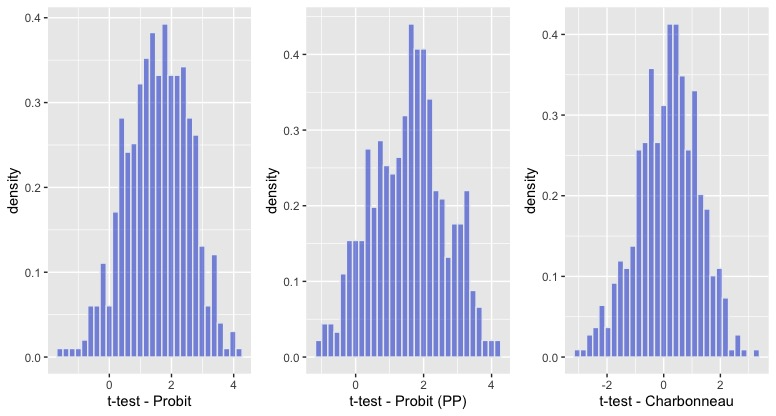
\includegraphics[scale=.4]{content/Figures/ttest_beta21_Design5.png}}
  \caption{\footnotesize{Histogram of the \textit{t-test} for estimated $\beta_{21}^*$ in Design 5}}
  \label{ttest_beta21_Design5}
\end{figure}
\begin{figure}
  \centerline{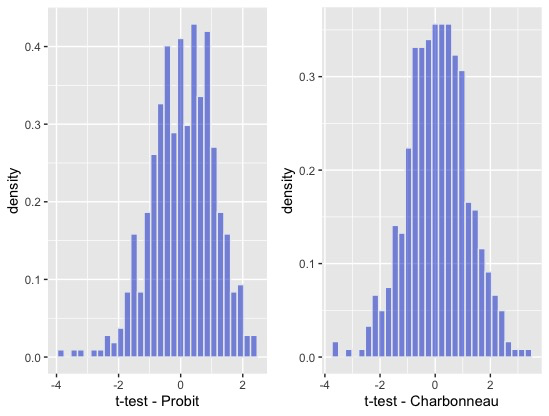
\includegraphics[scale=.4]{content/Figures/ttest_beta21_Design6.png}}
  \caption{\footnotesize{Histogram of the \textit{t-test} for estimated $\beta_{21}^*$ in Design 6}}
  \label{ttest_beta21_Design6}
\end{figure}
\begin{figure}
  \centerline{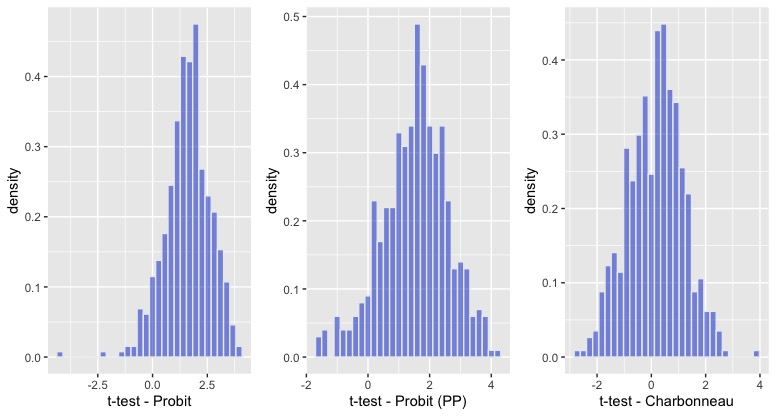
\includegraphics[scale=.4]{content/Figures/ttest_beta21_Design7.png}}
  \caption{\footnotesize{Histogram of the \textit{t-test} for estimated $\beta_{21}^*$ in Design 7}}
  \label{ttest_beta21_Design7}
\end{figure}
\begin{figure}
  \centerline{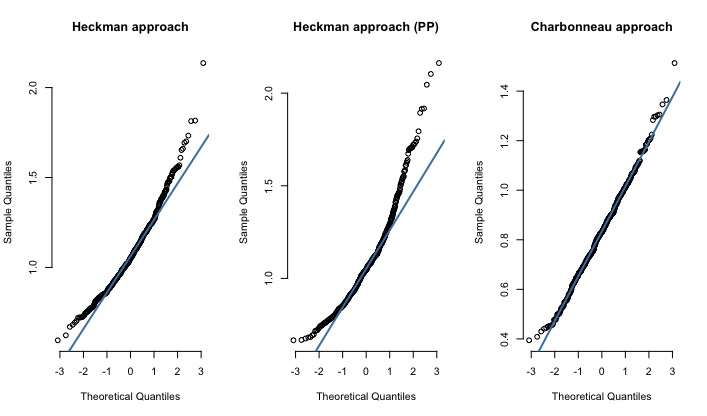
\includegraphics[scale=.4]{content/Figures/QQ_beta_21_Design5.png}}
  \caption{\footnotesize{QQ plot of estimated $\beta_{21}^*$ in Design 5}}
  \label{QQ_beta_21_Design5}
\end{figure}
\begin{figure}
  \vspace{-2.5em}%
  \centerline{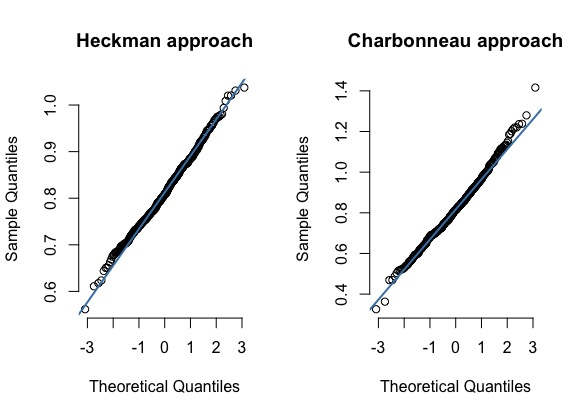
\includegraphics[scale=.4]{content/Figures/QQ_beta_21_Design6.png}}
  \caption{\footnotesize{QQ plot of estimated $\beta_{21}^*$ in Design 6}}
  \label{QQ_beta_21_Design6}
\end{figure}
\begin{figure}
  \vspace{-2.5em}%
  \centerline{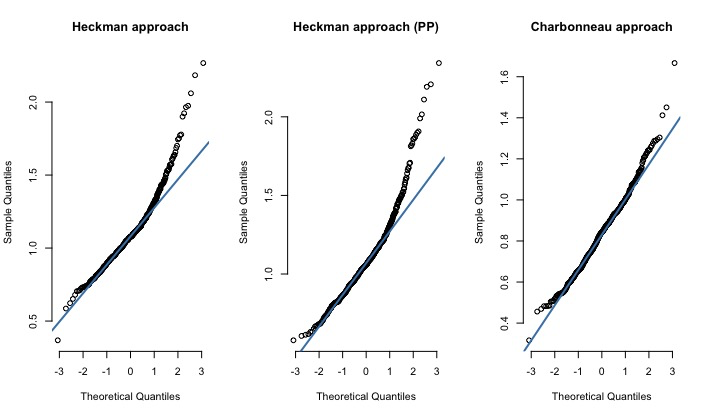
\includegraphics[scale=.4]{content/Figures/QQ_beta_21_Design7.png}}
  \caption{\footnotesize{QQ plot of estimated $\beta_{21}^*$ in Design 7}}
  \label{QQ_beta_21_Design7}
\end{figure}

The biases of the Probit and Probit (PP) estimators are also evident through the histogram for the \textit{t-tests} of the estimated $\beta_{21}^*$. For this analysis we focus on Designs 5, 6 and 7, which includes cases where the fixed effects are correlated with $x_1$, and the improvements of Charbonneau are the bigger. In Design 6, where there are no fixed effects, the distribution of both Probit and Charbonneau \textit{t-tests} are centered around zero, as illustrated in Figure \ref{ttest_beta21_Design6}, indicating that the tests have the right size. Also, from the shape of the distribution it indicates further that the estimated parameters are normally distributed. When there are fixed effects (Designs 5 and 7, in Figures \ref{ttest_beta21_Design5} and \ref{ttest_beta21_Design7}), while the \textit{t-tests} for Charbonneau are centered around zero, the ones for the Probit and Probit (PP) are not, indicating that the estimates are biased and the \textit{t-tests} do not have the correct size. 

The test sizes are also improved by the Charbonneau estimator. The significance level of the Probit and Probit (PP) estimators are much larger than 5\%, in most cases ranging between 20\% and 40\%. 

The distribution of the estimates are further assessed through the QQ-plots in Figures \ref{QQ_beta_21_Design5} - \ref{QQ_beta_21_Design7}. In Design 6, the plot indicates that the distributions for both estimators are reasonably well approximated by a normal distribution. In Designs 5 and 7, while the Charbonneau estimates the distributions are also well approximated by a normal, the Probit and Probit (PP) estimates have distributions that are more skewed. The same argument holds for the estimates of $\beta_{22}^*$ and $\beta_{23}^*$, which graphs are in the Appendix \ref{appendix_tables_figures}.
\begin{figure}
  \vspace{-2.5em}%
  \centerline{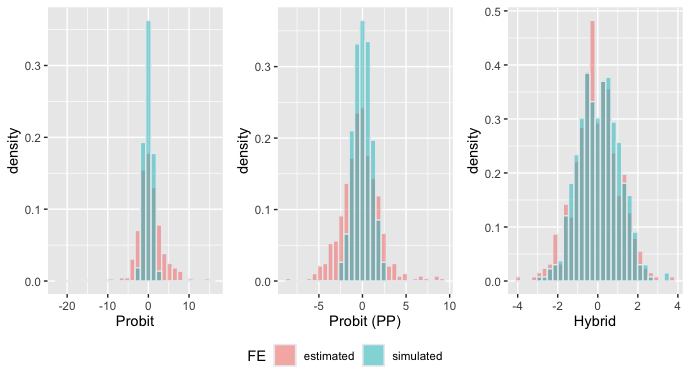
\includegraphics[scale=.45]{content/Figures/Hist_FE_Design5.png}}
  \caption{\footnotesize{Histogram of estimated $\xi_1^*$ in Design 5}}
  \label{fig}
\end{figure}
\begin{figure}
  \vspace{-2.5em}%
  \centerline{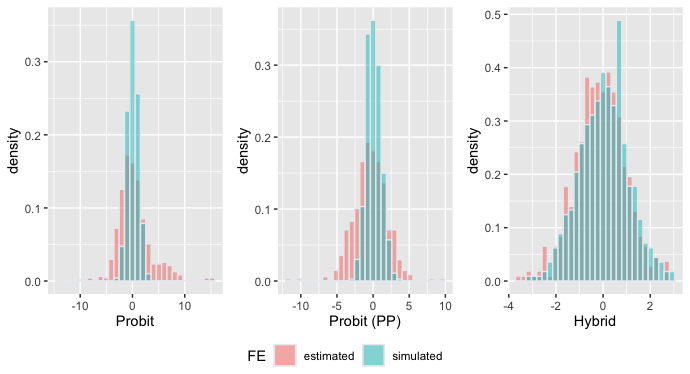
\includegraphics[scale=.45]{content/Figures/Hist_FE_Design7.png}}
  \caption{\footnotesize{Histogram of estimated $\xi_1^*$ in Design 7}}
  \label{fig}
\end{figure}

We now analyze the estimated fixed effects $\xi_i^*$ for $i=1$ throughout the simulations. For both Designs 5 and 7, the estimates obtained by the Hybrid approach are much more closely distributed to the true fixed effects than the Probit and Probit (PP) estimates. The Probit estimates are off due to two reasons: (i) they are not corrected for the perfect prediction problem, leading to extreme estimated values; and (ii) even for not extreme estimated values, the distributions are not similar once the estimates are contaminated by the (asymptotic) bias of the structural parameters. The latter problem is evidenced when we look at the estimates of the fixed effects for the Probit (PP) estimator. While the estimates vary over a smaller range once we correct for the perfect prediction problem, leading to less biased estimates in general for the fixed effects, their distribution is still quite different from the distribution of its true values, still presenting a larger range than the true distribution. This indicates that even when correcting for the perfect prediction, the estimates of the fixed effects are still contaminated by the bias in the structural parameters. In Tables \ref{tab:1} - \ref{tab:3} we can see that the estimates of both fixed effects $\xi_i^*$ and $\zeta_j^*$ have, in general, a much higher bias in the Probit estimators than in the Hybrid.
\begin{figure}[htbp]
  \centerline{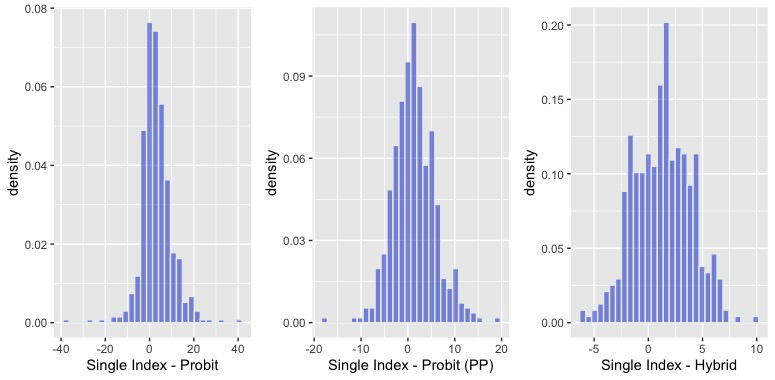
\includegraphics[scale=.4]{content/Figures/Hist_Zij_Design5.png}}
  \caption{\footnotesize{Histogram of $\hat{z}_{12} - z_{12}$ in Design 5}}
  \label{Hist_Zij_Design5}
\end{figure}
\begin{figure}[htbp]
  \centerline{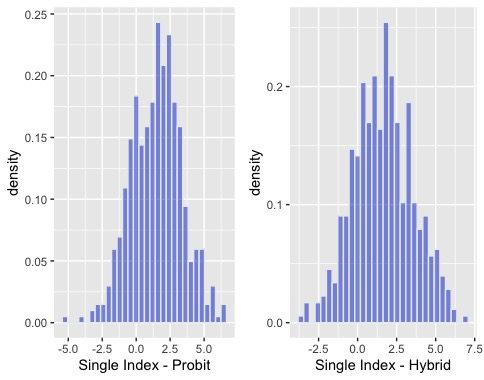
\includegraphics[scale=.4]{content/Figures/Hist_Zij_Design6.png}}
  \caption{\footnotesize{Histogram of $\hat{z}_{12} - z_{12}$ in Design 6}}
  \label{Hist_Zij_Design6}
\end{figure}
\begin{figure}[htbp]
  \centerline{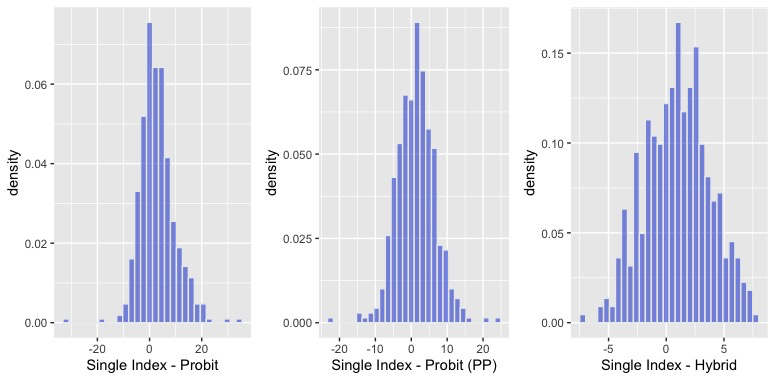
\includegraphics[scale=.4]{content/Figures/Hist_Zij_Design7.png}}
  \caption{\footnotesize{Histogram of $\hat{z}_{12} - z_{12}$ in Design 7}}
  \label{Hist_Zij_Design7}
\end{figure}
\begin{figure}[htbp]
  \centerline{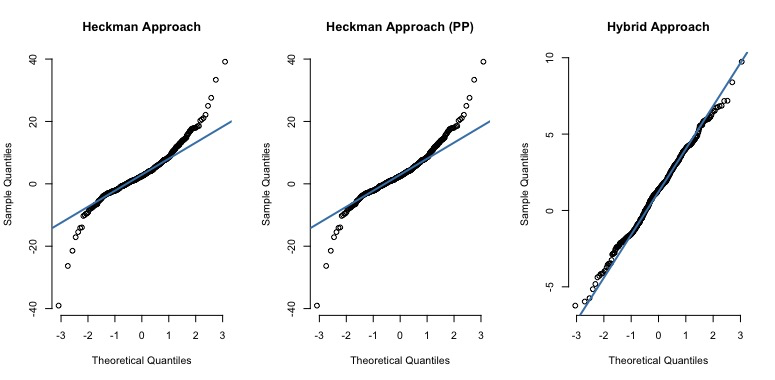
\includegraphics[scale=.4]{content/Figures/QQ_Zij_Design5.png}}
  \caption{\footnotesize{QQ plot of $\hat{z}_{12} - z_{12}$ in Design 5}}
  \label{QQ_Zij_Design5}
\end{figure}
\begin{figure}[htbp]
  \centerline{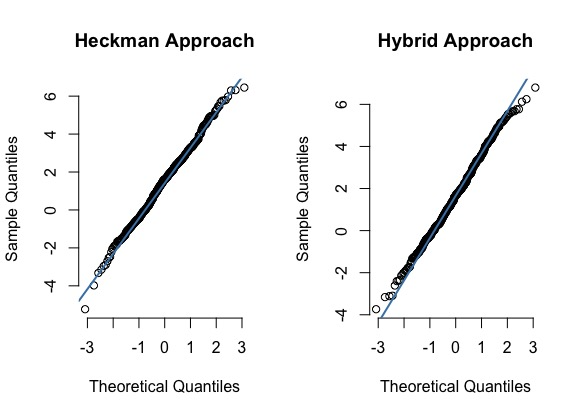
\includegraphics[scale=.4]{content/Figures/QQ_Zij_Design6.png}}
  \caption{\footnotesize{QQ plot of $\hat{z}_{12} - z_{12}$ in Design 6}}
  \label{QQ_Zij_Design6}
\end{figure}
\begin{figure}[htbp]
  \centerline{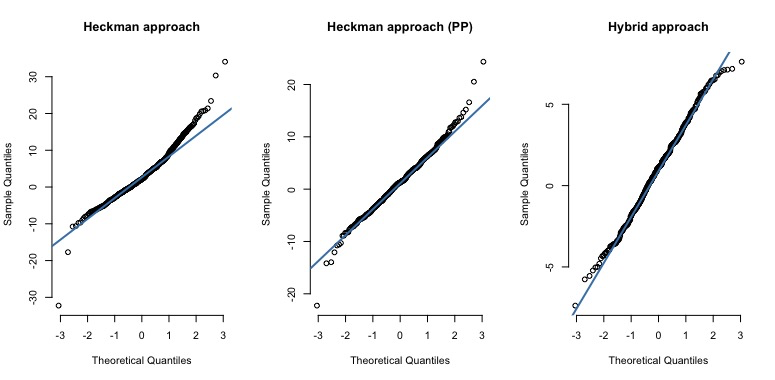
\includegraphics[scale=.4]{content/Figures/QQ_Zij_Design7.png}}
  \caption{\footnotesize{QQ plot of $\hat{z}_{12} - z_{12}$ in Design 7}}
  \label{QQ_Zij_Design7}
\end{figure}
\newline
Both the structural and fixed effects parameters estimated by the Probit and Probit (PP) are biased when fixed effects are present in the DGP. The structural parameters through the incidental parameters problem, and the fixed effects parameters through the biased carried over from the estimation of the $\beta_2^*$'s and through the perfect prediction problem in the Probit. Both sources of biases are carried over to the estimates of the single index $z_{ij}$. This is seen in the previous tables, where in the designs with fixed effects, the bias of the estimates of $z_{ij}$ are generally much larger for the Probit and Probit (PP). Even though the Probit (PP) produces less bias compared to the Probit estimator, since the perfect prediction problem is corrected, for most designs (with the exception of Design 7) the biases in the index $z_{ij}$ are still larger than that of the Hybrid approach.

We can also see that through the histograms of the quantities $\hat{z}_{12} - z_{12}$, i.e, the difference of the estimated single index for the dyad $i=1, j=2$ and its true value, given by Figures \ref{Hist_Zij_Design5} - \ref{Hist_Zij_Design7} . For Designs 5 and 7, the range of the histograms for the Probit estimates is much larger than that of the Probit (PP) or the Hybrid estimates. The Hybrid estimator presents an even lower range than the Probit (PP). In the case where fixed effects are not present, in Design 6, this is not true anymore.

Besides, the QQ-plots for such quantities, given by Figures \ref{QQ_Zij_Design5} - \ref{QQ_Zij_Design7}, show that in cases where there are fixed effects, the distribution of estimated single index for the Probit and the Probit (PP) are not well approximated by a normal, whereas for the Hybrid it is. There are two sources for that problem: (i) the fact that the structural parameters estimated by the Probit have a more skewed distribution than a normal, and (ii) the very extreme values estimated by the fixed effects. While the latter is aliviated for the Probit (PP) estimator, we notice that the estimations of the fixed effects are still varying over a wider range than those of the Hybrid approach. The QQ-plots indicates that for Design 5, the latter source dominates (as the figure indicates that the distribution of the single index has heavy tails), while for Design 7, the former source dominates. In the case of no fixed effects, all estimates are well behaved. 


\subsection{Second stage (estimation of the observation equation)}

In this section, we present the results obtained from the Monte Carlo simulations for the second stage (observations equation). We denote by Heckman the estimators obtained through the standard approach, that take into account the Probit estimates in the first stage. Analogously, we denote by Heckman (PP) the estimators given by the standard approach, taking into account the Probit (PP) estimates in the first stage (we employ this estimator only in designs where there are fixed effects in the selection equation). We denote by Hybrid the estimators obtained by using the transformation proposed by \cite{lee1983generalized}, and finally we denote by Kyriazidou the estimators obtained through our modified methodology based on \cite{kyriazidou1997estimation}.

As we still do not have an analytical expression for the standard errors of the latter two estimators, we will present only the mean bias and the mean standard deviation of the estimators. Moreover, for the Kyriazidou approach we also provide the estimators obtained through the asymptotic bias correction highlighted in Section \ref{bandwidth}, and we denote them by Kyriazidou(corrected). Following the parameters chosen in the simulations in \cite{kyriazidou1997estimation}, we set $r=1$ and $\delta = 0.1$. We choose the kernal density to be a standard normal density, and we experiment with several values of $h$, and its asymptotically bias corrections counterparts.

These results can be seen in Tables \ref{tab:6} and \ref{tab:7} for the seven proposed designs. 

\begin{table}
\begin{adjustwidth}{-.5in}{-.5in}
\vspace{-2.5em}%
\small
\centering
\begin{tabular}{p{3cm}p{1.3cm}p{1.3cm}p{1.3cm}p{1.3cm}p{1.3cm}p{1.3cm}p{1.3cm}}
  \hline
   \quad & Design 1 & Design 2 & Design 3 & Design 4 & Design 5 & Design 6 & Design 7  \\
   \hline
   \multicolumn{8}{l}{Heckman} \\
   \hline
    $\beta_{11}$  & 0.0002 (0.0482) & 0.0092 (0.0466) & 0.0014 (0.0527) & 0.0204 (0.0516) & 0.0160 (0.0343) & 0.0025 (0.0536) & 0.0161 (0.0573) \\
    $\beta_{12}$  & -0.0004 (0.0628) & -0.0257 (0.0612) & 0.0018 (0.0957) &  0.0288 (0.1063)& -0.0398 (0.0687) & -0.0025 (0.1005) & 0.0204 (0.1114) \\
    Inverse Mills-Ratio  & 0.0038 (0.1203)  & 0.0613 (0.1268) & 0.0037 (0.1659) & 0.1317 (0.1732) & 0.0606 (0.1387) & 0.0043 (0.1754) & 0.1310 (0.1877) \\
     & & & & & & & \\
    \hline
    \multicolumn{8}{l}{Heckman Perfect Prediction} \\
    \hline
     $\beta_{11}$  & & 0.0174 (0.0531) &  & 0.0291 (0.0628) & 0.0427 (0.0399) &  & 0.0246 (0.0645)\\
     $\beta_{12}$  & & -0.0495 (0.08513) &  & 0.0426 (0.1131)& -0.0676 (0.0871) &  & 0.0418 (0.1218)\\
     Inverse Mills-Ratio  & & -0.0997 (5.1842)&  & 0.1318 (2.7994) & 0.1016 (1.9824) &  & 0.4240 (4.0759)\\
      & & & & & & & \\
     \hline
   \multicolumn{8}{l}{Hybrid} \\
   \hline
    $\beta_{11}$  & -0.0049 (0.0587) & 0.0109 (0.0764) & 0.0001 (0.0705)& 0.0128 (0.0766) & 0.0119 (0.0925) & 0.0035 (0.0787)  & 0.0136 (0.0987)\\
    $\beta_{12}$  & 0.0001 (0.0854) &  0.0183 (0.1381) & 0.0038 (0.1304)& -0.0044 (0.1475) & 0.0150 (0.1601) & 0.0048 (0.1372) & -0.0051 (0.1743)\\
    Inverse Mills-Ratio  & 0.0050 (0.1332) &  0.0887 (0.2597) & 0.0189 (0.2644) & 0.0716 (0.2695) & 0.0968 (0.3198) & 0.0288 (0.2742) & 0.0781 (0.3329)\\
     & & & & & & & \\
    \hline
    \multicolumn{8}{l}{Kyriazidou $h=0.5$} \\
   \hline
    $\beta_{11}$  & -0.0093 (0.0820) & -0.0065 (0.0891) & -0.0071 (0.0811) & -0.0059 (0.0840) & -0.0058 (0.0941) & -0.0056 (0.0870) & -0.0052 (0.0903)\\
    $\beta_{12}$  & -0.0063 (0.1421) & -0.0022 (0.1465) & -0.0026 (0.1412) & -0.0072 (0.1494) &  0.0044 (0.1657) &  0.0031 (0.1557) & -0.0224 (0.1633)\\
     & & & & & & & \\
    \hline
    \multicolumn{8}{l}{Kyriazidou $h=0.5$, corrected} \\
   \hline
    $\beta_{11}$  & -0.0093 (0.0823) & -0.0066 (0.0894) & -0.0071 (0.0814) &  -0.0059 (0.0843) & -0.0058 (0.0944) & -0.0056 (0.0873) & -0.0053 (0.0907) \\
    $\beta_{12}$  & -0.0064 (0.1425) & -0.0022 (0.1471) & -0.0026 (0.1418) &  -0.0071 (0.1499) & 0.0044 (0.1664) &  0.0030 (0.1563) & -0.0225 (0.1640)\\
     & & & & & & & \\
    \hline
    \multicolumn{8}{l}{Kyriazidou $h=1$} \\
   \hline
    $\beta_{11}$  & -0.0081 (0.0736) & -0.0055 (0.0803) & -0.0069 (0.0729) & -0.0059 (0.0746) & -0.0057 (0.0862) &  -0.0057 (0.0790)& -0.0040 (0.0809)\\
    $\beta_{12}$  & -0.0039 (0.1290) & -0.0012 (0.1327) & -0.0017 (0.1264) & -0.0101 (0.1337)  & 0.0034 (0.1461) &  0.0019 (0.1391) & -0.0195 (0.1445)\\
     & & & & & & & \\
        \hline
    \multicolumn{8}{l}{Kyriazidou $h=1$, corrected} \\
   \hline
    $\beta_{11}$  & -0.0082 (0.0738) & -0.0056 (0.0805) & -0.0071 (0.0731) &  -0.0060 (0.0748) & -0.0058 (0.0864) & -0.0058 (0.0792) & -0.0041 (0.0812)\\
    $\beta_{12}$  & -0.0041 (0.1294) & -0.0013 (0.1331) & -0.0018 (0.1267) &  -0.0102 (0.1341) & 0.0033 (0.1465) &  0.0017 (0.1395) & -0.0197 (0.1449)\\
     & & & & & & & \\
    \hline
\end{tabular}
\caption{\footnotesize{Simulation results for the estimated coefficients for the observation Equation \ref{eq:dgp1} with $N=25$ and 500 iterations. The values correspond to the mean bias of estimates, and the standard deviation is in parenthesis. The estimator Heckman Perfect Prediction is only obtained for designs with fixed effects in the selection equation.}}
\label{tab:6}
\end{adjustwidth}
\end{table}
\begin{table}
\begin{adjustwidth}{-.5in}{-.5in}
\small
\centering
\begin{tabular}{p{3cm}p{1.3cm}p{1.3cm}p{1.3cm}p{1.3cm}p{1.3cm}p{1.3cm}p{1.3cm}}
  \hline
   \quad & Design 1 & Design 2 & Design 3 & Design 4 & Design 5 & Design 6 & Design 7  \\
   \hline
    \multicolumn{8}{l}{Kyriazidou $h=2$} \\
   \hline
    $\beta_{11}$  & -0.0070 (0.0692) & -0.0045 (0.0751) & -0.0063 (0.0690) &  -0.0044 (0.0701) & -0.0045 (0.0812) & -0.0051 (0.0735) & -0.0035 (0.0750)\\
    $\beta_{12}$  & -0.0017 (0.1210) & 0.0000 (0.1240) & -0.0021 (0.1175) & -0.0135 (0.1253) & 0.0039 (0.1371) &  0.0030 (0.1287) & -0.0175 (0.1346)\\
    & & & & & & & \\
    \hline
    \multicolumn{8}{l}{Kyriazidou $h=2$, corrected} \\
   \hline
    $\beta_{11}$  & -0.0073 (0.0694) & -0.0049 (0.0753) & -0.0066 (0.0692) &  -0.0048 (0.0703) & -0.0048 (0.0814) & -0.0055 (0.0737) & -0.0037 (0.0753) \\
    $\beta_{12}$  & -0.0022 (0.1213) & 0.0001 (0.1243) & -0.0026 (0.1177) &  -0.0138 (0.1256) & 0.0035 (0.1374) &  0.0026 (0.1290) & -0.0178 (0.1349) \\
         & & & & & & & \\
    \hline
    \multicolumn{8}{l}{Kyriazidou $h=3$} \\
   \hline
    $\beta_{11}$  & -0.0064 (0.0678) & -0.0037 (0.0731) & -0.0059 (0.0676) & -0.0032 (0.0682) & -0.0037 (0.0791) &  -0.0043 (0.0710) & -0.0028 (0.0722) \\
    $\beta_{12}$  & 0.0000 (0.1178) & 0.0000 (0.1205) & -0.0020 (0.1142) & -0.0142 (0.1218) & 0.0048 (0.1331) &  0.0043 (0.1246) & -0.0157 (0.1302)\\
    & & & & & & & \\
    \hline
    \multicolumn{8}{l}{Kyriazidou $h=3$, corrected} \\
   \hline
    $\beta_{11}$  & -0.0069 (0.0680) & -0.0042 (0.0734) & -0.0065 (0.0678) &  -0.0037 (0.0684) & -0.0041 (0.0794) & -0.0048 (0.0713) & -0.0032 (0.0724) \\
    $\beta_{12}$  & -0.0001 (0.1181) & -0.0010 (0.1208) & -0.0028 (0.1145) &  -0.0148 (0.1221) & 0.0043 (0.1334) &  0.0037 (0.1249) & -0.0162 (0.1305)\\
             & & & & & & & \\
    \hline
    \multicolumn{8}{l}{Kyriazidou $h=5$} \\
   \hline
    $\beta_{11}$  & -0.0044 (0.0658) & -0.0013 (0.0711) & -0.0039 (0.0656) & -0.0001 (0.0663) & -0.0020 (0.0768) & -0.0023 (0.0683) & -0.0014 (0.0693)\\
    $\beta_{12}$  & 0.0033 (0.1142) & 0.0010 (0.1167) & 0.0000 (0.1115) &  -0.0130 (0.1186) & 0.0071 (0.1286) & 0.0066 (0.1204) & -0.0124 (0.1262) \\
    & & & & & & & \\
    \hline
    \multicolumn{8}{l}{Kyriazidou $h=5$, corrected} \\
   \hline
    $\beta_{11}$  & -0.0052 (0.0661) & -0.0019 (0.0713) & -0.0047 (0.0659) &  -0.0016 (0.0666) & -0.0025 (0.0771) & -0.0030 (0.0685) & -0.0019 (0.0695) \\
    $\beta_{12}$  &  0.0023 (0.1146) & 0.0000 (0.1171) & -0.0011 (0.1118) &  -0.0138 (0.1189) & 0.0064 (0.1289) & 0.0057 (0.1208) & -0.0130 (0.1266) \\
                 & & & & & & & \\
    \hline
    \multicolumn{8}{l}{Kyriazidou $h=10$} \\
   \hline
    $\beta_{11}$  & 0.0045 (0.0614) & 0.0073 (0.0668) & 0.0056 (0.0617) &  0.0074 (0.0630) & 0.0043 (0.0722) &  0.0062 (0.0637) & 0.0045 (0.0656) \\
    $\beta_{12}$  & 0.0153 (0.1089) & 0.0113 (0.1116) & 0.0108 (0.1071) &  -0.0039 (0.1141) & 0.0156 (0.1226) & 0.0168 (0.1144) & -0.0046 (0.1210)\\
    & & & & & & & \\
    \hline
    \multicolumn{8}{l}{Kyriazidou $h=10$, corrected} \\
   \hline
    $\beta_{11}$  & 0.0036 (0.0616) & 0.0066 (0.0670) & 0.0047 (0.0619) &  0.0067 (0.0632) & 0.0038 (0.0725) &  0.0054 (0.0640)& 0.0040 (0.0658) \\
    $\beta_{12}$  & 0.0142 (0.1092) & 0.0104 (0.1119) & 0.0097 (0.1074) &  -0.0048 (0.1144) & 0.0150 (0.1229) &  0.0158 (0.1147) & -0.0052 (0.1213)\\
    \hline
\end{tabular}
\caption{\footnotesize{Simulation results for the estimated coefficients for the observation Equation \ref{eq:dgp1} with $N=25$ and 500 iterations. The values correspond to the mean bias of estimates, and the standard deviation is in parenthesis.}}
\label{tab:7}
\end{adjustwidth}
\end{table}

We can see that for designs where there were no fixed effects in the selection equation (Designs 1, 3 and 6) all proposed estimators present essentially no bias. The exceptions are given by (i) the estimates of the coefficient of the inverse Mills-ratio (which true value is essentially the correlation between the errors in the equations) in the Hybrid approach, and (ii) the estimates of $\beta_{12}$ given by the Kyriazidou and Kyriazidou(corrected) estimators for $h=10$. The latter is expected, since, as argued by \cite{kyriazidou1997estimation}, the bias of the estimates increases when the chosen bandwidth is increased.

The fact that such estimates are mostly unbiased for all proposed estimators also points out that even when fixed effects in the observation equation are present (as in Designs 3 and 6), the methods that rely on including dummy variables for them, namely, Heckman and Hybrid, deliver estimates with nice properties. Moreover, in this case, Kyriazidou, which relies on differencing out those fixed effects together with the sample selection effects also performs well. However, notice that the precision of the Hybrid and Kyriazidou approaches are slightly lower than the Heckman approach. 

When fixed effects in the selection equation are included (Designs 2, 4, 5, 7), the Heckman and Heckman (PP) estimators present biases, which is aligned with Theorem \ref{theorem_heckman}. Since the single indices are biased in such cases, the estimates of the observation equation are likely to be also biased. Such biases are more pronounced for the coefficient of the binary variable $x_{2}$. Also, for this variable, the biases are not always in the same direction. However, it is striking that when comparing both estimators, the Heckman (PP) delivers even more biased estimates.

We note that for such designs, the Hybrid approach reduces the biases in general, specially for the coefficient of the binary variable. However, for Designs 2, 4 and 5, the Kyriazidou and Kyriazidou(corrected) estimators reduces the biases even further, specially for the initial choice of $h$ ranging between 0.5 and 5. Moreover, looking at the standard deviations, in general, the Kyriazidou estimators reduce the bias while not sacrificing precision.

The exception to this observation is in Design 7. For this design we have that, while Kyriazidou estimators reduce further the biases in the coefficients of the continuous regressor $x_1$, the Hybrid approach does a better job for the binary variable $x_2$. For the coefficients of this variable the Kyriazidou estimators only reduces the biases observed in the Heckman estimator for $h>2$. Then, the bias is basically eliminated only for $h=10$. This contradicts the argument of \cite{kyriazidou1997estimation} that the bias of the estimates increases when the chosen bandwidth is increased. Also, it points out that the estimates are sensitive to the choice of the initial $h$.However, note that the Kyriazidou estimators always reduces the biases when compared to the Heckman (PP) estimator, for all the designs and all the initially chosen values of $h$.

In appendix \ref{appendix_tables_figures} the estimates for all designs and approaches are given such that the parameters of the first stage estimation are set to their true value (for the Hybrid approach it boils down to only applying Lee's transformation on the variables). We note that in this case, the Kyriazidou estimators delivers unbiased estimates for all designs (except for the case when $h=2$). Therefore, there is evidence that such remaining biases might come from the estimators of the first stage. We saw previously that the biases in the first stage Charbonneau estimates still did not vanish due to the reduced sample size. This indicates that possibly the remaining biases seen here are not originated by the Kyriazidou estimator itself. An intriguing fact is that the Hybrid estimator in this case presents some bias for the estimate of $\beta_{12}$.

Moreover, from the tables we can see that the estimators provided by Kyriazidou(corrected) do not reduce biases further compared to Kyriazidou. Even though that is contractory to Corollary \ref{corollary}, the same is observed in the simulations provided in \cite{kyriazidou1997estimation}. There are two possible explanations for this: (i) the small sample bias is more important than the asymptotic bias for these designs, or (ii) other methods for choosing an appropriate bandwith given an initial chosen $h$ should be provided.
\begin{figure}[htbp]
  \vspace{-2.5em}%
  \centerline{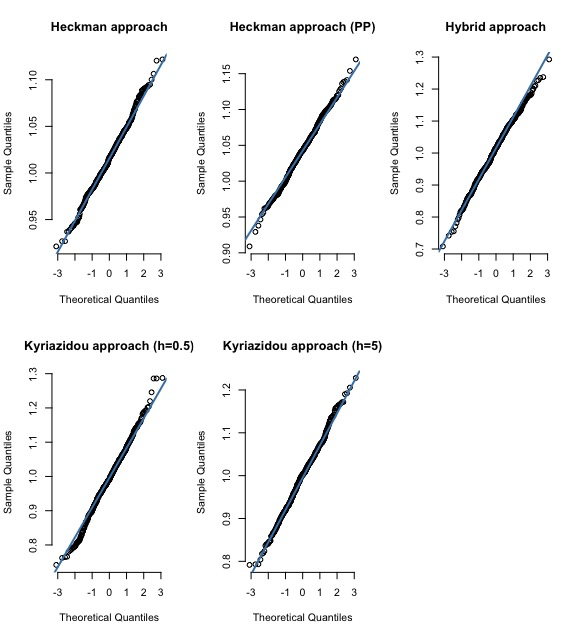
\includegraphics[scale=.4]{content/Figures/QQ_beta_11_Design5.png}}
  \caption{\footnotesize{QQ plot of estimated $\beta_{11}$ in Design 5}}
  \label{QQ_beta_11_Design5}
\end{figure}
\begin{figure}[htbp]
  \vspace{-2.5em}%
  \begin{adjustwidth}{-.5in}{-.5in}
  \centerline{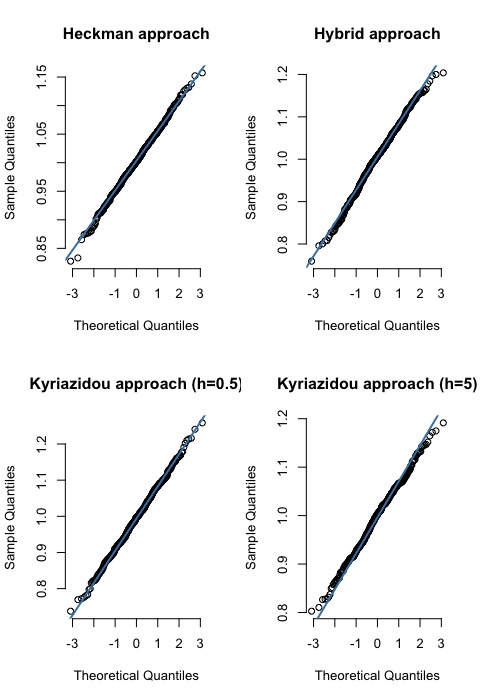
\includegraphics[scale=.4]{content/Figures/QQ_beta_11_Design6.png}}
  \caption{\footnotesize{QQ plot of estimated $\beta_{11}$ in Design 6}}
  \label{QQ_beta_11_Design6}
  \end{adjustwidth}
\end{figure}
\begin{figure}[htbp]
  \vspace{-2.5em}%
  \begin{adjustwidth}{-.5in}{-.5in}
  \centerline{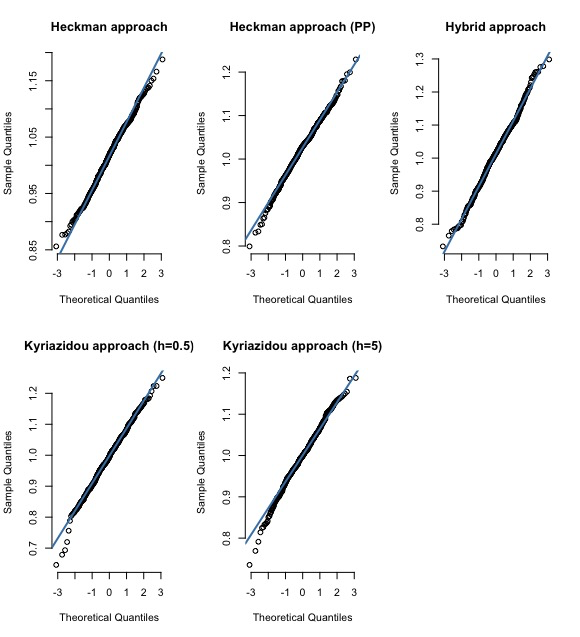
\includegraphics[scale=.4]{content/Figures/QQ_beta_11_Design7.png}}
  \caption{\footnotesize{QQ plot of estimated $\beta_{11}$ in Design 7}}
  \label{QQ_beta_11_Design7}
  \end{adjustwidth}
\end{figure}

In Figures \ref{QQ_beta_11_Design5} - \ref{QQ_beta_11_Design7}, we provide the QQ-plots for the estimates obtained by the different approaches for the parameter $\beta_{11}$. While it is expected that the estimates of the Hybrid and the Kyriazidou approaches are approximatelly normal, it is striking that the estimates of the Heckman methods are also approximately normally distributed, since the distribution of single indexes for these approaches deviates from a normal distribution. The same is observed for the estimates of the parameter $\beta_{12}$, which plots are presented in Appendix \ref{appendix_tables_figures}.


\section{An application to the gravity model for international trade} \label{application}

In this section we apply the proposed methods for estimating gravity models to international trade flows. We aim to estimate how trade barriers affect both the decision of country $i$ to export to country $j$, and the volume of trade. We will estimate the model outlined in Section \ref{estimating_helpman}, with the only difference being that we do not include $w_{ij}$ as a regressor in the second stage estimation. This variable accounts for the fraction of firms that export from country $i$ to country $j$ in country $i$, being related to the extensive margins of trade. When this variable is omitted, the estimation confounds the effects of trade barriers on the intensity  of trade (intensive margin) with the effects on the proportion of exporting firms (extensive margin). The sample selection effect is introduced in this model when only countries with positive trade flows are taken into account in the observation equation.

Therefore, while the estimation proposed by \cite{helpman2008estimating} corrects both for the effect of this variable $w_{ij}$ and the sample selection effect in the observation equation, we will focus here on the latter effect. 

The reason to not take into account $w_{ij}$ for now is that this is an estimated variable, that is obtained through the estimated inverse Mills-ratio. As demonstrated in \cite{helpman2008estimating}, it introduces a further non-linearity in the observation equation. This non-linearity needs to be taken into account by employing a non-linear least squares (NLS) estimator when applying the standard Heckman approach. Therefore, for simplicity, and to clearly explore the differences between our proposed estimators and the standard Heckman procedure, we will focus only on correcting for the sample selection bias.

We use the dataset provided by \cite{helpman2008estimating}, which is the same used by \cite{charbonneau2017multiple} in her application to estimate the parameters for the first stage estimation, that refers to the decision of countries to trade (the probability that country $i$ exports to country $j$). Therefore, we can compare our results in the first stage estimation with both results obtained by \cite{helpman2008estimating} and \cite{charbonneau2017multiple}, determining if we have a successfull replication of their studies.

The dataset provides information on directed trade flows and country characteristics for 158 countries in 1986. The country characteristics boil down to attributes on the country pairs (dyads). The variables used are, as described by \cite{helpman2008estimating}:

\begin{itemize}
    \item \textit{Distance}$_{ij}$: the distance (km) between the exporter's $i$ and importer's $j$ capitals in logs.
    \item \textit{Common Border}$_{ij}$: a binary variable that equals one if the exporter $i$ and importer $j$ share borders (are neighbors).
    \item \textit{Colonial ties}$_{ij}$: a binary variable that equals one if importing  country $j$ ever colonized in the history the exporting country $i$ or vice versa, and zero otherwise.
    \item \textit{Currency Union}$_{ij}$: a binary variable that equals one if the exporter $i$ and the importer $j$ have a common currency or if their own currencies had a 1:1 exchange rate for an extended period of time, and zero otherwise.
    \item \textit{Common Legal system}$_{ij}$: a binary variable that equals one if the exporting country $i$ and importing country $j$ have the same legal origin, and zero otherwise.
    \item \textit{Common Religion}$_{ij}$: $(\%$ Protestants in country $i$. \% Protestants in country $j$ ) $+(\%$ Catholics in country $i \cdot \%$ Catholics in country $j$ ) $+(\%$ Muslims in country $i$. \% Muslims in country $j$ ).
    \item \textit{FTA}$_{ij}$: a binary variable that equals one if the exporter $i$ and the importer $j$ belong to a common regional trade agreement, and zero otherwise.
\end{itemize}

In our estimation of the first stage equation we disconsider the observations with Congo as an exporter, as for those, the decision of trade does not change (Congo never exports to any country). This is done to avoid the problem of perfect predictability.

Both \cite{helpman2008estimating} and \cite{charbonneau2017multiple} take into account variables related to whether both countries are islands or if both do not have direct access to the sea. However, when we implement the Charbonneau approach in this application, such transformed variables lack of variation for the identification of the parameters. For obtaining the coefficients, we apply a standard logit estimation to the transformed variable (note that the standard errors have a more involved estimation, obtained as \cite{jochmans2018semiparametric} proposes). The reason why \cite{charbonneau2017multiple} is able to incorporate such variables might come from two sources: (i) instead of applying a standard logit, the author maximizes numerically the Equation (\ref{max_charb}), or (ii) the author takes into account the observations with Congo as exporter. However, this is not a crucial issue, once other studies also disregarded such variables (for instance, \cite{jochmans2018semiparametric}).

For more details on the construction of the variables in the dataset, refer to Appendix I in \cite{helpman2008estimating}.

We estimate the parameters $\beta_2^*$ of the following equation in the first stage (selection equation):
\begin{align}
    y_{2,i j}= \mathbbm{1}(x_{2,ij}'\beta_2^* +\xi_{i}^*+\zeta_{j}^* >\eta_{i j}^*)
    \label{eq:app1}
\end{align}

\noindent where: (i) $y_{2,i j}$ is a binary variable, being one if the $i$ exports to $j$ and zero otherwise, (ii) $\xi_{i}^*$ is the exporter fixed effect, (iii) $\zeta_{j}^*$ is the importer fixed effect, (iv) $x_{2,ij}$ is the vector that collects the variables \textit{Distance}$_{ij}$, \textit{Common Border}$_{ij}$, \textit{Colonial Ties}$_{ij}$, \textit{Currency Union}$_{ij}$, \textit{Common Legal System}$_{ij}$, \textit{FTA}$_{ij}$, \textit{Common Religion}$_{ij}$.

The following is the specified model for the second stage (observation equation):
\begin{align}
    y_{1,ij,t} = x_{1,ij,t}'\beta_1 + \vartheta_i + \chi_j + u_{ij,t}
    \label{eq:app2}
\end{align}

\noindent where: (i) $y_{1,ij}$ is the log of the value of the exports from $i$ to $j$, (ii) $\vartheta_i$ is the exporter fixed effect, (iii) $\chi_j$ is the importer fixed effect, (iii) $x_{1,ij,t}$ is the vector that collects the same variables as $x_{2,ij}$, with the exception of \textit{Common Religion}$_{ij}$ which is taken into account only in the first estimates of the standard Heckman approach as we will explain later. We only use dyads with positive exports to estimate this second stage equation. Therefore, a sample selection correction must be employed.

\subsection{Estimation of selection equation (decision to trade)}

We estimate the selection equation using a standard Probit with dummies for the fixed effects (which here boils down to the Probit (PP) in our simulations, as we excluded Congo as an exporter) and the Charbonneau estimator. The results can be seen in Table \ref{tab:app1}.
\begin{table}
    \small
    \centering
    \begin{tabular}{p{5cm}p{2cm}p{2cm}}
      \hline
       \quad & Probit  & Charbonneau \\
       \hline
        \textit{Common language}  &  $0.2903^{***}$ (0.0379) &  $0.4248^{***}$ (0.0732) \\
        \textit{Common legal system}  &  $0.0972^{**}$ (0.0296) &  $0.1822^{***}$ (0.0597)\\
        \textit{Common Religion} & $0.2647^{***}$ (0.0585)&  $0.4979^{***}$ (0.1125)\\
        \textit{Common Border} & $-0.3798^{***}$ (0.0946) &  $-0.5164^{**}$ (0.2300)\\
        \textit{Currency Union} &  $0.4883^{***}$ (0.1306) &  $1.0459^{***}$ (0.2362)\\
        \textit{Distance}  & $-0.6626^{***}$ (0.0208) &  $-1.0001^{***}$ (0.0541)\\
        \textit{FTA} &  $2.0170^{***}$ (0.3085) & $3.5565^{***}$ (0.5237)\\
        \textit{Colonial Ties} &  $0.3337$ (0.2852) &  $1.1432^{*}$ (0.6473)\\
         & &  \\
        \hline
    \end{tabular}
    \caption{\footnotesize{Estimates for the first stage Equation \ref{eq:app1}. For the Probit estimates we consider importer and exporter fixed effects, correcting for the perfect prediction problem. Standard errors are in parenthesis. \newline \textsuperscript{*} indicates that the coefficient is significant at the 10 \% level \newline \textsuperscript{**} indicates that the coefficient is significant at the 5 \% level \newline \textsuperscript{***} indicates that the coefficient is significant at the 1 \% level.}}
    \label{tab:app1}
\end{table}

Even though we do not take into account two variables considered by \cite{charbonneau2017multiple}, our estimates for the remaining parameters are remarkably similar for both estimators and for all remaining coefficients, when comparing to the results she presents in her paper.

We can see that our Charbonneau estimates have a higher magnitude for all the coefficients when compared to our Probit estimates. Thus, the proposed correction for the asymptotic biases in the standard Probit model plays a practical role in this application.

All the estimates also have the same sign as the ones obtained by \cite{helpman2008estimating} (where the Probit estimator is applied in the first stage). As expected, geographic distance decreases the probability of countries to trade, while the coefficients for the other characteristics that reflect how similar countries $i$ and $j$ are in general positive (\textit{Common Language}, \textit{Common Religion}, \textit{Colonial Ties}, \textit{Currency Union}, \textit{Common Legal System}), indicating that there is homophily in how trade networks are formed (similar countries have a higher propensity to trade). Countries that belong to a common regional trade agreement also have a higher probability of trading, as expected.

The estimates for both methods point out that countries with a common border are likely to trade less. As explained by \cite{helpman2008estimating}, this negative effect might be due to territorial border conflicts that harms trade between countries that are neighbors.

For the Charbonneau method, we estimate the standard errors as proposed by \cite{jochmans2018semiparametric}. Even though \cite{charbonneau2017multiple} does not clearly state how the estimates of the standard errors are obtained in her paper, when comparing, we find that our estimates are similar to hers. The exceptions are only for the variables \textit{Colonial Ties} and \textit{FTA}. In terms of significance levels, the variable \textit{FTA} is significant at the 1\% level both in our application and in hers, while the variable \textit{Colonial Ties} is not significant even at the 10\% level in her application and here it is significant at this level.

When comparing our Charbonneau estimates to our Probit estimates, the levels of significance of the variables are also very similar, with the exceptions of (i) \textit{Common legal system}, which in these estimations it is significant at the 5\% level, while in our Charbonneau estimation is significant at the 1\% level; and (ii) \textit{Colonial Ties}, which is not significant even at the 10\% level in the Probit estimations, but it is significant at this level for the Charbonneau estimator, as mentioned before.

\subsection{Estimation of observation equation (directed trade flows)}

Once the estimates of the first stage are obtained, we follow to the estimation of the second stage, which measures the effects of these variables on the volumes of exports from country $i$ to $j$. 

We apply the same methods outlined in Section \ref{simulations}. Namely, given the Probit estimates we employ the standard Heckman approach, and given the Charbonneau estimates, we employ the Hybrid and modified Kyriazidou approaches (with and without the asymptotic corrections). All the methods propose to correct for sample selectivity, and thus, allow for correlation between the errors of Equations (\ref{eq:app1}) and (\ref{eq:app2}).

For the modified Kyriazidou approach, we follow the parameters chosen in Section \ref{simulations}, setting $r=1$, $\delta = 0.1$, and experimenting throughout a range of possible values of the initial bandwidth $h$. Moreover, this approach requires a variable that satisfies an exclusion restriction in the sense that it affects the decisions to trade (affects the fixed costs of trading), but it does not affect the volume of trade flows (does not affect the variable costs). We follow \cite{helpman2008estimating} and use \textit{Common Religion} as such variable. That \textit{Common Religion} affects the decision of trade is clear from the estimates of the first stage. For the second requirement, the authors argue that when including variables related to regulation costs of firm entry, the coefficient of the variable \textit{Common Religion} becomes not significant in the second stage. Note that variables related to regulation costs satisfy the exclusion restriction, since by construction they do not affect the variable costs.

In this study, we deliberately chose not to include the variables that refer to the regulation costs, since they reduce the sample size drastically. In our case, this is aggravated since both the Charbonneau and the modified Kyriazidou estimators already reduce the amount of information used from the dataset due to all the conditions that must be met on quadruples.

However, as it is evident on the results presented in Table \ref{tab:app2}, the variable \textit{Common Religion} does not completely satisfy the conditions of exclusion restriction, since its coefficient in the estimates of the standard Heckman approach is still significant at the 5\% level. Thus, one should be careful when looking at the estimates of the modified Kyriazidou approach. We could not verify the significance level in the new proposed approaches since the estimates of the standard errors are still not available.
\begin{sidewaystable}
        \small
        \centering
        \begin{tabular}{p{4cm}p{1.8cm}p{1.8cm}p{1.8cm}p{1.8cm}p{1.8cm}p{1.8cm}p{1.8cm}p{1.8cm}p{1.8cm}}
          \hline
           \quad  &Heckman (1) & Heckman (2) &Hybrid  & K (h=0.5)  & K,corrected (h=0.5)  & K (h=1)  & K,corrected (h=1)\\
           \hline
            \textit{Common Language}  & $0.2090^{***}$ & $0.2333^{***}$& 0.3566 & 0.1094 & 0.1069&  0.1465& 0.1448\\
            \textit{Common Legal System}  & $0.4797^{***}$ & $0.4914^{***}$& 0.4975 & 0.3805& 0.3791& 0.4054& 0.4047\\
            \textit{Common Border}  & $0.4031^{***}$ & $0.4318^{***}$ & 0.5836& 0.6114 & 0.6127& 0.6106& 0.6131\\
            \textit{Currency Union}   & $1.3537^{***}$ & $1.3368^{***}$ & 1.4456 & 1.2315& 1.2248& 1.3186& 1.3158\\
            \textit{Distance}   & $-1.2087^{***}$ & $-1.2190^{***}$& -1.3470& -1.1371& -1.1329& -1.2185& -1.2187\\
            \textit{FTA}  &  $0.7774^{***}$ & $0.7719^{***}$& 2.0569 & 1.2835& 1.2835& 1.2475& 1.2636\\
            \textit{Colonial Ties}  & $1.3418^{***}$ & $1.3434^{***}$ & 1.4209 & 1.2594 &1.2560 & 1.3524& 1.3563\\
            \textit{Common Religion}  &  $0.2389^{**}$ &  &  &  &  &  & \\
            \textit{Inverse Mills-Ratio}  & $0.2784^{***}$ & $0.2671^{***}$ & 0.7130& & & &\\
             &  & & & & & &\\
            \hline
        \end{tabular}
        \caption{\footnotesize{Estimates for the second stage Equation \ref{eq:app2}. For the Heckman and Hybrid estimates we consider importer and exporter fixed effects, correcting for the perfect prediction problem. We denote by Kyriazidou by $K$. \newline \textsuperscript{*} indicates that the coefficient is significant at the 10 \% level \newline \textsuperscript{**} indicates that the coefficient is significant at the 5 \% level \newline \textsuperscript{***} indicates that the coefficient is significant at the 1 \% level.}}
        \label{tab:app2}
\end{sidewaystable}
\begin{sidewaystable}
    \begin{adjustwidth}{-.5in}{-.5in}
        \small
        \centering
        \begin{tabular}{p{4cm}p{1.8cm}p{1.8cm}p{1.8cm}p{1.8cm}p{1.8cm}p{1.8cm}p{1.8cm}p{1.8cm}p{1.8cm}}
          \hline
           \quad & K(h=2)  & K,corrected (h=2)  & K(h=3)  & K,corrected (h=3)  & K(h=5)  & K,corrected (h=5)  & K(h=10)  & K,corrected (h=10)\\
           \hline
            \textit{Common Language}  & 0.1696 & 0.1685 & 0.1830 & 0.1822& 0.1933& 0.1926& 0.1994& 0.1987\\
            \textit{Common Legal System}   & 0.4154 & 0.4151 & 0.4206 & 0.4204& 0.4242& 0.4240 & 0.4255& 0.4252\\
            \textit{Common Border}  & 0.5920 & 0.5950 & 0.5673 & 0.5708& 0.5436& 0.5486& 0.5129& 0.5193\\
            \textit{Currency Union}  & 1.4043 & 1.4035 & 1.4164& 1.4159& 1.3955& 1.3941& 1.4213& 1.4208\\
            \textit{Distance}  &  -1.2525& -1.2555 & -1.2503& -1.2538& -1.2172& -1.2198& -1.1721& -1.1730\\
            \textit{FTA} & 1.3033 & 1.3415 & 1.2408& 1.2826& 0.8675& 0.8972& 0.2901& 0.2981\\
            \textit{Colonial Ties} & 1.3729 & 1.3794 & 1.3387 & 1.3441& 1.2552& 1.2576& 1.1945& 1.1947\\
            &  &  &  & & & & & \\
            \hline
        \end{tabular}
        \caption{\footnotesize{Estimates for the second stage Equation \ref{eq:app2}. We denote by Kyriazidou by $K$. }}
        \label{tab:app3}
    \end{adjustwidth}
\end{sidewaystable}

From Tables \ref{tab:app2} and \ref{tab:app3}, we can see that regardless of the employed method, all coefficients except for \textit{Distance} are positive. In the case of the variable \textit{Common Border} this means that, while being neighbors reduces the probability of trading, when trade is made, being neighbors increases the volume of trade. 

The estimates obtained with the Hybrid and the modified Kyriazidou approach are different from the ones obtained with the standard Heckman approach. Thus, there is evidence that the latter is biased. However, we should point out that in order to properly claim that there are biases in the estimates, we would need to test whether the estimated coefficients are significantly different. As we still do not have estimates for the standard errors in the proposed approaches, this test cannot be done.

Moreover, while for some variables these possible biases have a clear direction when looking at the estimates provided by the two proposed methods, for others it does not have. 

The coefficient of \textit{Common Border} is higher for all estimates obtained from the Hybrid and the Kyriazidou approach. For the \textit{FTA} variable, the same holds, except for the estimator obtained with the Kyriazidou approach when setting the initial $h$ to be ten. Finally, for \textit{Currency Union} the coefficients are also higher for the Hybrid approach and for the Kyriazidou with higher levels of the initial $h$. For the remaining variables, the two proposed methods would imply various directions for the bias.

As in the results obtained in the simulation exercise, the asymptotic correction for the estimates of the modified Kyriazidou approach does not deliver different estimates compared to the initial estimation. Finally, it is evidenced in this application that the estimates for this approach are sensitive to the initial chosen level of $h$.



\section{Conclusion} \label{conclusion}
In this study we showed that accounting for sample selection bias in dyadic data settings is not straightforward and requires more involved methods than the standard \cite{helpman2008estimating} two-step approach. The standard Heckman approach involves a first stage where the probability of observing an outcome is estimated through a probit model with dummys for fixed effects, and a second stage that estimates the effects of different variables on such outcome, taking into account the estimated probabilities in the first stage.

The motivation to study dyadic interactions came from the gravity models for international flows. We specifically consider the model proposed by \cite{helpman2008estimating}, since it explicitly takes into account how the sample selectivity arises when estimating how trade barriers affect trade flows, when considering in the estimation only countries with positive trade flows. Another key aspect in this model is the presence of multilateral resistance terms, that boils down to the inclusion of two-way fixed effects for both countries involved in the trade.

Even though the motivation emerged from the trade literature, the approaches outlined in this study can be applied to any dyadic interaction where sample selectivity might be present (given that the model satisfies the outlined assumptions throughout the study). More generally, the first stage estimations, which outline the probability of observing a pairwise interaction that generates an outcome (in the case above, the probability of trading with each other), can be seen as an estimation of a network formation model, as highlighted in \cite{jochmans2018semiparametric}. The presence of the two-way fixed effects also indicates a close relationship to the $\beta$-models in the networks literature.

The difficulty in correcting for sample selectivity in such models arises as the two-way fixed effects are incorporated in the first stage estimation. These effects leads to the incidental parameter problem (\cite{neyman1948consistent}), and the estimates of structural parameters obtained through the standard Probit are asymptotically biased (\cite{fernandez2016individual}).

We showed more formally how this problem arises, and proposed the conditional logit estimates of \cite{charbonneau2017multiple} to estimate the structural parameters of the first stage equation. Such method relies on a clever way of differencing out both fixed effects in the equation over quadruples of dyads. The downside of this method is that it evidently does not provide estimates of the fixed effects, and therefore, the estimation of the inverse Mills-ratio for the traditional Heckman approach are not readily available.

To bypass this problem, we proposed two approaches based on existing methods, but providing the suitable modifications to this setting of dyadic regressions. The first method, denoted by Hybrid, relies on retrieving the estimates of the fixed effects through the unconditional log-likelihood, restricting the structural parameters to be the same as the estimates obtained by the Charbonneau estimates. Once the fixed effects estimates are collected, it is possible to transform the variables, as proposed by \cite{lee1983generalized} such that the Heckman two-step approach can be employed even when the errors in the selection equation are logistically distributed. The advantages of this approach is that there is no need for a variable that satisfies an exclusion restriction, since the sample selection effects have a defined functional form in the observation equation, guaranteeing the identification of its structural parameters. The downsides of this method are that (i) one still needs to obtain estimates for the fixed effects in the first stage equation, pointing out that this approach may not be suitable for sparse networks, and that (ii) the distribution of the errors need to be specified.

The second method is based on \cite{kyriazidou1997estimation}, and involves differencing the second stage equation over quadruples of dyads. The form of differencing guarantees that the fixed effects in the second stage equation are completely differenced out, however it does not guarantee that the sample selectivity effects are completely differenced out as well. To overcome this problem, the main idea is then that weights are applied to the transformed observations such that a higher weight is attributed to quadruples for which the differences in the sample selectivity effects are smaller. Such differences in sample selectivity effects take into account the estimates provided by Charbonneau of the first stage. The benefits of this method is that there is no need to estimate any of the fixed effects in both equations, and to specify the distribution of the errors in the observation equation. The deficiencies of this approach are that the estimates are sensitive to the choices of bandwidths $h$, as shown in the application and in the Monte Carlo simulations. Also, the proposed method to choose an optimal bandwidth seems to not show improvements. One aspect of both methods is that they are computationally costly, since they boil down to combinatoric problems over quadruples of dyads that must satisfy some given restrictions.

Our Monte Carlo simulation exercise confirms the theoretical predictions that under the normality assumption of both error terms, the estimators of the first stage equation given by the Probit model with fixed effects are biased. On top of that, such biases are carried over to the estimations of the second stage equation, given by the standard Heckman approach. The exercise also demonstrates that,as predicted by the theory, the proposed methods (under their respective assumptions) deliver reductions in the biases the estimators of both equations.

However, we must point out that in our empirical application to the gravity model for international trade flows, it is not straightforward to draw conclusions from the obtained estimates from the different approaches for some variables. One of the potential sources for this limitation is that the method based on \cite{kyriazidou1997estimation} requires a variable that satisfies an exclusion restriction. In our application it seems to be the case that the proposed variable does not satisfy the requirement that it should not affect the outcome of the second stage equation.

Finally, further research topics related to this study are: (i) obtaining the asymptotic properties of both proposed estimators, (ii) allow for a setting with several time periods, (iii) investigate whether a better method for choosing the bandwidth $h$ in the second approach can be obtained and (iv) study the possibility of extending the methods such that it is possible to be employed in networks where transitivy is present (which involves relaxing assumptions related to errors being i.i.d.).


\bibliographystyle{ecta}
  \bibliography{library.bib}
\appendix
\section{Appendix: Derivations}
\subsection{Derivation of \cite{helpman2008estimating} gravity equation} \label{gravity_model_derivation}
In this subsection we follow the derivations of \cite{helpman2008estimating} for their gravity model.
We consider a model with an economy comprising $I$ countries, indexed by $i=1,2,...,I$. All countries consume and produce a continuum of products.

Country $i$'s utility function is given by:
\begin{align}
    u_{i}=\left[\int_{l \in B_{i}} x_{i}(l)^{\alpha} d l\right]^{1 / \alpha}, 0<\alpha<1
\end{align}
\noindent where $x_i(l)$ is its consumption of product $i$, $B_i$ is the set of products available for consumption in country $i$ and $\alpha$ determines the elasticity of substitution across products, given by $\sigma = \frac{1}{1-\alpha}$.
Denoting $Y_i$ the income of country $i$, which equals its expenditure levels, we can write country $i$'s demand for product $l$ as:
\begin{align}
x_{i}(l)=\frac{\breve{p}_{i}(l)^{-\sigma} Y_{i}}{P_{i}^{1-\sigma}}
\end{align}
Where $\breve{p}_{i}(l)$ is the price of product $l$ in country $i$, and $P_i$ is the country's price index, given by:
\begin{align} \label{price_index}
P_{i}=\left[\int_{l \in B_{i}} \check{p}_{i}(l)^{1-\sigma} d l\right]^{1 /(1-\sigma)}
\end{align}
Note here that $\sigma$ is not only constant across countries, but also across products. Some of the products in $B_i$ are domestically produced while others are imported. Remembering that a given country $i$ has a measure of $N_i$ firms, and that the products are differentiated by the origin country, we have that there are $\sum_i^I N_i$ products in the economy.

As mentioned in Section \ref{gravity_model}, the firms of country $i$ produces one unit of output with a combination of inputs given by $c_i a$ that minimizes costs, where $a$ is firm-specific and denotes the number of bundles of inputs used per output, and $c_i$ is a country-specific cost of the bundle. Moreover, $1/a$ reflects the productivity of a firm, and $a$ follows a cumulative distribution function $G(a)$ with support $[a_L, a_H]$. The functional form of this distribution is the same across countries. 

When a firm sells a product in the home market it bears only the production costs, but if the firm sells its product in country $j$, there are two additional costs: the fixed cost of serving $j$, and a transport (variable) cost that takes the form of a "melting iceberg" cost, as mentioned in Section \ref{gravity_model}. 

By assuming monopolistic competition in the final goods, and given that every single firm has a measure zero, the demand function implies that a firm from country $i$ maximizes its profits by charging the mill-price, which is a standard mark-up pricing equation:

\begin{align}
    \breve{p}_{i}(l)=\tau_{i j} \frac{c_{i} a}{\alpha}
\end{align}

If this firm sells to consumers in country $j$, then it sets a delivered price equal to it.
As a result, by combining the demand function, the prices and the associated costs, we have that the profits that a firm in country $i$ obtains by exporting to country $j$ is given by:

\begin{align}
    \pi_{i j}(a)=(1-\alpha)\left(\frac{\tau_{i j} c_{i} a}{\alpha P_{j}}\right)^{1-\sigma} Y_{j}-c_{i} f_{i j}
\end{align}

For a firm in country $i$, exporting to a country $j$ is only profitable for $a \leq a_{ij}$, where $a_{ij}$ can be defined by $\pi_{ij} (a_{ij}) = 0$, or:

\begin{align} \label{final_1}
    (1-\alpha)\left(\frac{\tau_{i j} c_{i} a_{i j}}{\alpha P_{j}}\right)^{1-\sigma} Y_{j}=c_{i} f_{i j}
\end{align}

Which is equation \ref{eq:MHR1}. Therefore, this equation determines the fraction of firms in country $i$ that will export to country $j$, given by $G(a_{ij})$, which, as highlighted before, can be zero. Therefore, the set $B_j$ of products available in country $j$ will be smaller than the set of products in the economy.

Then, the bilateral trade volumes is given by:

\begin{align} \label{final_2}
V_{i j}=\left\{\begin{array}{cc}
\int_{a_{L}}^{a_{i j}} a^{1-\sigma} d G(a) & \text { for } a_{i j} \geq a_{L} \\
0 & \text { otherwise }
\end{array}\right.
\end{align}

Note that this equation is almost simply obtaining the fraction of firms exporting to country $j$. The difference is the term $1-\sigma$, which was included just to simplify the remaining derivations of the model. 

From the demand function, the pricing equation and by taking into account that country $i$ has a measure of $N_i$ firms, we have that the value of country $i$'s exports to country $j$ is:

\begin{align} \label{final_3}
    Y_{1,i j}=\left(\frac{c_{i} \tau_{i j}}{\alpha P_{j}}\right)^{1-\sigma} Y_{j} N_{i} V_{i j}
\end{align}

It is clear that this bilateral trade volume is equal to zero if $a_{ij} \leq a_L$, since in this case $V_{ij} = 0$.
Moreover, using the equation of the price indices, Equation (\ref{price_index}), and the definition of $V_{ij}$, we finally obtain the last equation that characterizes the model:

\begin{align} \label{final_4}
    P_{j}^{1-\sigma}=\sum_{i=1}^{I}\left(\frac{c_{i} \tau_{i j}}{\alpha}\right)^{1-\sigma} N_{i} V_{i j}
\end{align}

Equations (\ref{final_1})-(\ref{final_4}) show that the bilateral trade flows $Y_{1,ij}$ can be obtained from the income levels $Y_j$, the number of firms $N_i$, the unit costs $c_i$, the fixed costs $f_{ij}$ and the variable costs $\tau_{ij}$.

We now show that under the assumptions that the variable costs are symmetric ($\tau_{ij} = \tau_{ji}$) and that $V_{ij}$ can be multiplicatively decomposed as a deterministic function of three components (one that depends only on the exporter, one that depends only on the importer and one that depends on country-pair characteristics that are symmetric for every country-pair), we can obtain the gravity model detailed in \cite{anderson2003gravity}. This indicates that the model presented here is a generalization of the traditional gravity model, where such assumptions were relaxed.

First, we use the equality of income and expenditures of country $i$, given by $Y_i = \sum_{j=1}^J Y_{1,ij}$ (note that this summation also takes into account the sales to home residents, $Y_{1,ii}$). Then, we can use Equation (\ref{final_3}) to write $Y_i$ as:

\begin{align}  \label{implied1}
    Y_{i}=\left(\frac{c_{i}}{\alpha}\right)^{1-\sigma} N_{i} \sum_{h}\left(\frac{\tau_{i h}}{P_{h}}\right)^{1-\sigma} Y_{h} V_{i h}
\end{align}

We can obtain an analogous expression for $Y_{j}$, and substitute in Equation (\ref{final_3}) to obtain:

\begin{align} \label{mij_updated}
    Y_{1,i j}=\frac{Y_{i} Y_{j}}{Y^W} \frac{\left(\frac{\tau_{i j}}{P_{j}}\right)^{1-\sigma} V_{i j}}{\sum_{h=1}^{J}\left(\frac{\tau_{i h}}{P_{h}}\right)^{1-\sigma} V_{i h} s_{h}}
\end{align}
where $Y^W = \sum_{j=1}^J Y_j$ is the world income and $s_h = Y_h/Y^W$ is the share of country $h$ in the world income.

We now assume the following:

\begin{assumption} The following restrictions should hold:\\
    (i) The variable costs are symmetric $\tau_{ij} = \tau_{ji}$.\\
    (ii) $V_{ij}$ is decomposable as follows
        $$ V_{ij} = \left(\varphi_{I M, j} \varphi_{E X, i} \varphi_{i j}\right)^{1-\sigma} $$
        where $\varphi_{I M, i}$ depends only on the parameters of the importing country, $\varphi_{E X, j}$ depends only on the parameters of the exporting country, and $\varphi_{i j} = \varphi_{j i}$ $\forall i,j$.
\end{assumption}

We can then use Equation (\ref{mij_updated}) to obtain:

\begin{align} \label{HMR_vanW1}
    \frac{Y_{1,i j}}{Y^W}=s_{i} s_{j}\left(\frac{\tau_{i j} \varphi_{i j}}{Q_{i} Q_{j}}\right)^{1-\sigma}
\end{align}

Where $Q_j = P_j / \varphi_{IM, j}$, and the values of $Q_i$ are solved from:

\begin{align} \label{HMR_vanW2}
    Q_{i}^{1-\sigma}=\sum_{h}\left(\frac{\tau_{i h} \varphi_{i h}}{Q_{h}}\right)^{1-\sigma} s_{h}
\end{align}

Which is implied by Equations (\ref{eq:MHR4}) and (\ref{implied1}).
Therefore, we can see that Equations (\ref{HMR_vanW1}) and (\ref{HMR_vanW2}) are essentially the system of equations derived by \cite{anderson2003gravity}. Note that in this case, the heterogeneous productivity of firms do not play a role in the volume of trade flows, and neither the sample selection problem is explicitly stated in the equation.


\subsection{\cite{helpman2008estimating} estimation equations} \label{estimation_equations_derivation}

\subsubsection{Definitions of latent variable $Y_{2,ij,t}^*$ and $W_{ij,t}$}

We define the latent variable $Y_{2,ij,t}^*$ as:
\begin{align}
    Y_{2,ij,t}^*=\frac{(1-\alpha)\left(P_{j} \frac{\alpha}{c_{i} \tau_{i j}}\right)^{\sigma-1} Y_{j} a_{L}^{1-\sigma}}{c_{i} f_{i j}}
    \label{eq:MHR_app1}
\end{align}

Which represents the ratio of variable export profits for the most productive firm (with productivity $1/a_L$) to the fixed export costs (common to all exporters) for exports from $i$ to $j$. Then, in this case, positive exports are observed if $Y_{2,ij,t}^* \geq 1$, and one can verify that $W_{ij}$ is a monotonic function of $Y_{2,ij,t}^*$ in the case of positive exports: $W_{ij} = {Y_{2,ij,t}^*}^{(k-\sigma +1)/(\sigma-1)}-1$.

To see this last equality, by isolating $a_{ij}$ from equation \ref{eq:MHR1}, we have that:
\begin{align}
    a_{ij} = \Big( \frac{1-\alpha}{c_i f_{ij}} Y_j\Big)^{1/\sigma-1} \Big( \frac{\tau_{ij} c_i}{\alpha P_j}\Big)^{\frac{1 - \sigma}{\sigma-1}}
    \label{eq:MHR_app2}
\end{align}

In case of positive exports, we have that:
\begin{align}
    W_{ij} = \Big( \frac{a_ij}{a_L} \Big)^{k - \sigma +1} -1
\end{align}

Then, by substituting Equation (\ref{eq:MHR_app2}) in this later expression, we find that $W_{ij} = {Y_{2,ij,t}^*}^{(k-\sigma +1)/(\sigma-1)} -1$.

\subsubsection{Sample selection as an omitted variable bias}

Now, following \cite{heckman1979sample}, we can formulate how the sample selection bias arises in this framework for the gravity model. Recording the form of the equation for trade flows (\ref{eq:est_MHR_wage}), if we consider the its population regression function, we can write:
\begin{align}
\mathbbm{E} [y_{1,ij,t} \rvert x_{1,ij,t}, \vartheta_i, \chi_j,  w_{i j}]   = x_{1,ij,t}'\beta_1 + \vartheta_i + \chi_j +  w_{i j} 
\label{eq:heckman_app1}
\end{align}

However, the regression function for the subsample of the data that is self-selected into trade is given by:
\begin{align}
&\mathbbm{E} [y_{1,ij,t} \rvert x_{1,ij,t}, \vartheta_i, \chi_j,  w_{i j}, \text{sample selection rule}]   \\
&= x_{1,ij,t}'\beta_1 + \vartheta_i + \chi_j +  w_{i j} + \mathbbm{E} [u_{ij} \rvert \text{sample selection rule}] \nonumber
\label{eq:heckman_app2}
\end{align}

Therefore, the assumption that $\mathbbm{E}[u_{ij}] = 0$ holds for the population, but not necessarily for the subsample. Only if the conditional expectation of $u_{ij}$ is zero, then the assumption also holds for the subsample. However, we will see that in our framework it does not hold. As we know, we observe trade flows if and only if ${y_{2,ij,t}}^* > 0$. Therefore, we have that:
\begin{align}
&\mathbbm{E} [u_{ij} \rvert x_{1,ij,t}, \vartheta_i, \chi_j, w_{ij},\text{sample selection rule}] \\
 &= \mathbbm{E} [u_{ij} \rvert x_{1,ij,t}, \vartheta_i, \chi_j,  w_{ij}, {y_{2,ij,t}}^* > 0] \nonumber
\end{align}

Given equation \ref{eq:heckman_app2}, and the definition of $y_{2,ij,t}$, we refine it down to:
\begin{align}
&\mathbbm{E} [u_{ij} \rvert x_{1,ij,t}, \vartheta_i, \chi_j, w_{ij},\text{sample selection rule}]  \\
&= \mathbbm{E} [u_{ij} \rvert x_{1,ij,t}, \vartheta_i, \chi_j,  w_{ij}, \eta_{ij} > -  x_{2,ij,t}'{\beta_2} -\xi_{i}-\zeta_{j}] \nonumber
\end{align}

This highlights the fact that in case of independence between $u_{ij}$ and $\eta_{ij}$, data on $x_{ij}$ is missing randomly, and the conditional mean of $u_{ij}$ is zero. However, this is not the case since they are correlated, as mentioned before. Therefore, the subsample regression function translates to:
\begin{align}
    &\mathbbm{E} [y_{1,ij,t} \rvert x_{1,ij,t}, \vartheta_i, \chi_j,  w_{i j}, y_{2,ij,t}^* > 0] \\
    &= x_{1,ij,t}'\beta_1 + \vartheta_i + \chi_j +  w_{i j} + \mathbbm{E} [u_{ij} \rvert  \eta_{i j} > - x_{2,ij,t}'\beta_2 -\xi_{i}-\zeta_{j}]  \nonumber
\label{eq:heckman_app3}
\end{align}

One can see that the sample selection function depends not only on the variable trade costs, but also on the fixed trade costs. Therefore, the regression estimators of the parameters of Equation (\ref{eq:est_MHR_wage}) fitted on the selected sample omit the final term of Equation (\ref{eq:heckman_app3}) as a regressor. Thus, essentially, the bias that results from using nonrandomly selected samples arise from a problem of omitted variables. 


%\subsection{Derivation of the asymptotic properties of the Heckman estimator} \label{derivation_heckman}

\textcolor{red}{[INSERT]}
\subsection{Sketch of the derivation of the asymptotic expansion} \label{derivation_expansion}

In this section we provide a more formalized version of the argument provided for the derivation of the asymptotic expansion given by Equation (\ref{eq:val2}). The basis for it is found in Remark 2 in \cite{fernandez2016individual}.

Taking a first-order Taylor expansion of the first order conditions of Equation (\ref{eq:taylor}) around $\beta_{2,0}^*$, gives:
\begin{align} 
 0 &= \frac{\partial \mathcal{L} (\hat{\beta}_2^*, \hat{\omega}_{NN}^*(\beta_2^*))}{\partial_{\beta_2^*}}  \approx \frac{\partial \mathcal{L} ({\beta}_{2,0}^*, \hat{\omega}_{NN}^*(\beta_{2,0}^*))}{\partial_{\beta_2^*}} \nonumber \\
 &- \Bar{W}_\infty \sqrt{N(N-1)T} (\hat{\beta}_2^* - \beta_{2,0}^*)
\end{align}

Then, we apply a second-order Taylor expansion to approximate the above term $\frac{\partial  \mathcal{L} ({\beta}_{2,0}^*, \hat{\omega}_{NN}^*(\beta_{2,0}^*))}{\partial_{\beta_2^*}}$ around $\omega_{NN}^*(\beta_{2,0}^*)$, such that the estimates of the fixed effects are taken into account.
\begin{align}
    &\frac{\partial \mathcal{L} ({\beta}_{2,0}^*, \hat{\omega}_{NN}^*(\beta_{2,0}^*))}{\partial_{\beta_{2}^*}}  \approx \frac{\partial \mathcal{L} ({\beta}_{2,0}^*, {\omega}_{NN}^*(\beta_{2,0}^*))}{\partial_{\beta_{2}^*} } \\
    &+ \frac{\partial^2 \mathcal{L} ({\beta}_{2,0}^*, {\omega}_{NN}^*(\beta_{2,0}^*)) }{\partial_{\beta_{2}^*} \partial_{\omega_{NN}'} }[ \hat{\omega}_{NN}^* (\beta_{2,0}^*) - \omega_{NN}^* (\beta_{2,0}^*)]  \nonumber\\
    &+ \sum_{k = 1}^{\text{dim } \omega_{NN}} \frac{\partial^3 \mathcal{L} ({\beta}_{2,0}^*, {\omega}_{NN}^*(\beta_{2,0}^*))}{\partial_{\beta_{2}^*} \partial_{\omega_{NN}'} \partial_{\omega_{NN,k}}}[ \hat{\omega}_{NN}^* (\beta_{2,0}^*) - \omega_{NN}^* (\beta_{2,0}^*)] [ \hat{\omega}_{NN,k}^* (\beta_{2,0}^*) - \omega_{NN,k}^* (\beta_{2,0}^*)] / 2 \nonumber
\end{align}

Under regularity conditions, since the first term in this expression is the score vector, it has mean zero and it generates the asymptotic variance. By the information matrix equality and the Central Limit Theorem, we have:
\begin{align} \label{eq:exp_1}
    \frac{\partial \mathcal{L} ({\beta}_{2,0}^*, {\omega}_{NN}^*(\beta_{2,0}^*))}{\partial_{\beta_{2}^*} }  \xrightarrow{d} N(0, \bar{W}_\infty)
\end{align}

For some variance $\bar{W}_\infty$. According \cite{fernandez2016individual}, the second and the third term satisfies:
\begin{align} \label{eq:exp_2}
    &\frac{\partial^2 \mathcal{L} ({\beta}_{2,0}^*, {\omega}_{NN}^*(\beta_{2,0}^*)) }{\partial_{\beta_{2}^*}\partial_{\omega_{NN}'} }[ \hat{\omega}_{NN}^* (\beta_{2,0}^*) - \omega_{NN}^* (\beta_{2,0}^*)]  \nonumber\\
    &+ \sum_{k = 1}^{\text{dim } \omega_{NN}} \frac{\partial^3 \mathcal{L} ({\beta}_{2,0}^*, {\omega}_{NN}^*(\beta_{2,0}^*))}{\partial_{\beta_{2}^*}\partial_{\omega_{NN}'}\partial_{\omega_{NN,k}}}[ \hat{\omega}_{NN}^* (\beta_{2,0}^*) - \omega_{NN}^* (\beta_{2,0}^*)] [ \hat{\omega}_{NN,k}^* (\beta_{2,0}^*) - \omega_{NN,k}^* (\beta_{2,0}^*)] / 2 \nonumber \\
    & \approx \sqrt{N(N-1)T} \Big( \frac{\bar{B}^\beta_\infty}{(N-1)T} + \frac{\bar{D}^\beta_\infty}{(N-1)T} \Big)
\end{align}

The analytical form of terms $\bar{B}^\beta_\infty$ and $\bar{D}^\beta_\infty$ can be obtained from the second-order Taylor expansion as shown in \cite{fernandez2016individual}. However, as mentioned before, in this study we do not aim to do so. Those terms originate from elements corresponding to the two-way fixed effects.

Plugging in the expression (\ref{eq:exp_2}) into the equation for the first-order Taylor expansion, we have, as $N \xrightarrow{} \infty$:
\begin{align}
    \Bar{W}_\infty \sqrt{N(N-1)T} (\hat{\beta}_2^* - \beta_{2,0}^*) = \frac{\partial \mathcal{L} ({\beta}_{2,0}^*, {\omega}_{NN}^*(\beta_{2,0}^*))}{\partial_{\beta_{2}^*} }  + \frac{\bar{B}^\beta_\infty}{\sqrt{T}} + \frac{\bar{D}^\beta_\infty}{\sqrt{T}} 
\end{align}

By Slutsky Theorem, we have, given (\ref{eq:exp_1}):
\begin{align}
    \sqrt{N(N-1)T} (\hat{\beta}_2^* - \beta_{2,0}^*) \xrightarrow{d} \Bar{W}_\infty^{-1} N \Big(\frac{\bar{B}^\beta_\infty}{\sqrt{T}} + \frac{\bar{D}^\beta_\infty}{\sqrt{T}} , \Bar{W}_\infty \Big)
\end{align}

Therefore, compared to the expression given by (\ref{eq:val3}) in Section \ref{section_incidental_parameters}, we have that:
$$ \Bar{W}_\infty^{-1} \bar{B}^\beta_\infty = \bar{B}_\infty  $$
$$ \Bar{W}_\infty^{-1} \bar{D}^\beta_\infty =  \bar{D}_\infty  $$

The main point of this sketch of the derivation is to show that the score $\frac{\partial \mathcal{L} ({\beta}_{2,0}^*, \hat{\omega}_{NN}^*(\beta_{2,0}^*))}{\partial_{\beta_2^*}} $ is not centered around zero when $\beta_2^* = \beta_{2,0}^*$, which originates the asymptotic biases. Moreover, the score not being centered around zero comes from the introduction of the nuisance parameters, which converge only at a slower rate compared to $\beta_2^*$.




\subsection{A simple example for the perfect prediction problem} \label{perfect_prediction}

This Appendix outlines a simple example provided by \cite{kunz2017estimating} that demonstrates the perfect prediction problem.

Consider a standard panel Probit model:
\begin{align*}
    \text{Pr} (y_{it} = 1 \rvert \alpha_i, x_{it}) = \Phi (\alpha_i + x_{it}' \beta)
\end{align*}
\begin{equation*}
    \hspace{10000pt minus 1fil} (i = 1,...N; t=1,...T)\hfilneg
\end{equation*}

\noindent where $y_{it} \in \{0,1\}$, a binary variable, $\alpha_i$ is an individual fixed effect, $x_{it}$ is a vector of $K$ explanatory variables, $\beta \in \mathbbm{R}^K$ is a vector of coefficients, and $\Phi$ is the standard normal distribution function.

The log-likelihood is given by:
\begin{align*}
    \mathcal{L}(\beta) = \sum_{i=1}^N \sum_{t=1}^T \{ y_{it} \ln \Phi (\alpha_i + x_{it}' \beta) + (1 - y_{it}) \ln (1 - \Phi (\alpha_i + x_{it}' \beta))\}
\end{align*}

We show that the first order conditions of this log-likelihood does not have a finite solution if $\sum_{t=1}^T y_{it} = 0$ or $\sum_{t=1}^T y_{it} = T$ for a given $i$. Thus, the estimates of $\alpha_i$ do not exist in those cases.

The first order conditions are given by:
\begin{align*}
    \frac{\partial \mathcal{L}}{\partial \beta_k} = \sum_{i=1}^N \sum_{t=1}^T (y_{it} - \Phi(\alpha_i + x_{it}' \beta)) \frac{\phi (\alpha_i + x_{it}' \beta)}{\Phi(\alpha_i + x_{it}' \beta)(1-\Phi(\alpha_i + x_{it}' \beta))} x_{k,it} = 0 \\
\end{align*}
\begin{equation*}
    \hspace{10000pt minus 1fil} \forall k = 1,...K\hfilneg
\end{equation*}
\begin{align} \label{eq:pp}
    \frac{\partial \mathcal{L}}{\partial \alpha_i} = \sum_{t=1}^T (y_{it} - \Phi(\alpha_i + x_{it}' \beta)) \frac{\phi (\alpha_i + x_{it}' \beta)}{\Phi(\alpha_i + x_{it}' \beta)(1-\Phi(\alpha_i + x_{it}' \beta))}  = 0
\end{align}
\begin{equation*}
    \hspace{10000pt minus 1fil} \forall i = 1,...N\hfilneg
\end{equation*}

In the first case, suppose that $\sum_{t=1}^T y_{it} = 0$ for some $i$. Then, from Equation (\ref{eq:pp}) it follows that:
\begin{align*}
    -\sum_{t=1}^T \frac{\phi (\alpha_i + x_{it}' \beta)}{(1-\Phi(\alpha_i + x_{it}' \beta))}  = 0
\end{align*}

From Section \ref{section_heckman} we see that this is a summation over inverse Mills-ratios. One of the properties of the inverse Mills ratio is that $\lambda_{it} = \frac{\phi (\alpha_i + x_{it}' \beta)}{(1-\Phi(\alpha_i + x_{it}' \beta))} > 0$ for a finite index $\alpha_i + x_{it}' \beta$. Then, this summation cannot be equal to zero, and this equation does not have a solution.

In the second case, suppose that $\sum_{t=1}^T y_{it} = T$, for some $i$. Then, from Equation (\ref{eq:pp}) it follows that:
\begin{align*}
    -\sum_{t=1}^T \frac{\phi (\alpha_i + x_{it}' \beta)}{\Phi(\alpha_i + x_{it}' \beta)}  = 0
\end{align*}

This summation also cannot be equal to zero from the properties of the standard normal density function for a finite $\alpha_i + x_{it}' \beta$.







\section{Appendix: Aditional figures and tables for simulations}
\subsection{First stage estimates} \label{appendix_tables_figures} 
\begin{figure}[htbp]
    \begin{adjustwidth}{-.5in}{-.5in}
    \centerline{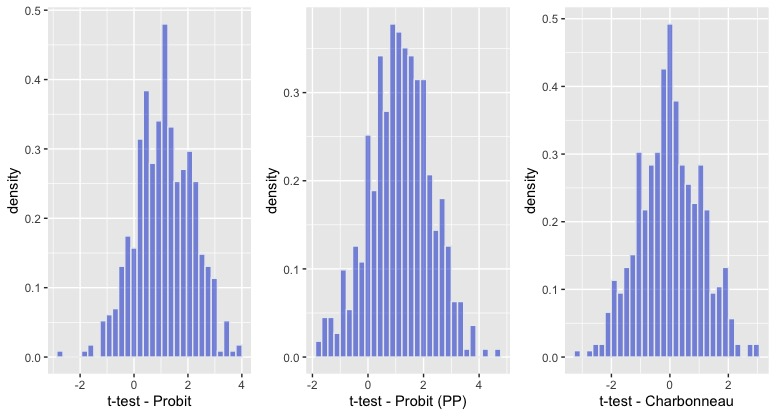
\includegraphics[scale=.4]{content/Figures/ttest_beta22_Design5.png}}
    \caption{\footnotesize{Histogram of the \textit{t-test} for estimated $\beta_{22}^*$ in Design 5}}
    \label{ttest_beta22_Design5}
    \end{adjustwidth}
\end{figure}
\begin{figure}[htbp]
    \vspace{-2.5em}%
    \begin{adjustwidth}{-.5in}{-.5in}
    \centerline{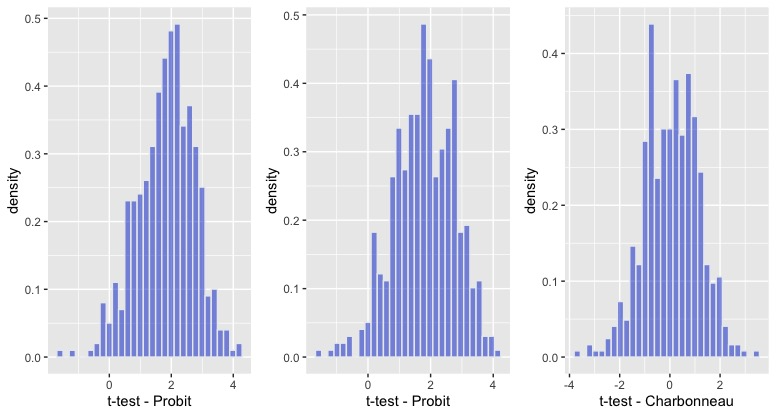
\includegraphics[scale=.4]{content/Figures/ttest_beta23_Design5.png}}
    \caption{\footnotesize{Histogram of the \textit{t-test} for estimated $\beta_{23}^*$ in Design 5}}
    \label{ttest_beta23_Design5}
\end{adjustwidth}
\end{figure}
\begin{figure}[htbp]
    \vspace{-2.5em}%
    \begin{adjustwidth}{-.5in}{-.5in}
    \centerline{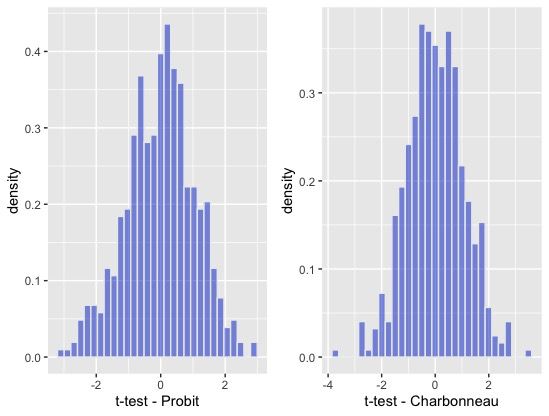
\includegraphics[scale=.4]{content/Figures/ttest_beta22_Design6.png}}
    \caption{\footnotesize{Histogram of the \textit{t-test} for estimated $\beta_{22}^*$ in Design 6}}
    \label{fittest_beta22_Design6g}
\end{adjustwidth}
\end{figure}
\begin{figure}[htbp]
    \vspace{-2.5em}%
    \begin{adjustwidth}{-.5in}{-.5in}
    \centerline{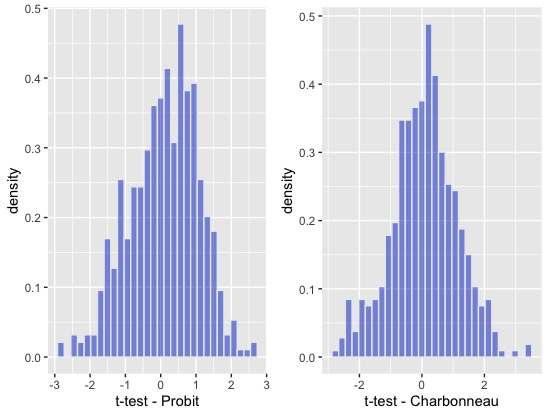
\includegraphics[scale=.4]{content/Figures/ttest_beta23_Design6.png}}
    \caption{\footnotesize{Histogram of the \textit{t-test} for estimated $\beta_{23}^*$ in Design 6}}
    \label{ttest_beta23_Design6}
\end{adjustwidth}
\end{figure}
\begin{figure}[htbp]
    \vspace{-2.5em}%
    \begin{adjustwidth}{-.5in}{-.5in}
    \centerline{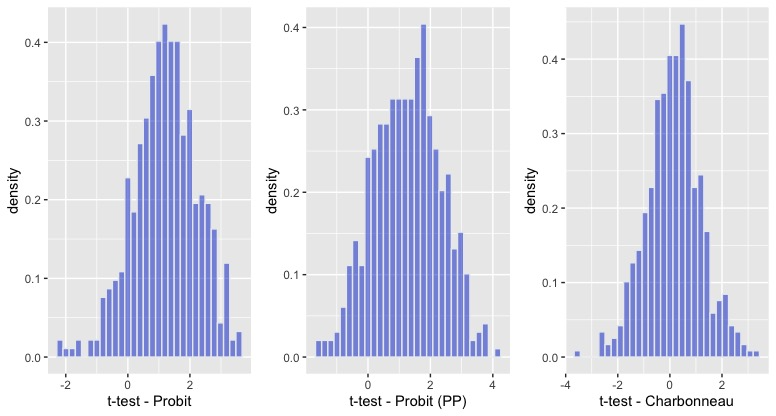
\includegraphics[scale=.4]{content/Figures/ttest_beta22_Design7.png}}
    \caption{\footnotesize{Histogram of the \textit{t-test} for estimated $\beta_{22}^*$ in Design 7}}
    \label{ttest_beta22_Design7}
\end{adjustwidth}
\end{figure}
\begin{figure}[htbp]
    \vspace{-2.5em}%
    \begin{adjustwidth}{-.5in}{-.5in}
    \centerline{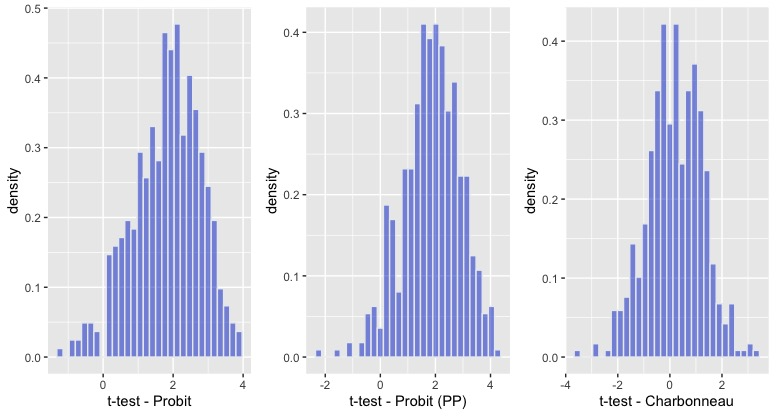
\includegraphics[scale=.4]{content/Figures/ttest_beta23_Design7.png}}
    \caption{\footnotesize{Histogram of the \textit{t-test} for estimated $\beta_{23}^*$ in Design 7}}
    \label{ttest_beta23_Design7}
\end{adjustwidth}
\end{figure}
\begin{figure}[htbp]
    \vspace{-2.5em}%
    \begin{adjustwidth}{-.5in}{-.5in}
\centerline{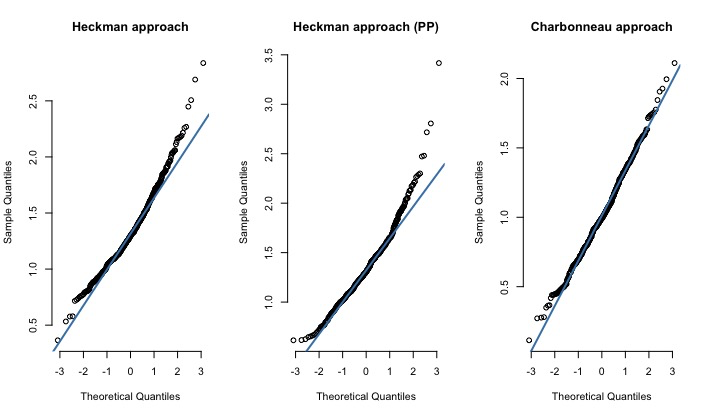
\includegraphics[scale=.4]{content/Figures/QQ_beta_22_Design5.png}}
\caption{\footnotesize{QQ plot of estimated $\beta_{22}^*$ in Design 5}}
\label{QQ_beta_22_Design5}
\end{adjustwidth}
\end{figure}
\begin{figure}[htbp]
    \vspace{-2.5em}%
    \begin{adjustwidth}{-.5in}{-.5in}
\centerline{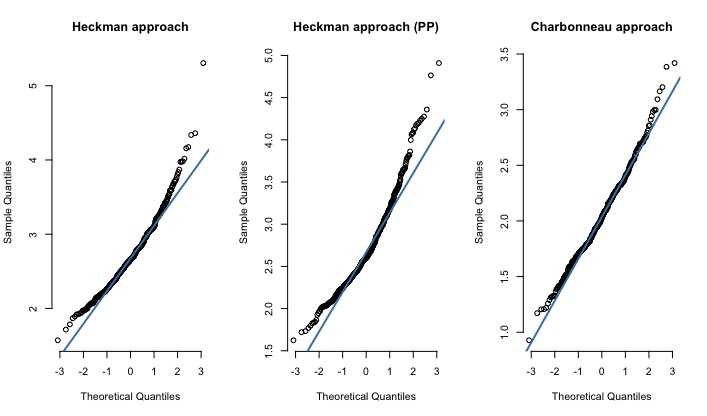
\includegraphics[scale=.4]{content/Figures/QQ_beta_23_Design5.png}}
\caption{\footnotesize{QQ plot of estimated $\beta_{23}^*$ in Design 5}}
\label{QQ_beta_23_Design5}
\end{adjustwidth}
\end{figure}
\begin{figure}[htbp]
    \vspace{-2.5em}%
    \begin{adjustwidth}{-.5in}{-.5in}
\centerline{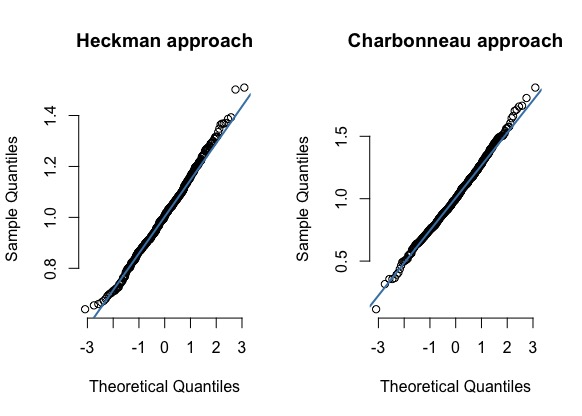
\includegraphics[scale=.4]{content/Figures/QQ_beta_22_Design6.png}}
\caption{\footnotesize{QQ plot of estimated $\beta_{22}^*$ in Design 6}}
\label{QQ_beta_22_Design6}
\end{adjustwidth}
\end{figure}
\begin{figure}[htbp]
    \vspace{-2.5em}%
    \begin{adjustwidth}{-.5in}{-.5in}
\centerline{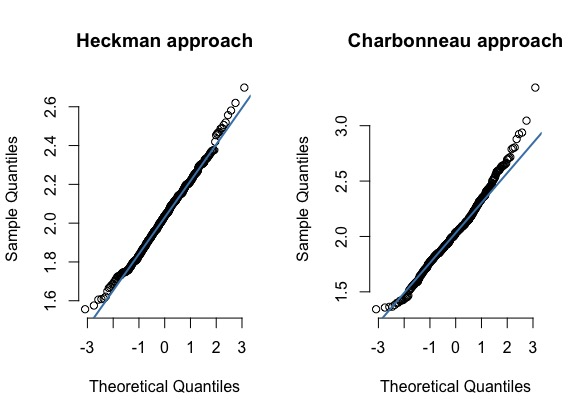
\includegraphics[scale=.4]{content/Figures/QQ_beta_23_Design6.png}}
\caption{\footnotesize{QQ plot of estimated $\beta_{23}^*$ in Design 6}}
\label{QQ_beta_23_Design6}
\end{adjustwidth}
\end{figure}
\begin{figure}[htbp]
    \vspace{-2.5em}%
    \begin{adjustwidth}{-.5in}{-.5in}
    \centerline{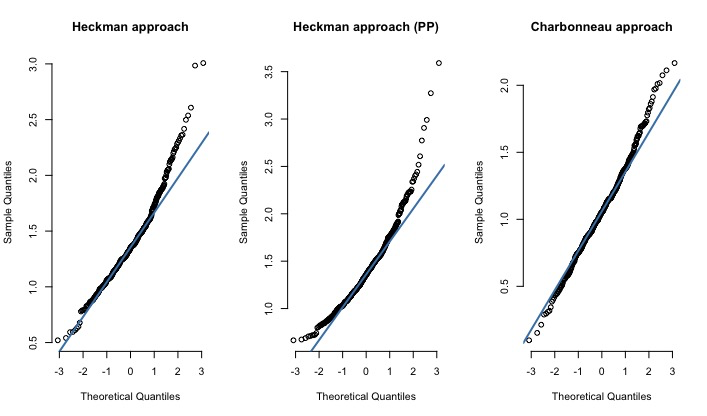
\includegraphics[scale=.4]{content/Figures/QQ_beta_22_Design7.png}}
    \caption{\footnotesize{QQ plot of estimated $\beta_{22}^*$ in Design 7}}
    \label{QQ_beta_22_Design7}
\end{adjustwidth}
\end{figure}
\begin{figure}[htbp]
    \vspace{-2.5em}%
    \begin{adjustwidth}{-.5in}{-.5in}
    \centerline{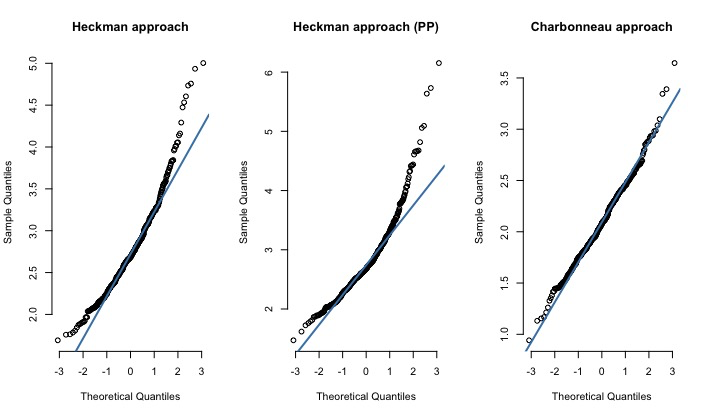
\includegraphics[scale=.4]{content/Figures/QQ_beta_23_Design7.png}}
    \caption{\footnotesize{QQ plot of estimated $\beta_{23}^*$ in Design 7}}
    \label{QQ_beta_23_Design7}
\end{adjustwidth}
\end{figure}
\clearpage
\subsection{Second stage estimates}
\begin{table}
    \begin{adjustwidth}{-.5in}{-.5in}
    \small
    \centering
    \begin{tabular}{p{3cm}p{1.3cm}p{1.3cm}p{1.3cm}p{1.3cm}p{1.3cm}p{1.3cm}p{1.3cm}}
      \hline
       \quad & Design 1 & Design 2 & Design 3 & Design 4 & Design 5 & Design 6 & Design 7  \\
       \hline
       \multicolumn{8}{l}{Hybrid} \\
       \hline
        $\beta_{11}$  & -0.0052 (0.0569) & 0.0000 (0.0747) & 0.0001 (0.0672) & 0.0014 (0.0750) & 0.0014 (0.0893) & 0.0033 (0.0745) & 0.0001 (0.0963) \\
        $\beta_{12}$  & 0.0022 (0.0821) & 0.0042 (0.1336) & 0.0041 (0.1263) & -0.0188 (0.1426) & -0.0026 (0.1547) & 0.0036 (0.1313) & -0.0194 (0.1680)\\
        Inverse Mills-Ratio  &  0.0013 (0.1306) & 0.0036 (0.2508) & 0.0143 (0.2524) & -0.0112 (0.2738)  & 0.0155 (0.3001) & 0.0212 (0.2627) & -0.0030
    (0.2977)\\
         & & & & & & & \\
        \hline
        \multicolumn{8}{l}{Kyriazidou $h=0.5$} \\
       \hline
        $\beta_{11}$  & -0.0054 (0.0759) & 0.0011 (0.0831) & -0.0060 (0.0779) & -0.0046 (0.0837) & 0.0019 (0.0935) & -0.0018 (0.0837) & -0.0067 (0.0887)\\
        $\beta_{12}$  & -0.0010 (0.1305) & -0.0032 (0.1401) & -0.0022 (0.1304) & -0.0082 (0.1431) & 0.0075 (0.1587) &  0.0056 (0.1391) & -0.0032 (0.1551) \\
         & & & & & & & \\
        \hline
        \multicolumn{8}{l}{Kyriazidou $h=0.5$, corrected} \\
       \hline
        $\beta_{11}$  & -0.0054 (0.0762) & 0.0011 (0.0834) & -0.0060 (0.0782) &  -0.0046 (0.0840) & 0.0019 (0.0939) & -0.0018 (0.0840) & -0.0068 (0.0890) \\
        $\beta_{12}$  & -0.0010 (0.1310) & -0.0033 (0.1407)  & -0.0023 (0.1309) & -0.0082 (0.1437) & 0.0074 (0.1593) & 0.0056 (0.1396) & -0.0031 (0.1558) \\
         & & & & & & & \\
        \hline
        \multicolumn{8}{l}{Kyriazidou $h=1$} \\
       \hline
        $\beta_{11}$  & -0.0061 (0.0685) & 0.0011 (0.0746) & -0.0057 (0.0697) & -0.0042 (0.0757) & 0.0000 (0.0841) &  -0.0029 (0.0743) & -0.0062 (0.0788) \\
        $\beta_{12}$  & 0.0001 (0.1161) & -0.0017 (0.1228) & -0.0013 (0.1162) & -0.0124 (0.1254) & 0.0090 (0.1403) &  0.0071 (0.1270) & -0.0083 (0.1361) \\
         & & & & & & & \\
            \hline
        \multicolumn{8}{l}{Kyriazidou $h=1$, corrected} \\
       \hline
        $\beta_{11}$  & -0.0062 (0.0687) & 0.0010 (0.0748) & -0.0058 (0.0699) & -0.0043 (0.0759) & 0.0000 (0.0843) &  -0.0030 (0.0745) & -0.0064 (0.0791) \\
        $\beta_{12}$  & 0.0001 (0.1164) & -0.0018 (0.1231) & -0.0015 (0.1165) & -0.0125 (0.1257) & 0.0090 (0.1407) &  0.0070 (0.1273) & -0.0083 (0.1364)\\
         & & & & & & & \\
        \hline
        \multicolumn{8}{l}{Kyriazidou $h=2$} \\
        \hline
         $\beta_{11}$  & -0.0063 (0.0647) & 0.0010 (0.0699) & -0.0048 (0.0641) & -0.0029 (0.0699) &-0.0012 (0.0785)  & -0.0036 (0.0686) & -0.0050 (0.0726)\\
         $\beta_{12}$  & 0.0000 (0.1098) & 0.0001 (0.1150) & 0.0000 (0.1097) & -0.0145 (0.1172) & 0.0084 (0.1324) & 0.0064 (0.1207) & -0.0103 (0.1256) \\
         & & & & & & & \\
         \hline
         \multicolumn{8}{l}{Kyriazidou $h=2$, corrected} \\
        \hline
         $\beta_{11}$  & -0.0066 (0.0649) & 0.0001 (0.0700) & -0.0052 (0.0643) & -0.0033 (0.0701) & -0.0014 (0.0787) &  -0.0040 (0.0688) & -0.0052 (0.0728) \\
         $\beta_{12}$  & 0.0000 (0.1100) & 0.0000 (0.1152) & -0.0001 (0.1099) & -0.0149 (0.1174) & 0.0082 (0.1327) &  0.0060 (0.1209) & -0.0106 (0.1258)\\
              & & & & & & & \\
         \hline
    \end{tabular}
    \caption{\footnotesize{Simulation results for the estimated coefficients for the observation Equation \ref{eq:dgp1} with $N=25$ and 500 iterations. For these results, we set the values of the parameters from the first stage Equation \ref{eq:dgp3} to be equal to their true values. The values correspond to the mean bias of estimates, and the standard deviation is in parenthesis.}}
    \label{tab:4}
    \end{adjustwidth}
\end{table}

\begin{table}
    \begin{adjustwidth}{-.5in}{-.5in}
    \small
    \centering
    \begin{tabular}{p{3cm}p{1.3cm}p{1.3cm}p{1.3cm}p{1.3cm}p{1.3cm}p{1.3cm}p{1.3cm}}
      \hline
       \quad & Design 1 & Design 2 & Design 3 & Design 4 & Design 5 & Design 6 & Design 7  \\
       \hline
        \multicolumn{8}{l}{Kyriazidou $h=3$} \\
       \hline
        $\beta_{11}$  & -0.0060 (0.0632) & 0.0011 (0.0685) & -0.0039 (0.0622) & -0.0019 (0.0675) & -0.0001 (0.0763) &  -0.0033 (0.0665) & -0.0038 (0.0700) \\
        $\beta_{12}$  & 0.0000 (0.1081) & 0.0019 (0.1128) & 0.0000 (0.1078) & -0.0139 (0.1146) & 0.0085 (0.1290) & 0.0065 (0.1176) & -0.0097 (0.1224) \\
        & & & & & & & \\
        \hline
        \multicolumn{8}{l}{Kyriazidou $h=3$, corrected} \\
       \hline
        $\beta_{11}$  & -0.0065 (0.0634) & 0.0001 (0.0686) & -0.0045 (0.0623) & -0.0024 (0.0677) & -0.0013 (0.0766) & -0.0038 (0.0667) & -0.0042 (0.0702)\\
        $\beta_{12}$  & 0.0000 (0.1083) & 0.0013 (0.1130) & 0.0000 (0.1080) & -0.0145 (0.1148) & 0.0081 (0.1293) &  0.0059 (0.1178) & -0.0101 (0.1226)\\
                 & & & & & & & \\
        \hline
        \multicolumn{8}{l}{Kyriazidou $h=5$} \\
       \hline
        $\beta_{11}$  & -0.0042 (0.0615) & 0.0020 (0.0672) & -0.0020 (0.0606) & 0.0001 (0.0649) & 0.0001 (0.0740) &  -0.0011 (0.0645) & -0.0015 (0.0673)\\
        $\beta_{12}$  & 0.0029 (0.1062) & 0.0040 (0.1103) & 0.0021 (0.1058) & -0.0117 (0.1123) & 0.0100 (0.1254) &  0.0082 (0.1141) & -0.0080 (0.1198) \\
        & & & & & & & \\
        \hline
        \multicolumn{8}{l}{Kyriazidou $h=5$, corrected} \\
       \hline
        $\beta_{11}$  & -0.0050 (0.0617) & 0.0014 (0.0674) & -0.0028 (0.0608) & 0.0000 (0.0651) & 0.0000 (0.0742) &  -0.0018 (0.0647) & -0.0020 (0.0675)\\
        $\beta_{12}$  & 0.0020 (0.1065) & 0.0032 (0.1106) & 0.0012 (0.1060) & -0.0125 (0.1125) & 0.0094 (0.1257) &  0.0073 (0.1143) & -0.0086 (0.1201) \\
                     & & & & & & & \\
        \hline
        \multicolumn{8}{l}{Kyriazidou $h=10$} \\
       \hline
        $\beta_{11}$  & 0.0046 (0.0583) & 0.0090 (0.0646) & 0.0070 (0.0578) & 0.0091 (0.0613) & 0.0067 (0.0702) &  0.0073 (0.0612) & 0.0050 (0.0637) \\
        $\beta_{12}$  & 0.0147 (0.1023) & 0.0128 (0.1074) & 0.0123 (0.1029) & -0.0026 (0.1090) & 0.0168 (0.1206) & 0.0180 (0.1096) & -0.0016 (0.1160)\\
        & & & & & & & \\
        \hline
        \multicolumn{8}{l}{Kyriazidou $h=10$, corrected} \\
       \hline
        $\beta_{11}$  & 0.0037 (0.0584) & 0.0083 (0.0648) & 0.0061 (0.0580) & 0.0083 (0.0615) & 0.0062 (0.0704) &  0.0065 (0.0614) & 0.0045 (0.0639)\\
        $\beta_{12}$  & 0.0136 (0.1025) & 0.0120 (0.1076) & 0.0112 (0.1031) & -0.0035 (0.1092) & 0.0162 (0.1208) & 0.0170 (0.1098) & -0.0022 (0.1162) \\
        \hline
    \end{tabular}
    \caption{\footnotesize{Simulation results for the estimated coefficients for the observation Equation \ref{eq:dgp1} with $N=25$ and 500 iterations. For these results, we set the values of the parameters from the first stage Equation \ref{eq:dgp3} to be equal to their true values. The values correspond to the mean bias of estimates, and the standard deviation is in parenthesis.}}
    \label{tab:5}
    \end{adjustwidth}
\end{table}
\begin{figure}[htbp]
    \begin{adjustwidth}{-.5in}{-.5in}
        \centerline{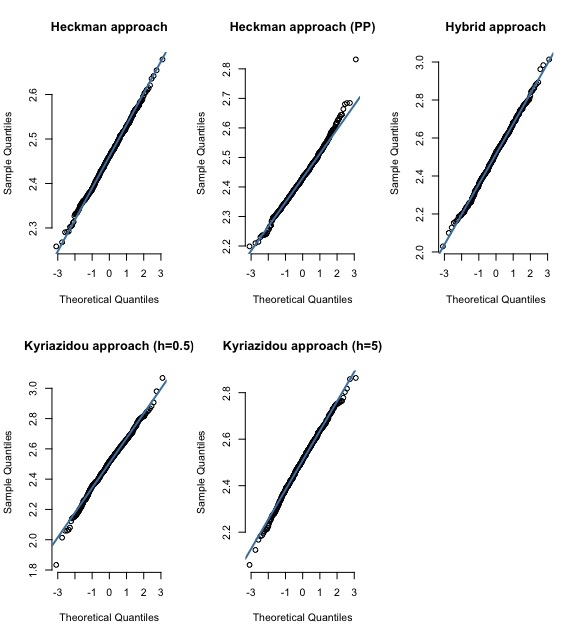
\includegraphics[scale=.4]{content/Figures/QQ_beta_12_Design5.png}}
        \caption{\footnotesize{QQ plot of estimated $\beta_{12}$ in Design 5}}
        \label{QQ_beta_12_Design5}
    \end{adjustwidth}
\end{figure}    
\begin{figure}[htbp]
    \vspace{-2.5em}%
    \begin{adjustwidth}{-.5in}{-.5in}
        \centerline{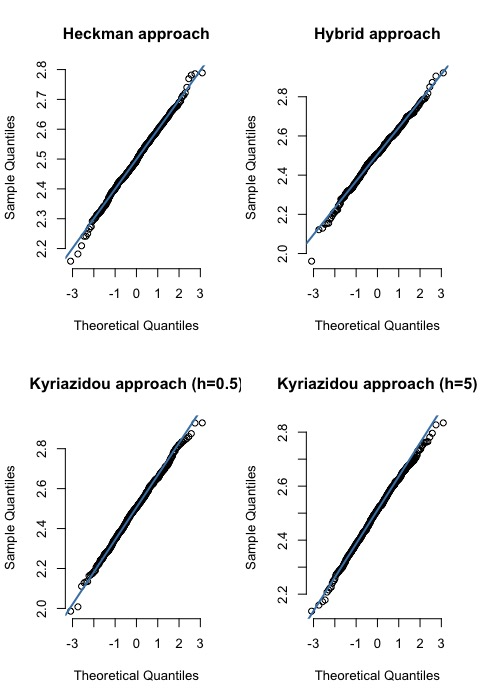
\includegraphics[scale=.4]{content/Figures/QQ_beta_12_Design6.png}}
        \caption{\footnotesize{QQ plot of estimated $\beta_{12}$ in Design 6}}
        \label{QQ_beta_12_Design6}
    \end{adjustwidth}
\end{figure}     
\begin{figure}[htbp]
    \vspace{-2.5em}%
    \begin{adjustwidth}{-.5in}{-.5in}
        \centerline{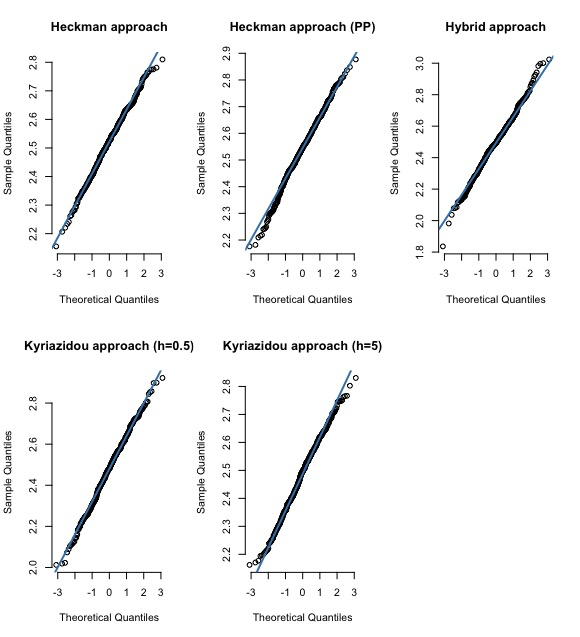
\includegraphics[scale=.4]{content/Figures/QQ_beta_12_Design7.png}}
        \caption{\footnotesize{QQ plot of estimated $\beta_{12}$ in Design 7}}
        \label{QQ_beta_12_Design7}
    \end{adjustwidth}
\end{figure}



\end{document}
